\chapter{UAV (Unmanned Aerial Vehicle)}
\section{Quad-copter (Drone)}
\subsection{Introduction} 
\par  Innovative work on unmanned aerial vehicles (UAVs) is getting high consolation these days, since the applications of UAV can apply to many areas such as military, salvage mission, film making, farming, and others.
In remote areas like border areas or agricultural fields to monitor the situations on a daily basis, for surveillance in those areas, Unmanned Aerial Vehicle(UAV) plays an important role. UAV is also known as Drone and has a lot of attention nowadays. Drones are generally used at the border areas which cannot be done manually by military forces.
The quad-copter works according to the force or thrust generated by four rotors connected to its body. It has four input and six yield or output states ($x$, $y$, $z$, $\theta$, $\psi$, $\omega$), and it is an under-activated framework, since this empowers quad-copter has to convey more load.
\subsection{Quad-copter Motion Mechanism}
\par Quad-copter can be described as a vehicle with four propellers joined to the rotor found at the cross casing. This goes for altered pitch rotors driven to control the vehicle movement. The velocities of these four rotors are independent. By controlling the pitch, roll and yaw angle, the position of the vehicle can be controlled effectively.
\par Quad-copter has four inputs, and essentially the thrust is generated by the propellers attached to the rotors. The speed of each motor is controlled independently, and the motion or direction of the quad-copter is controlled by varying the speed and direction of each motor.
\begin{figure}[h!]
\centering
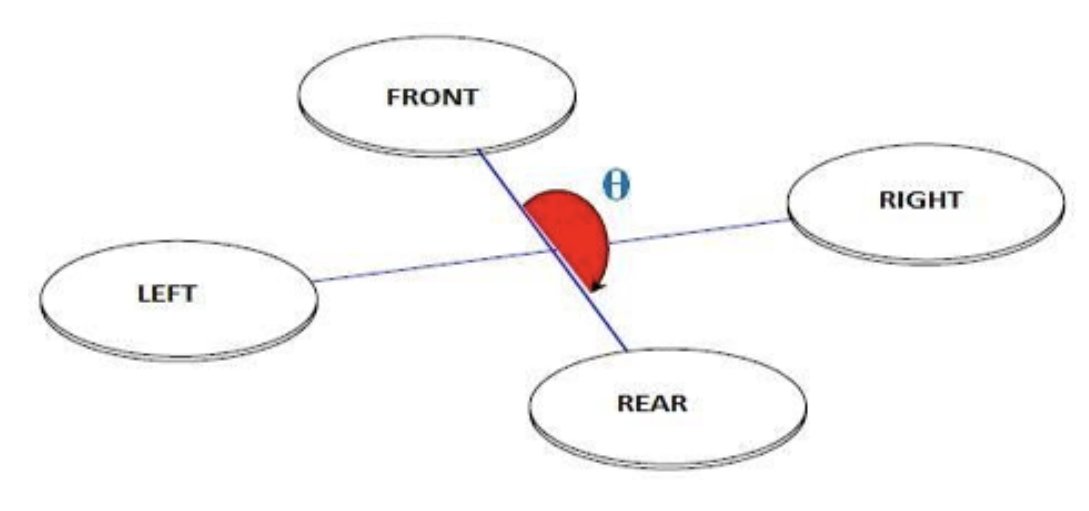
\includegraphics[width=10cm]{./Figures/pitch_direction.png}
\caption{Pitch direction of quad-copter}
\label{Pitch_direction_of_quadcopter}
\end{figure}

\begin{figure}[h!]
\centering
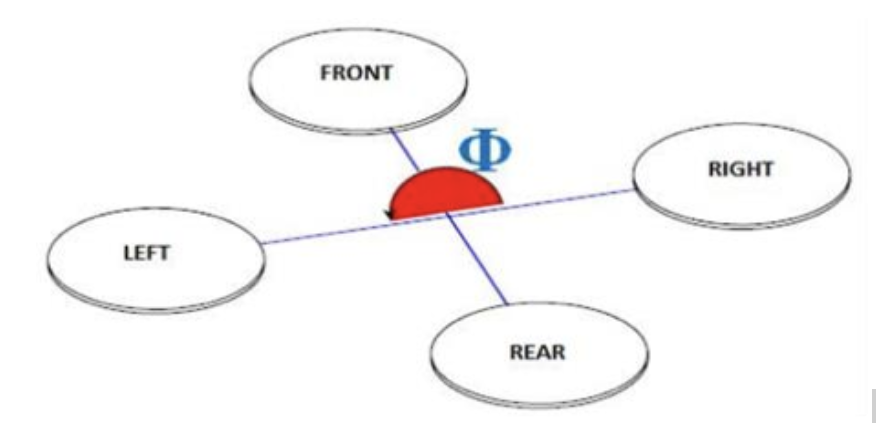
\includegraphics[width=10cm]{./Figures/roll_direction.png}
\caption{Roll direction of quad-copter}
\label{Roll_direction_of_quadcopter}
\end{figure}

\begin{figure}[h!]
\centering
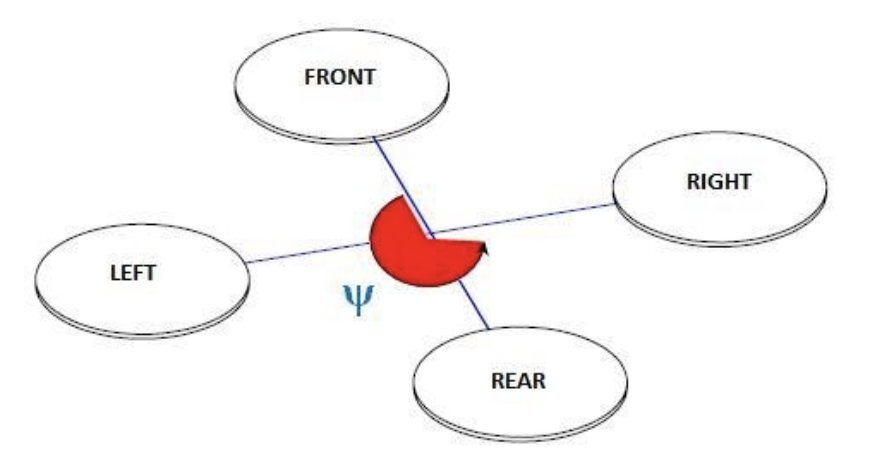
\includegraphics[width=10cm]{./Figures/yaw_dir_qc.png}
\caption{Yaw direction of quad-copter}
\label{Yaw_direction_of_quadcopter}
\end{figure}

\subsection{Take-off and Landing Motion Mechanism}
\par Take-off motion is the motion that lifts the quad-copter from ground to hover position. As shown in Fig.2.4 there are a total four motors, two rotating in the clockwise direction and two rotating in counter clockwise direction. To fly the quad-copter in hover position, increase the speed of each rotor simultaneously. For landing the quad-copter to ground decrease the speed of each rotor simultaneously as shown in Fig.2.5.

\begin{figure}[h!]
\centering
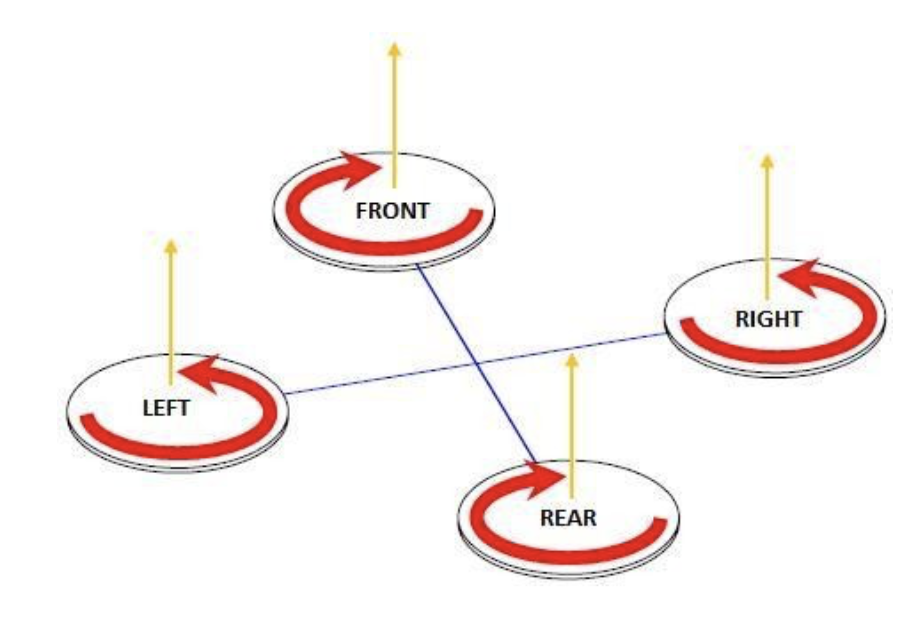
\includegraphics[width=10cm]{./Figures/takeoff_qc.png}
\caption{Take-off motion}
\label{Take_off_motion}
\end{figure}

\begin{figure}[h!]
\centering
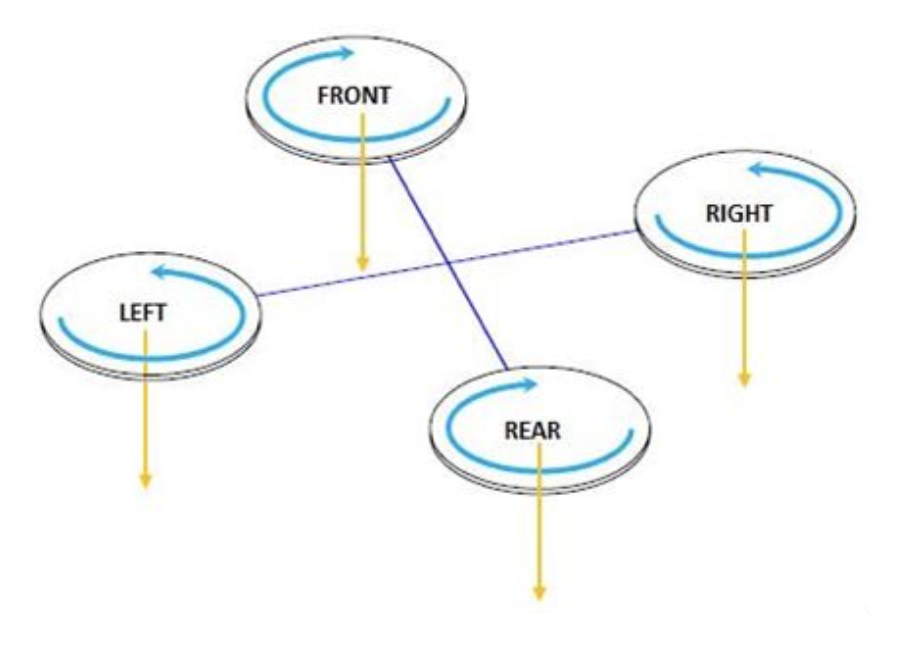
\includegraphics[width=10cm]{./Figures/landing_motion_qc.png}
\caption{Landing Motion}
\label{Landing_Motion}
\end{figure}

\subsection{Forward and Backward Motion Mechanism}
\par Forward motion of the quad-copter is controlled by increasing the speed of the rear rotor and decreasing the speed of the front rotor simultaneously as shown in Fig.2.6. Backward motion of the quad-copter is controlled by increasing the speed of the front rotor and decreasing the speed of the rear rotor simultaneously as shown in Fig.2.7. Reducing the rear rotor speed and increasing the front rotor speed simultaneously will affect the pitch angle of the quad-copter.

\begin{figure}[h!]
\centering
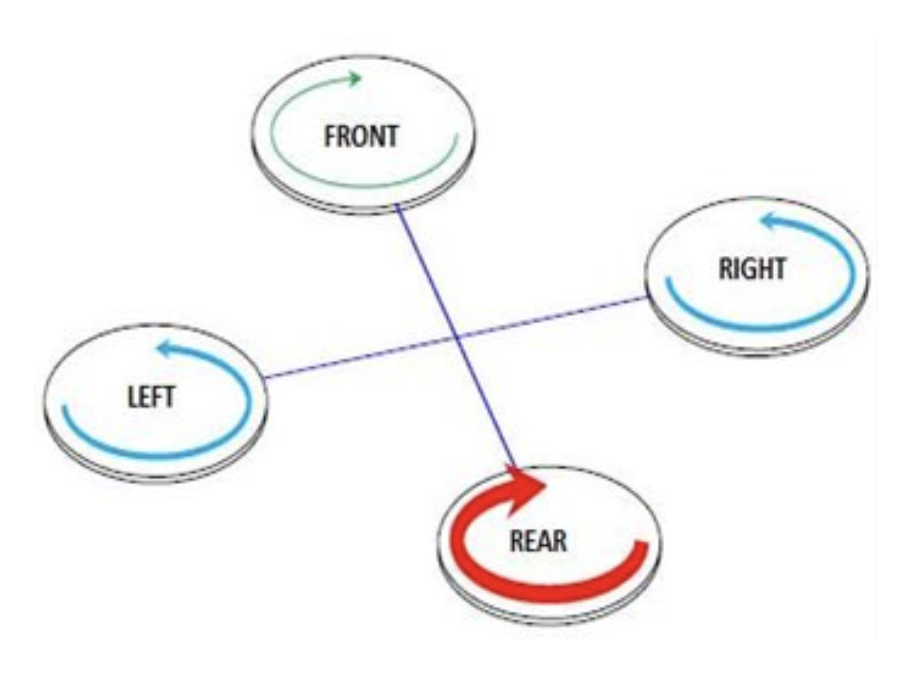
\includegraphics[width=10cm]{./Figures/forward_motion_qc.png}
\caption{Forward motion}
\label{Forward_motion}
\end{figure}

\begin{figure}[h!]
\centering
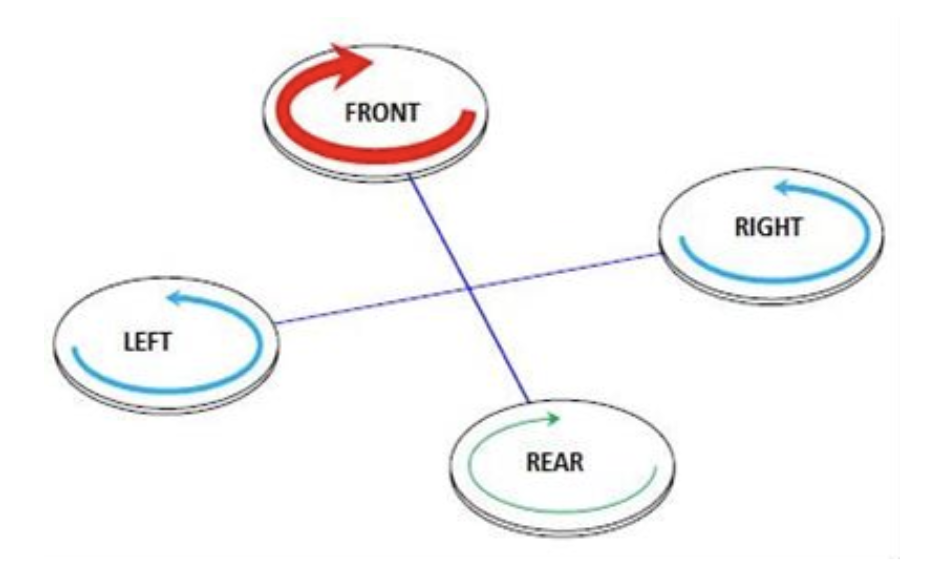
\includegraphics[width=10cm]{./Figures/backward_motion_qc.png}
\caption{Backward motion}
\label{Backward_motion}
\end{figure}

\subsection{Left and Right Motion Mechanism}
\par The left and right motions of the quad-copter are controlled by changing the yaw angle. By increasing the speed of the counter-clockwise rotor and decreasing the speed of the clockwise rotor simultaneously, the quad-copter moves to the left side as shown in Fig.2.8. Similarly by increasing the speed of the clockwise rotor and decreasing the speed of the counter-clockwise rotor simultaneously, the quad-copter moves to the right side as shown in Fig.2.8.

\begin{figure}[h!]
\centering
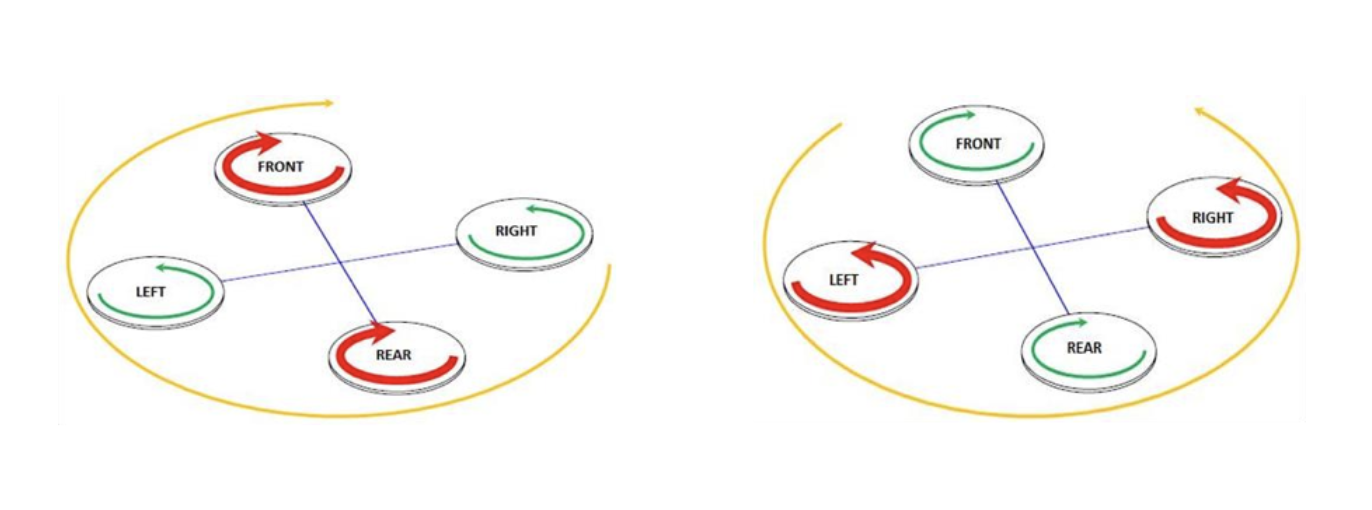
\includegraphics[width=\columnwidth]{./Figures/left_ryt_motion_qc.png}
\caption{Left and right motion}
\label{Left_and_right_motion}
\end{figure}

\subsection{Hovering and Static Position}
\par When two pairs of counter-clockwise and clockwise rotors rotate at the same speed, the quad-copter moves to hover position. At that time, the total addition of reaction torque is zero which allows the quad-copter to achieve hover position.

\newpage
\subsection{Hardware requirements}
\begin{table}[h!]
\centering
\begin{tabular}{|l|l|l|} 
\hline
\textbf{Description}               & \textbf{Make~} & \textbf{Model}       \\ 
\hline
Frame(Quad-copter 4 axis)          & -              & F450                 \\ 
\hline
Motor (1000Kv)                     & -              & A2212/13T            \\ 
\hline
ESC (30 Amp)                       & Simonk         & 30A                  \\ 
\hline
APM Controller (2.8)               & ArduPilot      & APM 2.8              \\ 
\hline
Transmitters and Receiver~         & Flysky~        & Fs-i6 2.4Ghz         \\ 
\hline
Duracell Batteries for Transmitter & Duracell       & Ultra (Alkaline AA)  \\ 
\hline
GPS                                & Ublox~         & NEO 5 pin            \\ 
\hline
Battery~ (2200mAh 3S, ,11V)        & Shang yi       & B3 - 2200 mAH        \\ 
\hline
Battery Chargers (B3)              & imaxRC         & B3 pro~              \\ 
\hline
Propellers~ pairs (CW and ACW)     & -              & (10*4.5inch)         \\
\hline
\end{tabular}
\caption{Hardware components for UAV}
\end{table}

\subsubsection{Frame ( Quad-copter 4 axis F450):}
\begin{figure}[h!]
\centering
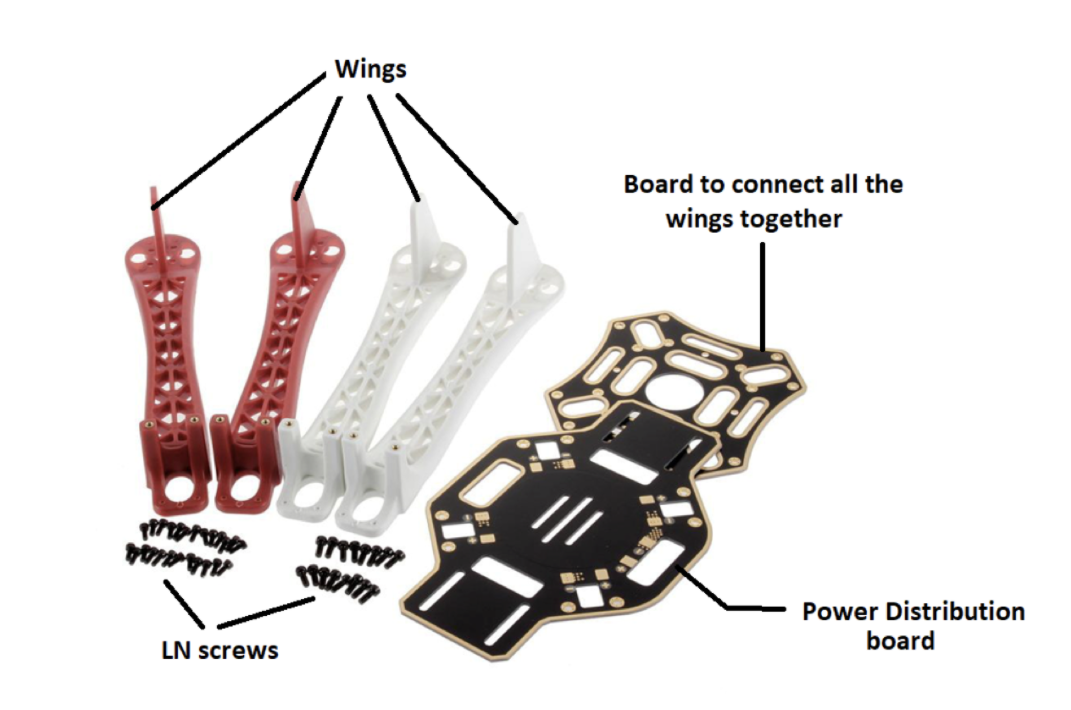
\includegraphics[width=\columnwidth]{./Figures/frame_qc.png}
\caption{Frame ( Quad-copter 4 axis F450)}
\label{frame_qc}
\end{figure}

\newpage
\subsubsection{Direction of Motion w.r.t. Frame:}
\begin{figure}[h!]
\centering
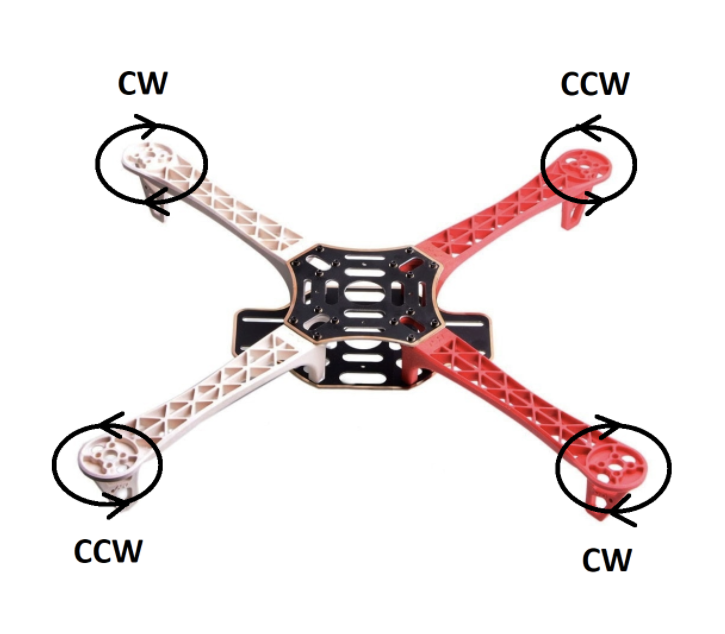
\includegraphics[width=10cm]{./Figures/dir_of_motion_wrt_frame.png}
\caption{Direction of Motion w.r.t. Frame:}
\label{dir_of_motion_wrt_frame}
\end{figure}


\subsubsection{Motors (A2212/13T):}
\begin{figure}[h!]
\centering
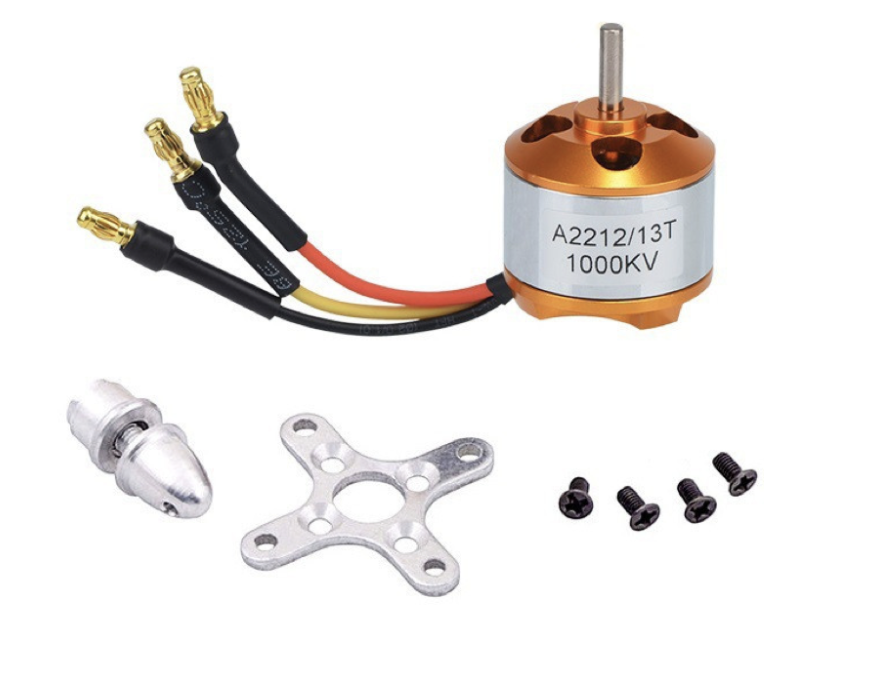
\includegraphics[width=8cm]{./Figures/motors_qc.png}
\caption{Motors (A2212/13T)}
\label{motors_qc}
\end{figure}

\begin{itemize}
    \item KV rating : 1000 kV
    \item Operating voltage : 12V
    \item Idle Current: 0.5 A
    \item Motor Dimensions: 27.5 x 30mm
    \item Shaft diameter : 3.175mm. 
    \item Weight: 47 g
\end{itemize}

\subsubsection{Electronic Speed Controllers (ESCs):}
\begin{figure}[h!]
\centering
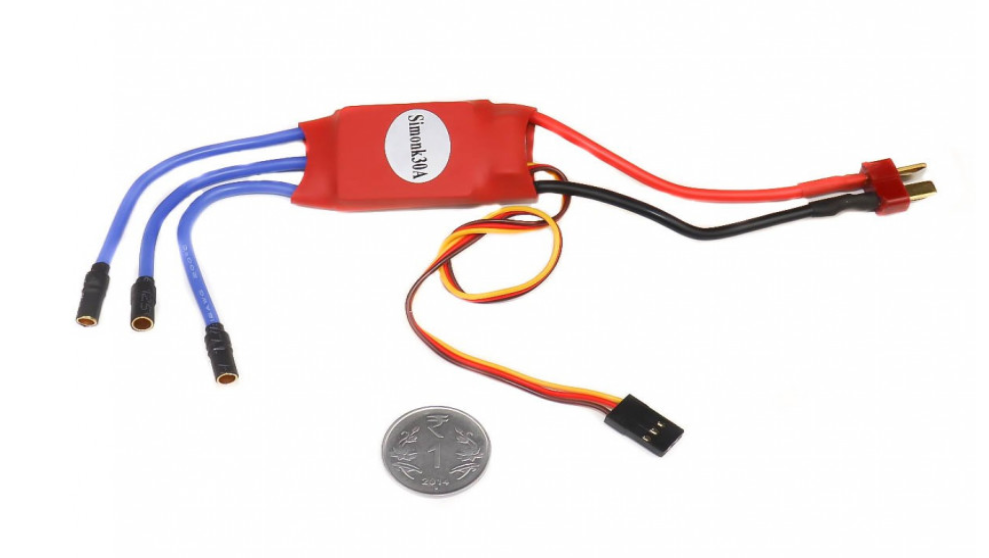
\includegraphics[width=12cm]{./Figures/esc_qc.png}
\caption{Electronic Speed Controllers (ESCs)}
\label{esc_qc}
\end{figure}

\begin{itemize}
    \item Output: 
    \begin{itemize}
        \item 30A continuous 
        \item 40Amps for 10 seconds
    \end{itemize}
    \item Input voltage: 2-4 cells Lithium Polymer
    \item BEC : 5V, 3Amp for external receiver and servos
    \item Max Speed: 
    \begin{itemize}
        \item 2 Pole: 210,000rpm
        \item 6 Pole: 70,000rpm
        \item 12 Pole: 35,000rpm
    \end{itemize}
    \item Weight: 32gms
    \item Size: 55mm x 26mm x 13mm 
\end{itemize}


% \subsubsection{Connection of ESC:}
\begin{figure}[h!]
\centering
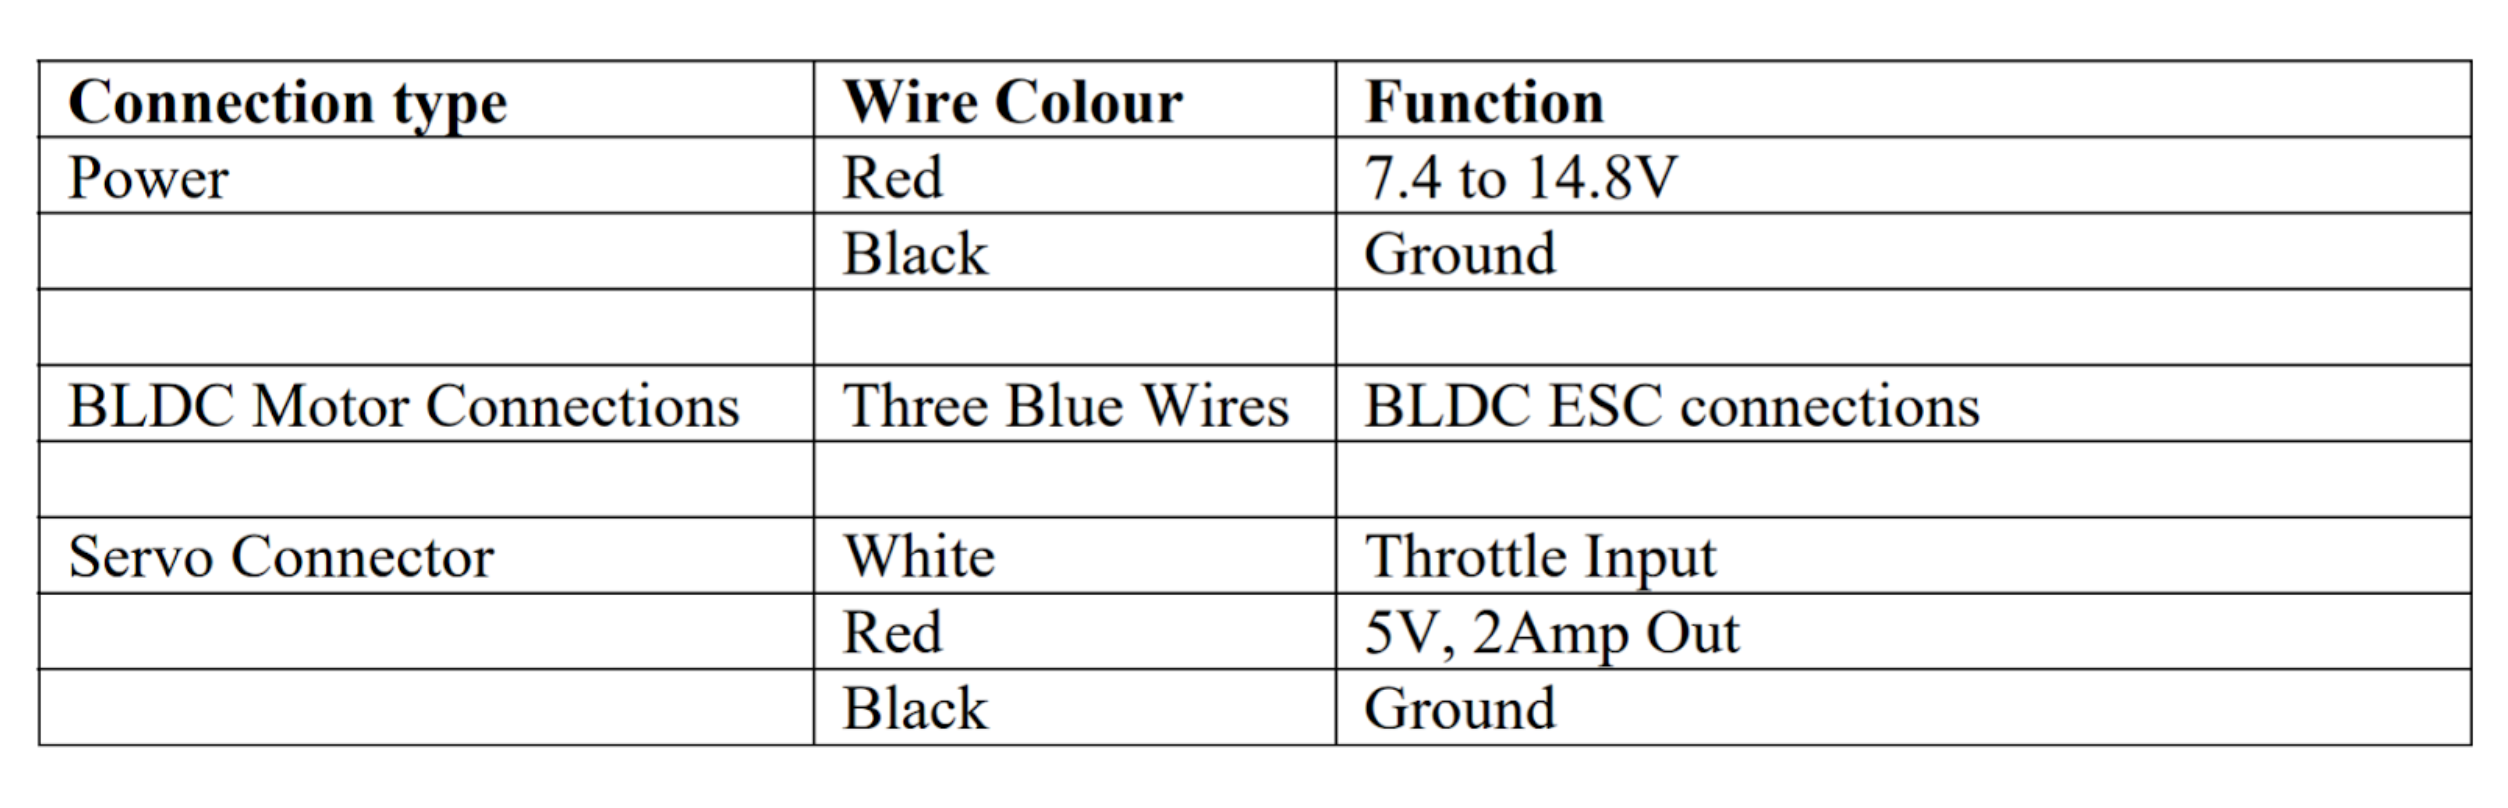
\includegraphics[width=\columnwidth]{./Figures/conn_esc_specs.png}
\caption{Connection between ESC and BLDC motor.}
\label{conn_esc_specs}
\end{figure}

\subsubsection{Transmitter (Fly-sky FS6iAB):}
\begin{figure}[h!]
\centering
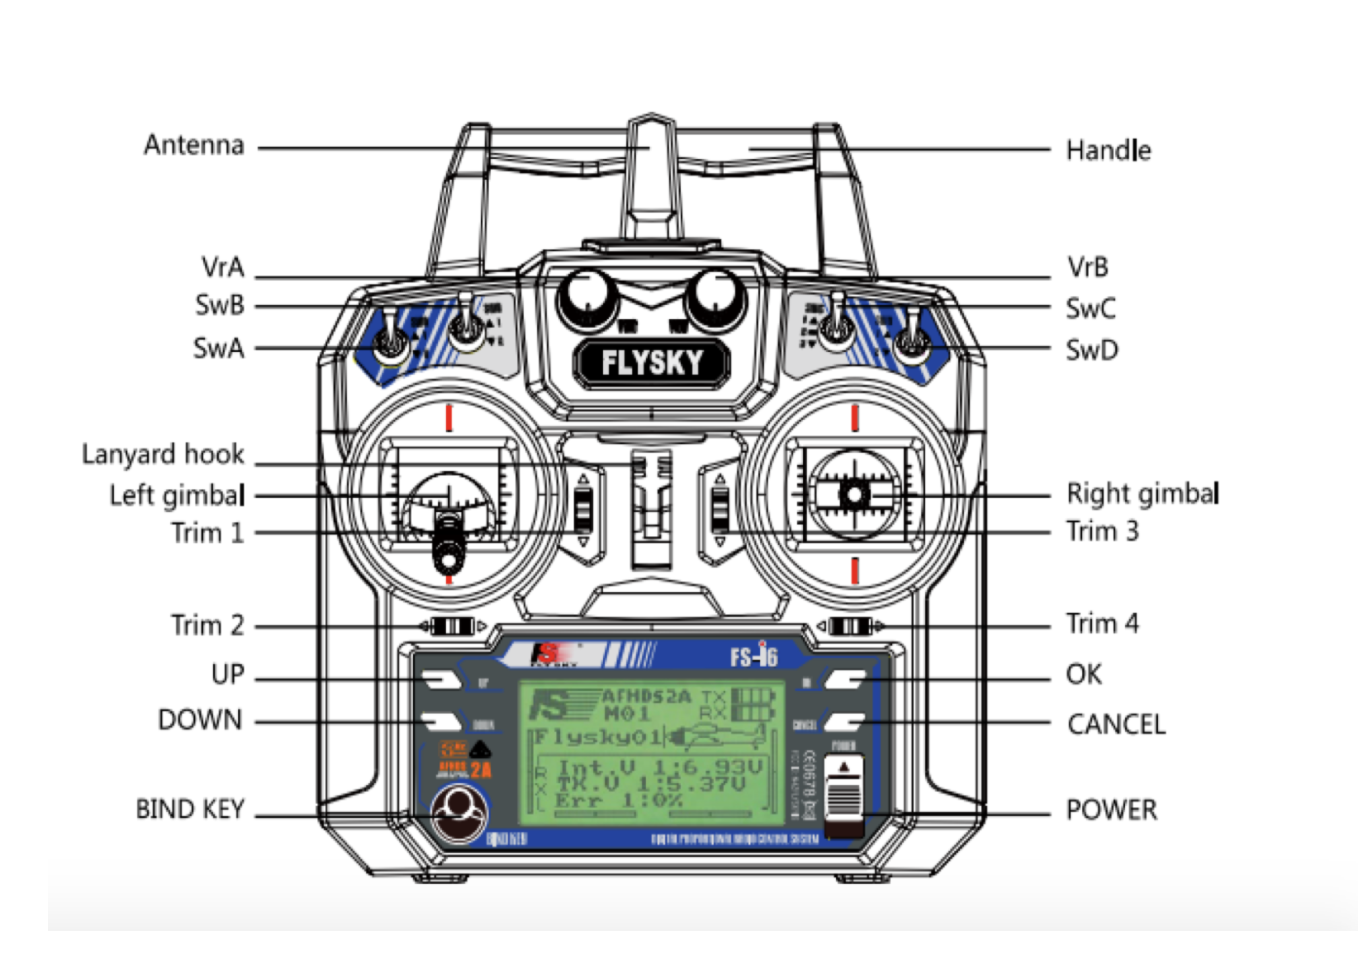
\includegraphics[width=\columnwidth]{./Figures/transmitter_qc.png}
\caption{Transmitter (Fly-sky FS6iAB)}
\label{transmitter_qc}
\end{figure}

\begin{itemize}
    \item Model type 		: Quad-copter
    \item  RF range 		: 2.408 - 2.475GHz
    \item Bandwidth 		: 500 KHz
    \item Bands 		             : 135
    \item RF power 		: Less than 20 dBm
    \item Protocol 		: AFHDS 2A
    \item Modulation type 	: GFSK
    \item PS2/USB Port 		: Yes (Micro-USB)
    \item Power input 		: 6V DC 1.4AA*4
    \item Weight		             : 392g
    \item Size 			: 174 x 89 x 190 mm
    \item Color 			: Black 
\end{itemize}

\subsubsection{Receiver (Fly-sky FS6iAB)}
\begin{figure}[h!]
\centering
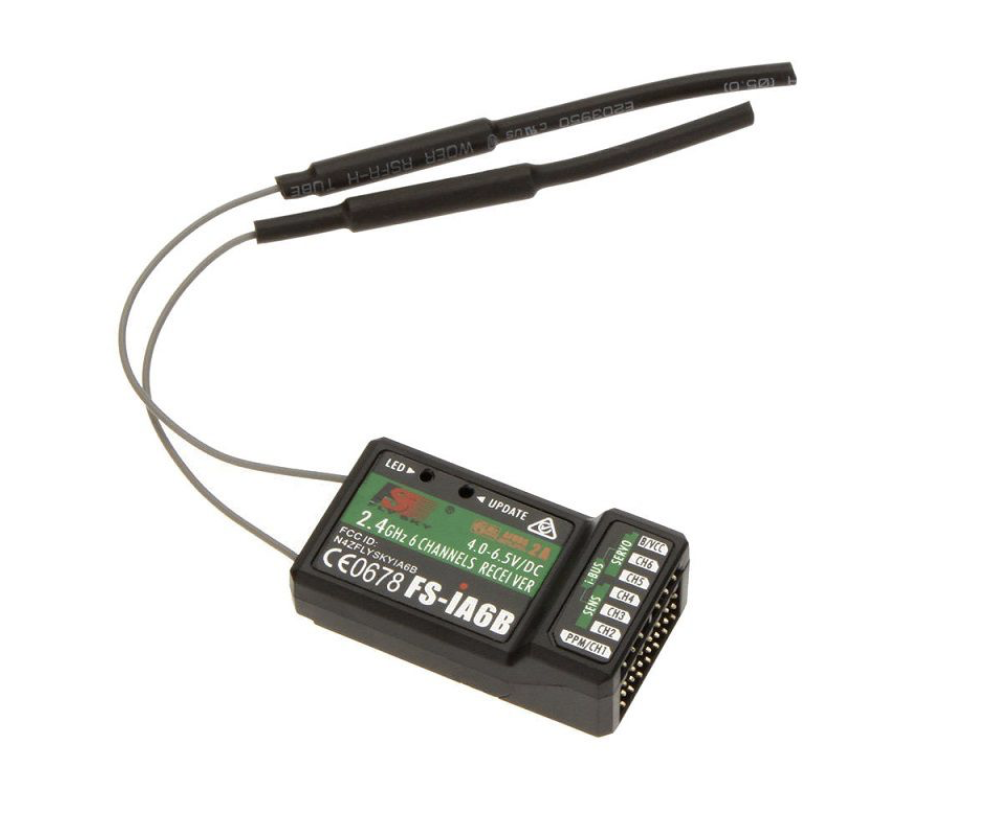
\includegraphics[width=8cm]{./Figures/receiver_qc.png}
\caption{Receiver (Fly-sky FS6iAB)}
\label{receiver_qc}
\end{figure}

\begin{itemize}
    \item Channels 		: 6
    \item RF range 		: 2.408 - 2.475GHz
    \item Bandwidth 		: 500 KHz
    \item Bands	             		: 135
    \item RF power 		: Less than 20 dBm
    \item Rx sensitivity 		: ~105 dBm
    \item Protocol 		: AFHDS 2A
    \item Modulation type 	: GFSK
    \item Power input 		: 4 – 6.5 V DC
    \item Antenna length 		: 26 mm x 2
    \item Weight			: 7g
    \item Size 			: 40 x 21 x 15 mm
   \item Color 			: Black
\end{itemize}

\subsubsection{Controller (Ardupilot APM 2.8):}
\begin{figure}[h!]
\centering
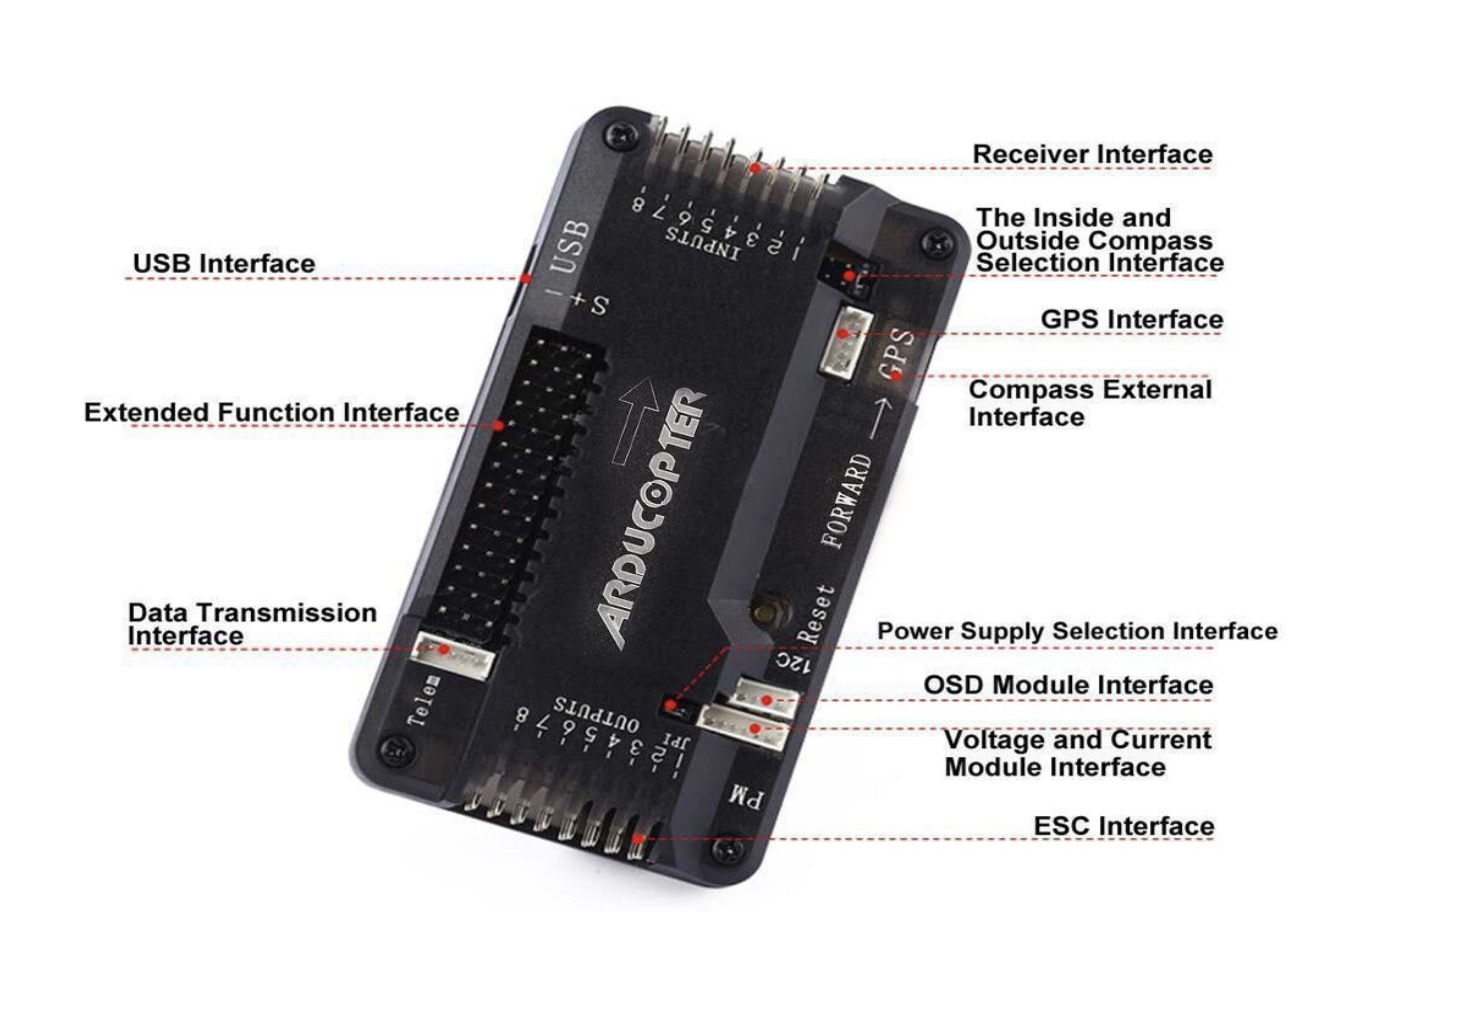
\includegraphics[width=12cm]{./Figures/controller_qc.png}
\caption{Controller (Ardupilot APM 2.8)}
\label{controller_qc}
\end{figure}

\begin{table}[h!]
\centering
\begin{tabular}{|l|l|} 
\hline
Model                 & : APM 2.8                     \\ 
\hline
Power supply          & : LP2985-3.3.                 \\ 
\hline
Input Voltage (V)     & : 12\textasciitilde{}16 VDC   \\ 
\hline
Sensors               & : 3-Axis Gyrometer            \\ 
\hline
~                     & ~ Accelerometer               \\ 
\hline
~                     & ~ High-performance Barometer  \\ 
\hline
Processor             & : ATMEGA2560 and ATMEGA32U-2  \\ 
\hline
Dimensions (mm) LxWxH & : 70 x 45 x 15                \\ 
\hline
Weight (gm)           & : 82                          \\ 
\hline
Shipment Weight       & : 0.085 kg                    \\ 
\hline
Shipment Dimensions   & : 9 × 3 × 2 cm                \\
\hline
\end{tabular}
\end{table}

\newpage

\subsubsection{GPS Module:}
\begin{figure}[h!]
\centering
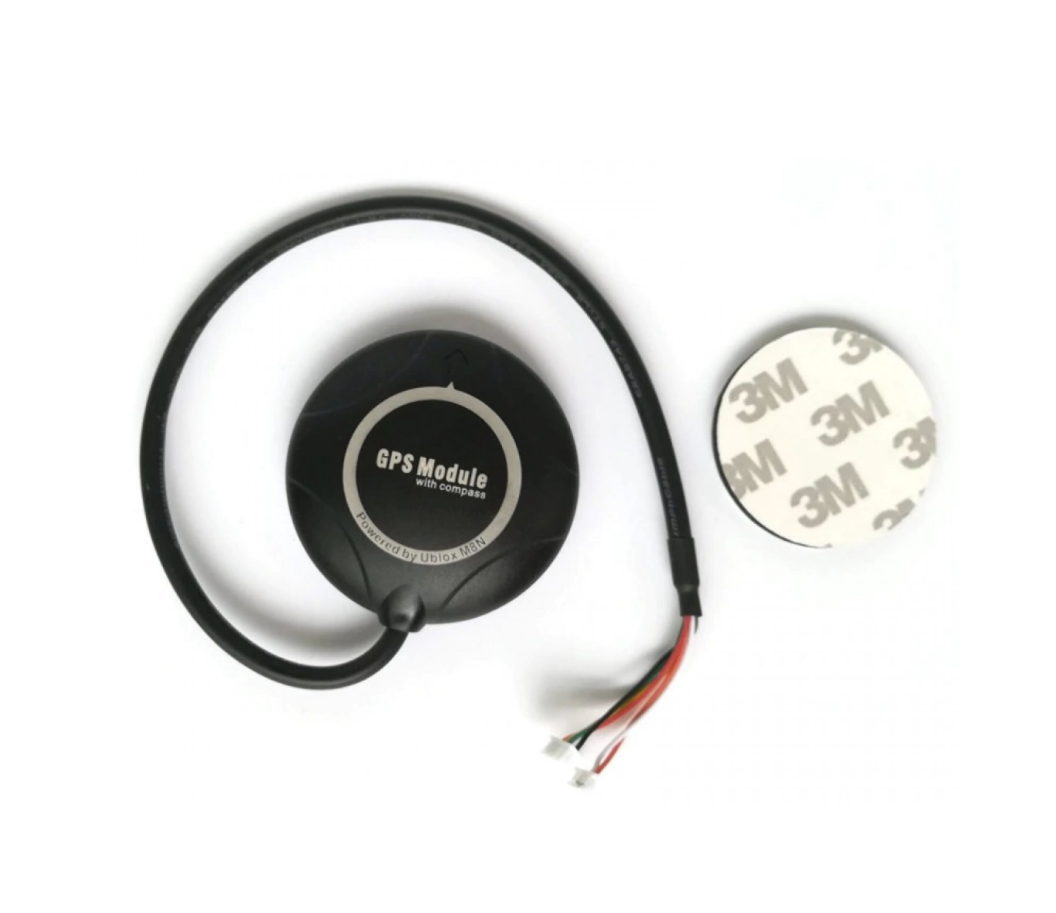
\includegraphics[width=10cm]{./Figures/gps_qc.png}
\caption{GPS Module}
\label{gps_qc}
\end{figure}

\begin{itemize}
    \item Model				: FPV Ublox NEO-M8N
    \item Receiver Type			: 72-channel Ublox M8 engine.
    \item Main Chip			: Ublox NEO-M8N
    \item Sensitivity			: Cold starts: –148 dBm. Hot starts: –156 dBm.
    \item Position Accuracy		: Autonomous: 2.5 m SBAS: 2.0 m
    \item Acceleration			: $<$4g
    \item Navigation Update Rate		: up to 18 HZ.
    \item Operating Temperature Range	: -24ºC ~ 84°C
    \item Tracking Sensitivity		: –167 dBm.
    \item Capture Time			: 0.1s Average
    \item Dimensions (mm)	: 50 x 12.8 (Diameter x W)
    \item Weight (gm)			: 28
    \item Cable Length			: 30 CM
    \item Supply Voltage (V)		: 1.4~3.6
\end{itemize}

\subsubsection{Battery (2200mAh 3s, 11V)}
\begin{figure}[h!]
\centering
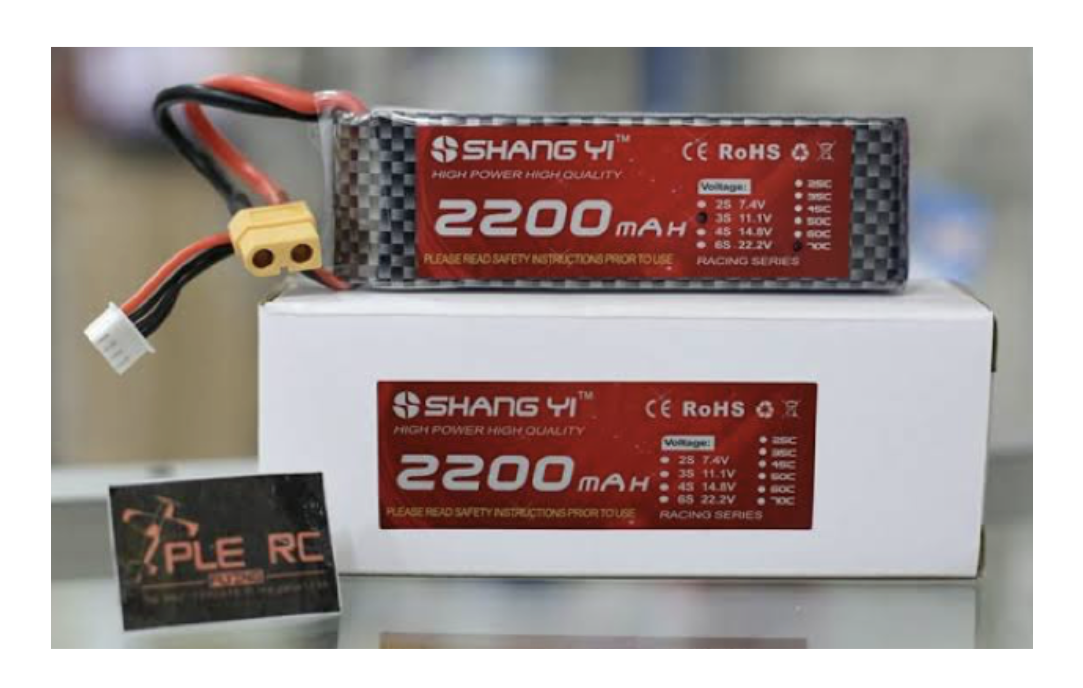
\includegraphics[width=10cm]{./Figures/battery_qc.png}
\caption{Battery (2200mAh 3s, 11V)}
\label{battery_qc}
\end{figure}

\begin{itemize}
    \item Battery Type		: Lithium Polymer 2200mAh 3S 25C
    \item Capacity		: 2200 mAh
    \item Number of cells		: 3S
    \item Total supply voltage	: 11.1V 
    \item Size			: 24 x 34 x 108mm 
    \item Discharge Rate 		: 25 C
    \item Burst Rate 		: 50C
    \item Weight			: 183g 
\end{itemize}

\subsubsection{Overall Interconnection Diagram:}
\begin{figure}[h!]
\centering
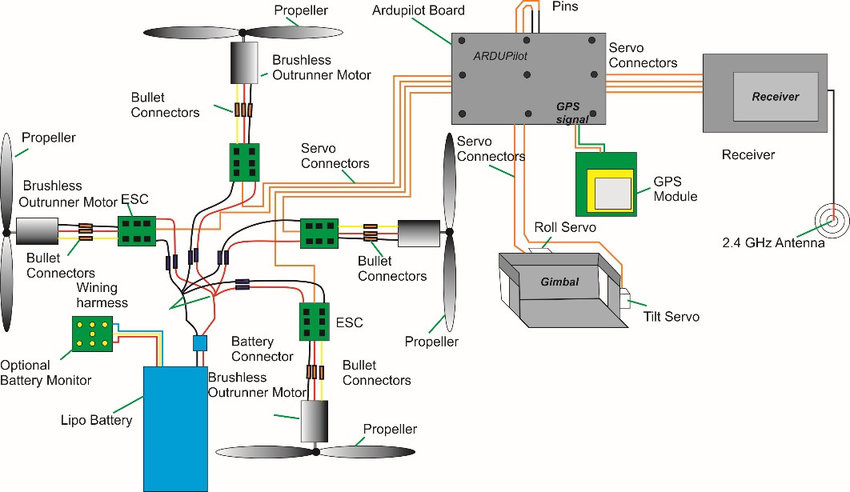
\includegraphics[width=\columnwidth]{./Figures/overall_conn_dia_qc.png}
\caption{Overall Interconnection Diagram for quad-copter}
\label{overall_conn_dia_qc}
\end{figure}

\newpage
\subsubsection{Connection between ESC and motor:}
\begin{figure}[h!]
\centering
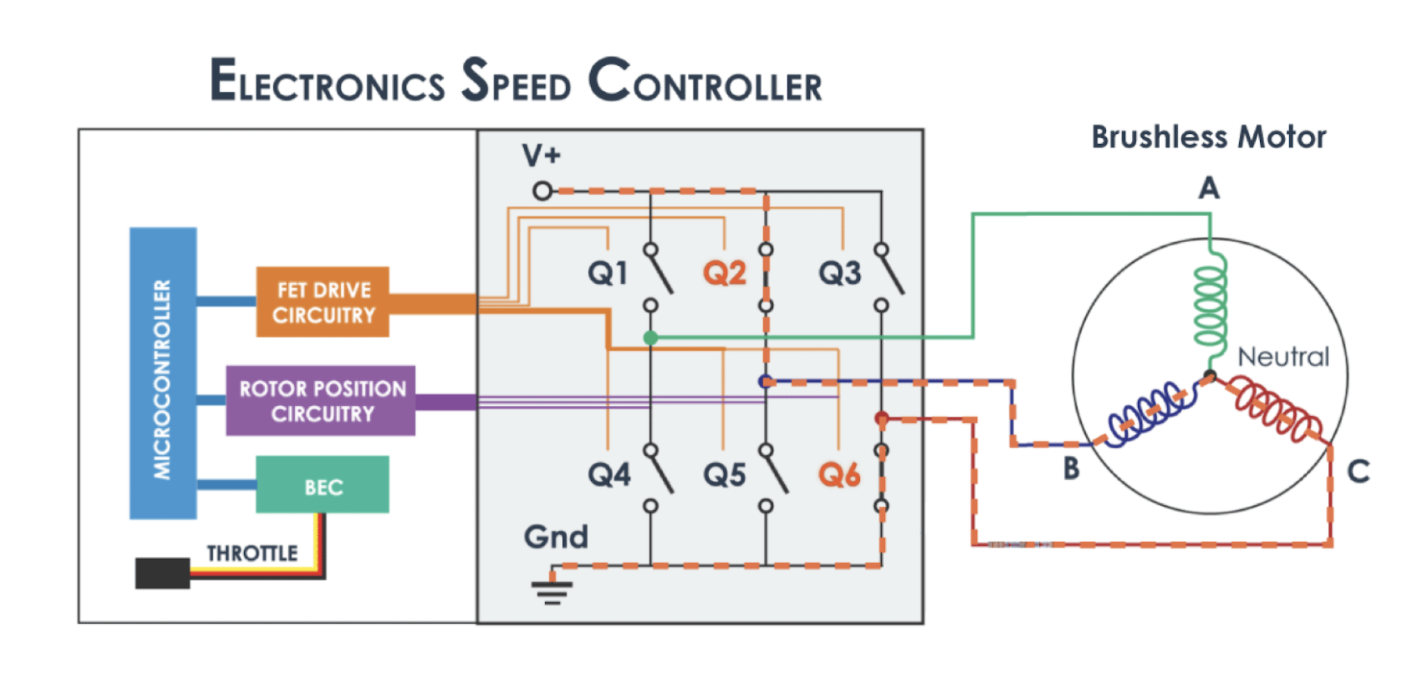
\includegraphics[width=10cm]{./Figures/conn_esc_with_motor_qc.png}
\caption{Connection between ESC and BLDC motor}
\label{conn_esc_with_motor_qc}
\end{figure}

\subsubsection{PWM signal from Controller to ESC:}
\begin{figure}[h!]
\centering
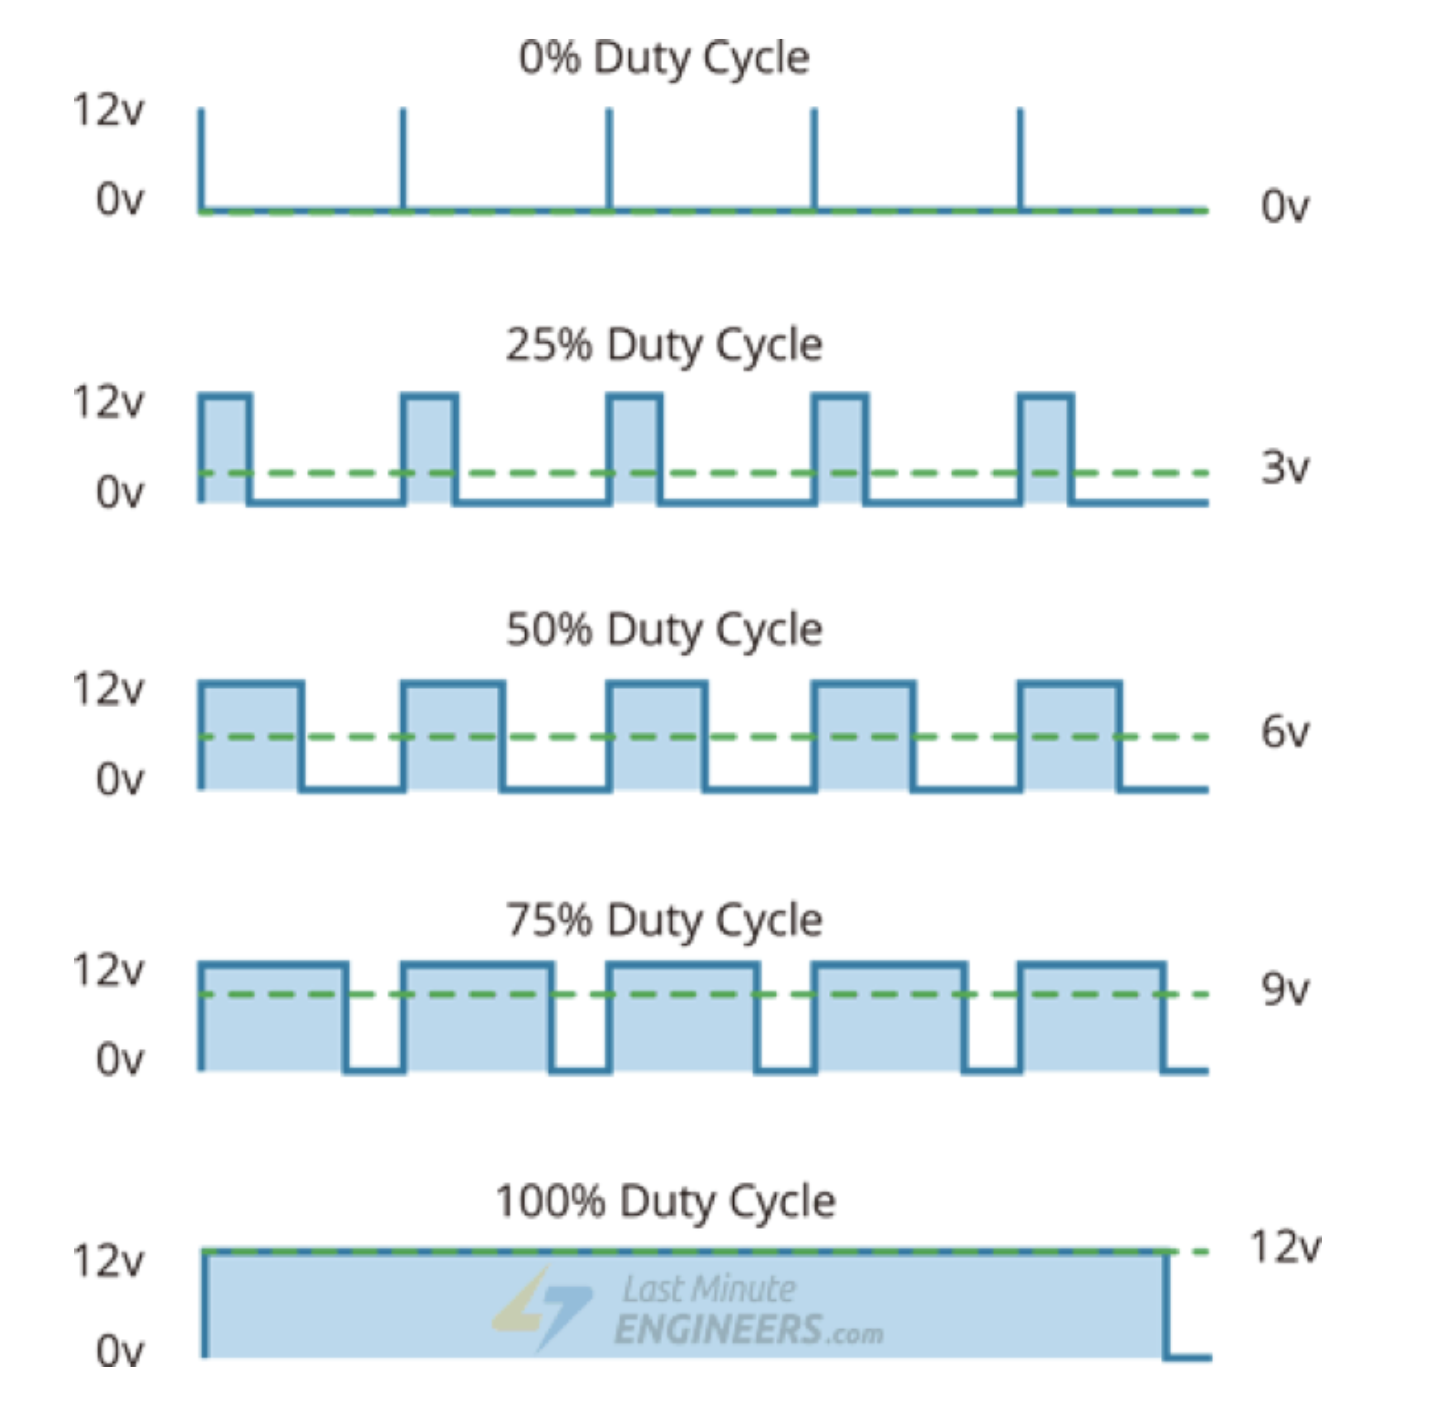
\includegraphics[width=9cm]{./Figures/signal_from_controller2esc_qc.png}
\caption{PWM signal from Controller to ESC:}
\label{signal_from_controller2esc_qc}
\end{figure}

\begin{itemize}
    \item PWM Signal is sent from the controller to the ESC module in order to control the speed of the motor.
    \item Lesser the Duty cycle of the PWM signal, lesser is the RPM of the motor.
    \item Max. RPM achieved at 100\% Duty cycle. 
\end{itemize}


\subsection{Configuration of Drone}
\subsubsection{All files and resources related to configuration can be found at below GitHub link} 
\begin{tcolorbox}
        \url{https://github.com/Abhishek-IITH/Drone-Building.git}
\end{tcolorbox}
\subsubsection{Installing Mission planner on UBUNTU 20.04}
\textbf{STEP 1: Install Mono}
\begin{lstlisting}
sudo apt install mono-runtime libmono-system-windows-forms4.0-cil libmono-system-core4.0-cil libmono-winforms2.0-cil libmono-corlib2.0-cil libmono-system-management4.0-cil libmono-system-xml-linq4.0-cil
\end{lstlisting}
OR full Mono: (In case the upper command does not work use this one.)
\begin{lstlisting}
sudo apt install mono-complete
\end{lstlisting}
\\
\textbf{STEP 2: Download Mission planner}
Download MissionPlanner.zip using the below steps:
\begin{itemize}
    \item Get the latest zipped version of Mission planner here:
    \begin{tcolorbox}
        \url{https://firmware.ardupilot.org/Tools/MissionPlanner/MissionPlanner-latest.zip}
    \end{tcolorbox}
    \item Unzip in the appropriate directory
    \item Open terminal, go into the directory where you unzipped your mission planner.
    \item Run Mission planner using the command:
    \begin{lstlisting}
        mono MissionPlanner.exe.
    \end{lstlisting}
\end{itemize}
You can debug Mission Planner on Mono with the command:
\begin{lstlisting}
MONO_LOG_LEVEL=debug mono MissionPlanner.exe
\end{lstlisting}

\newpage

\begin{figure}[h!]
\centering
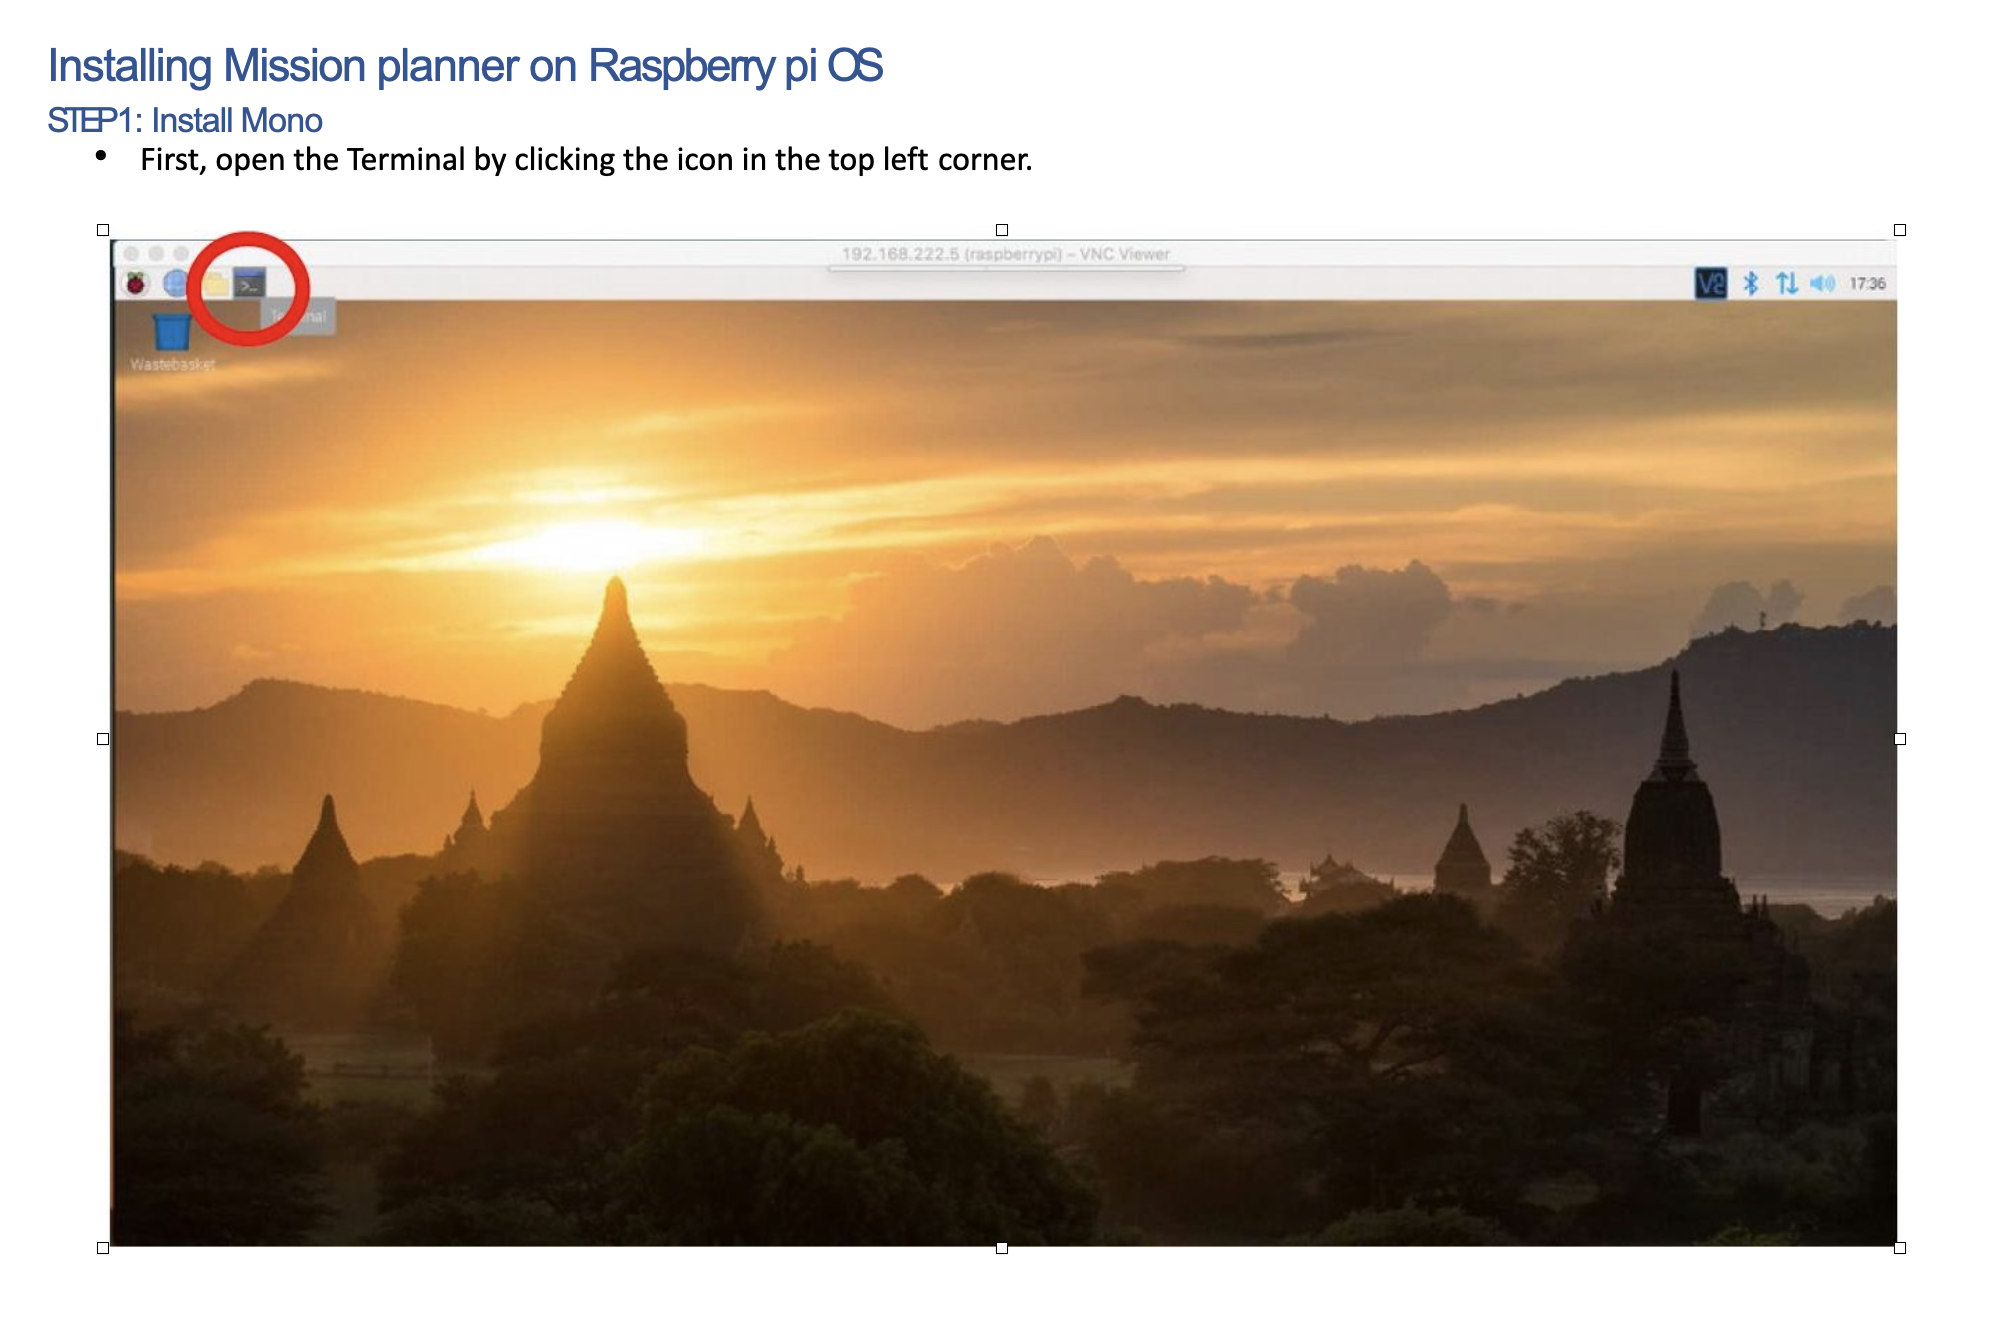
\includegraphics[width=\columnwidth]{./Figures/config_img1_qc.png}
\end{figure}

\begin{figure}[h!]
\centering
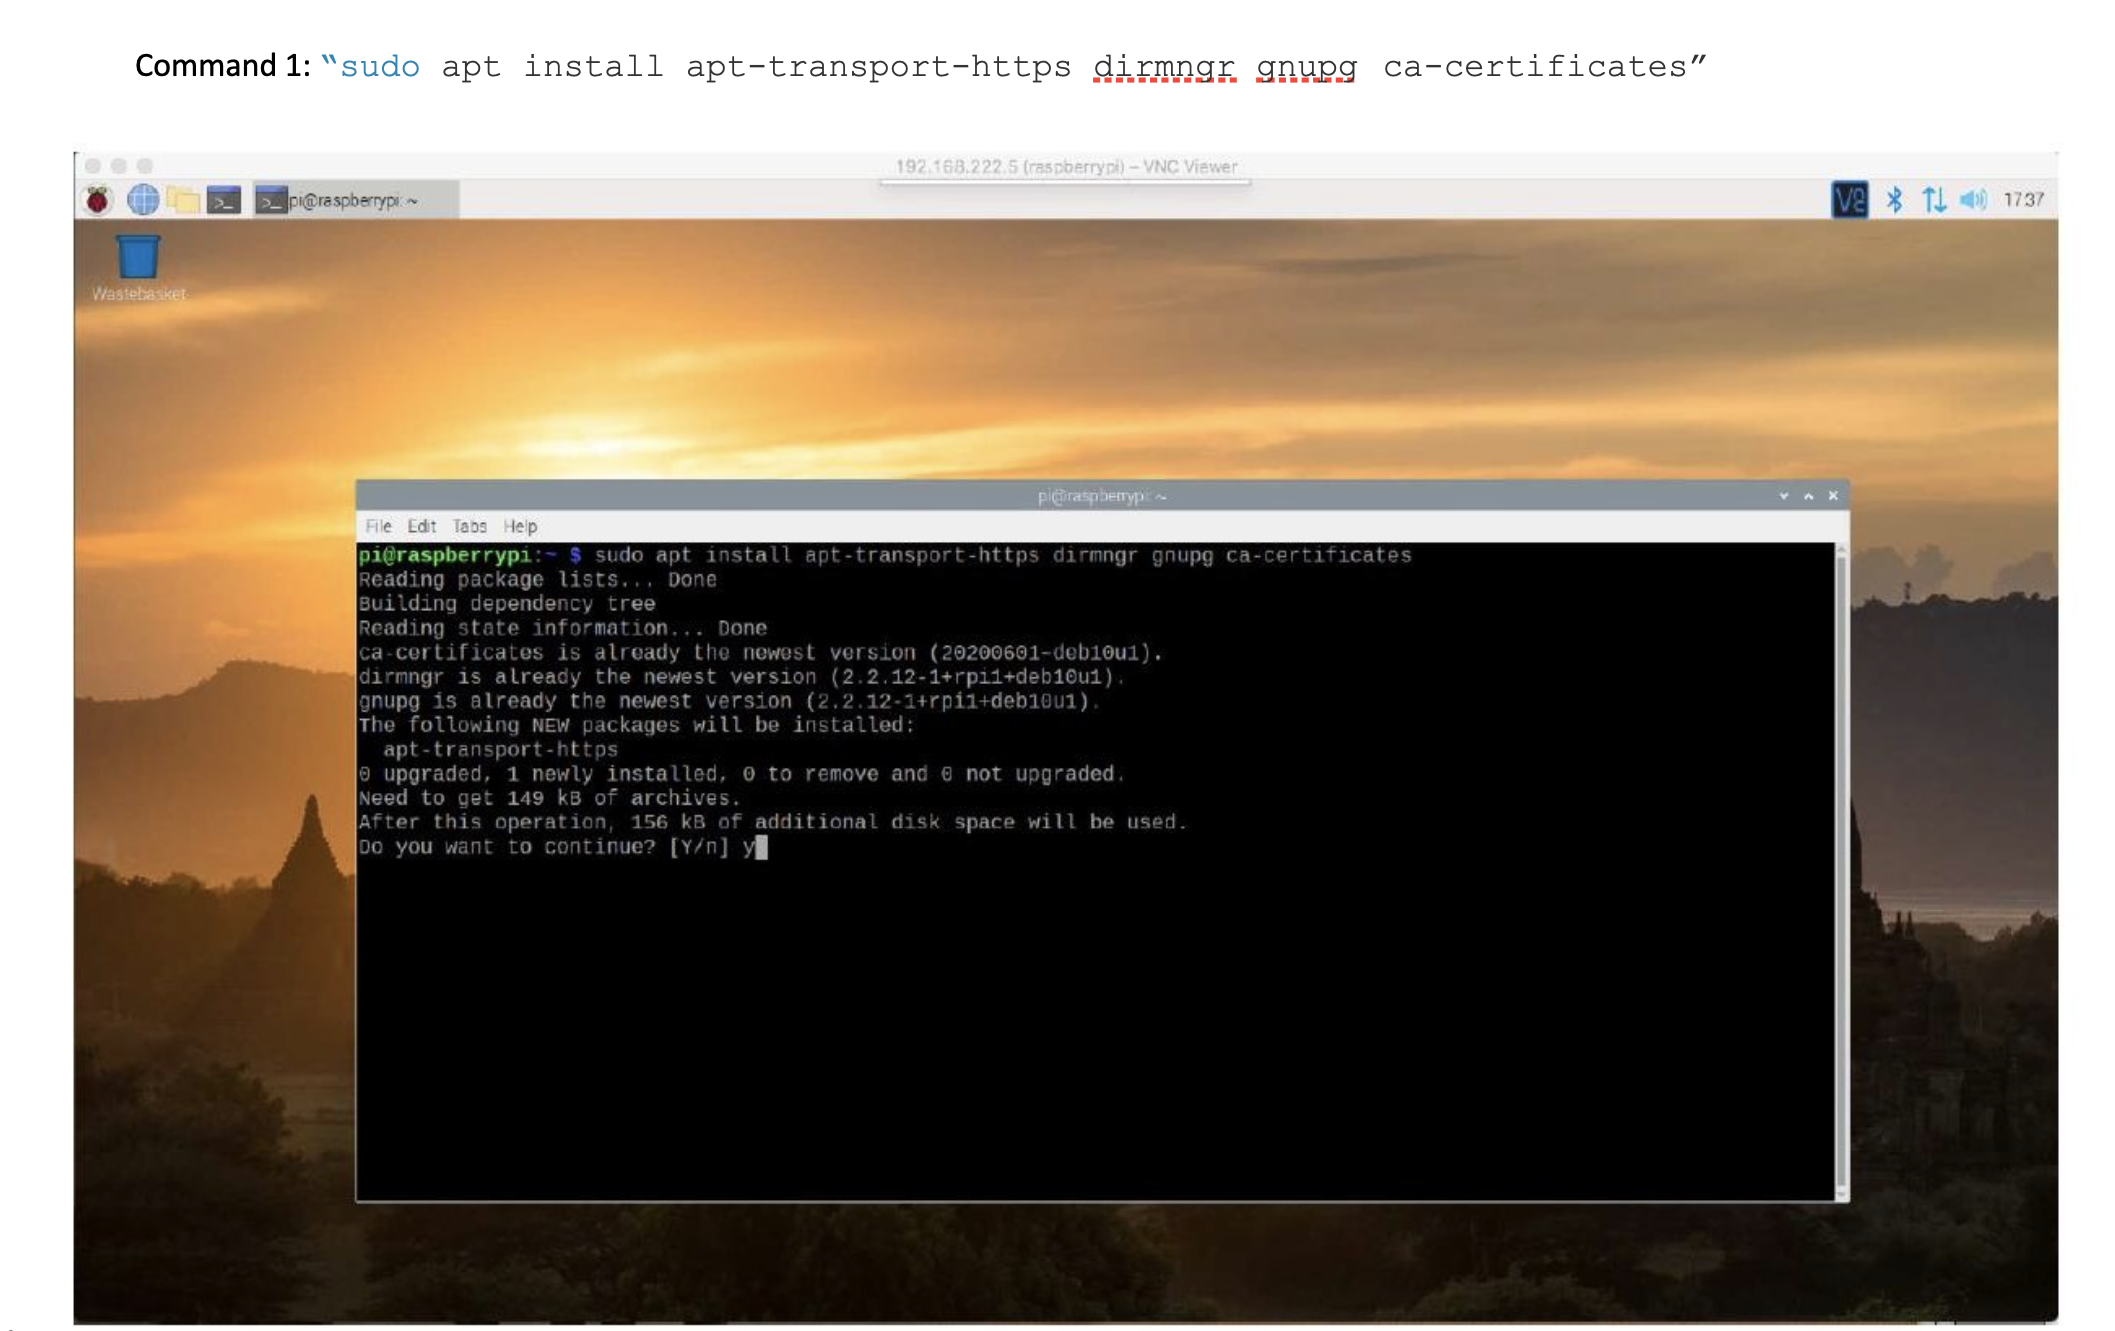
\includegraphics[width=\columnwidth]{./Figures/config_img2.png}
\end{figure}

\begin{figure}[h!]
\centering
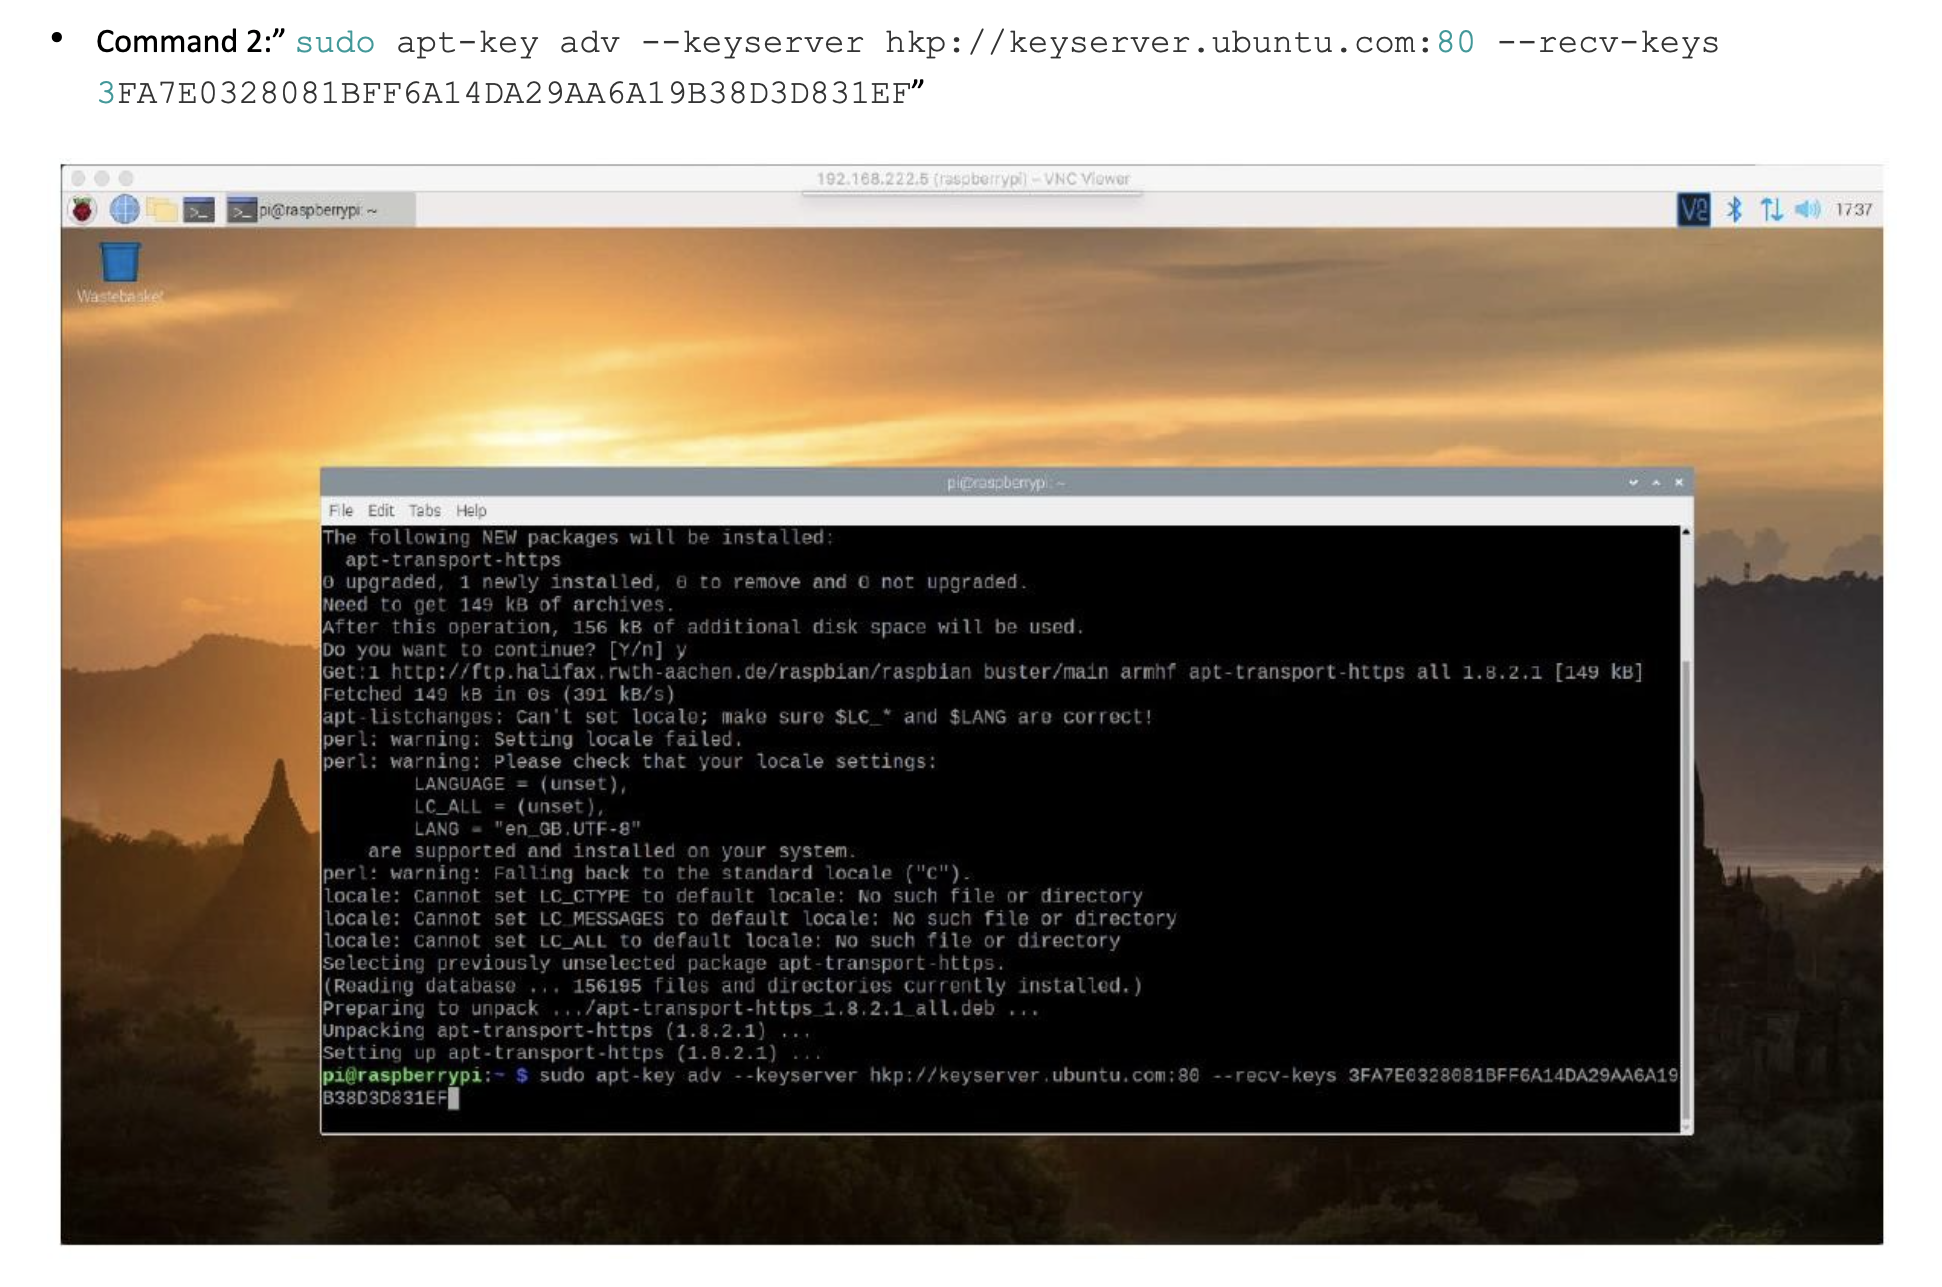
\includegraphics[width=\columnwidth]{./Figures/config_img3.png}
\end{figure}

\begin{figure}[h!]
\centering
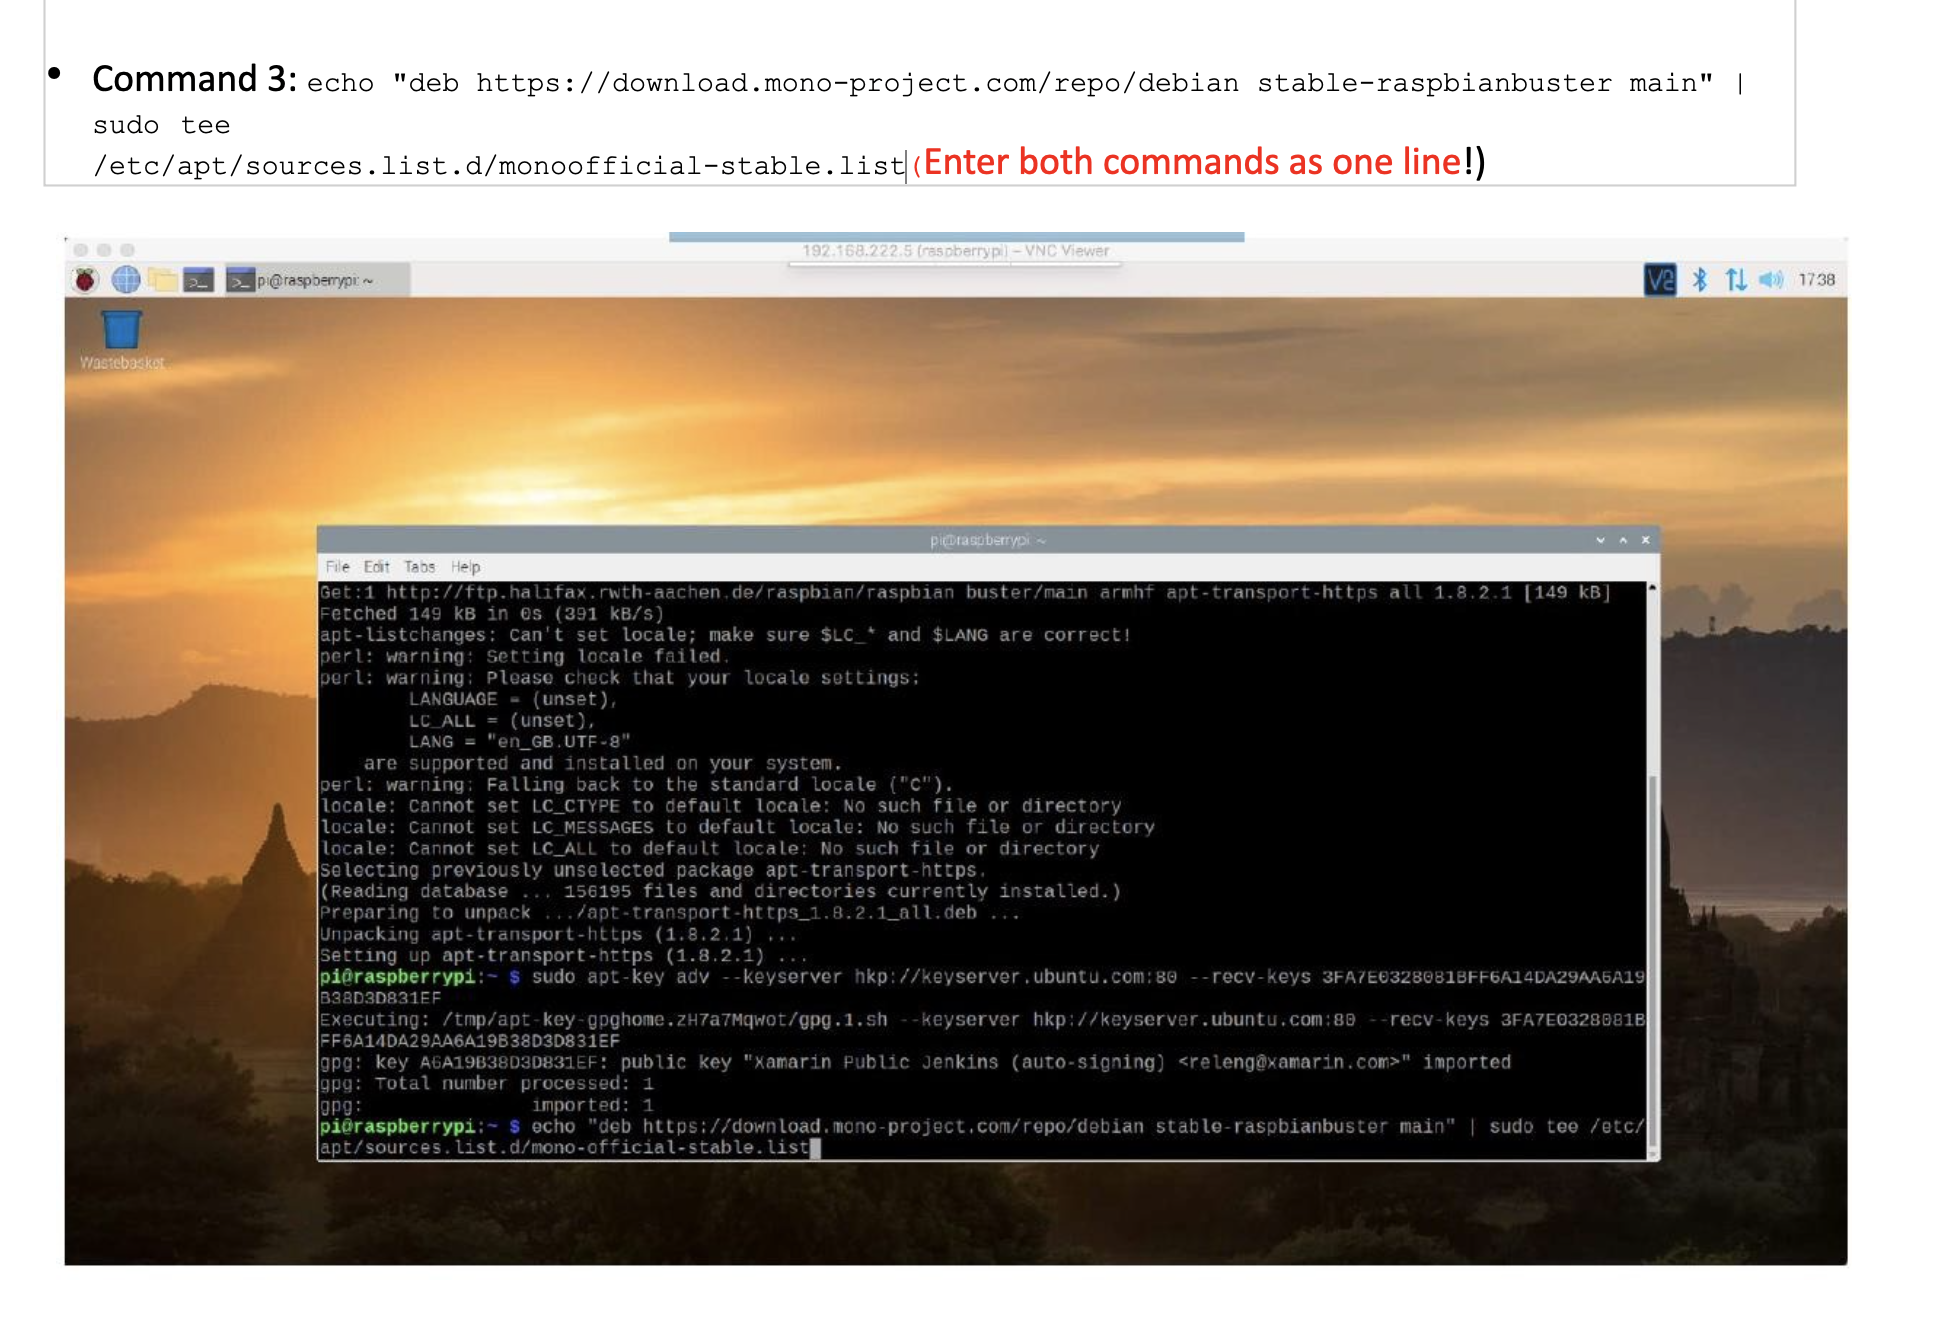
\includegraphics[width=\columnwidth]{./Figures/config_img4.png}
\end{figure}

\begin{figure}[h!]
\centering
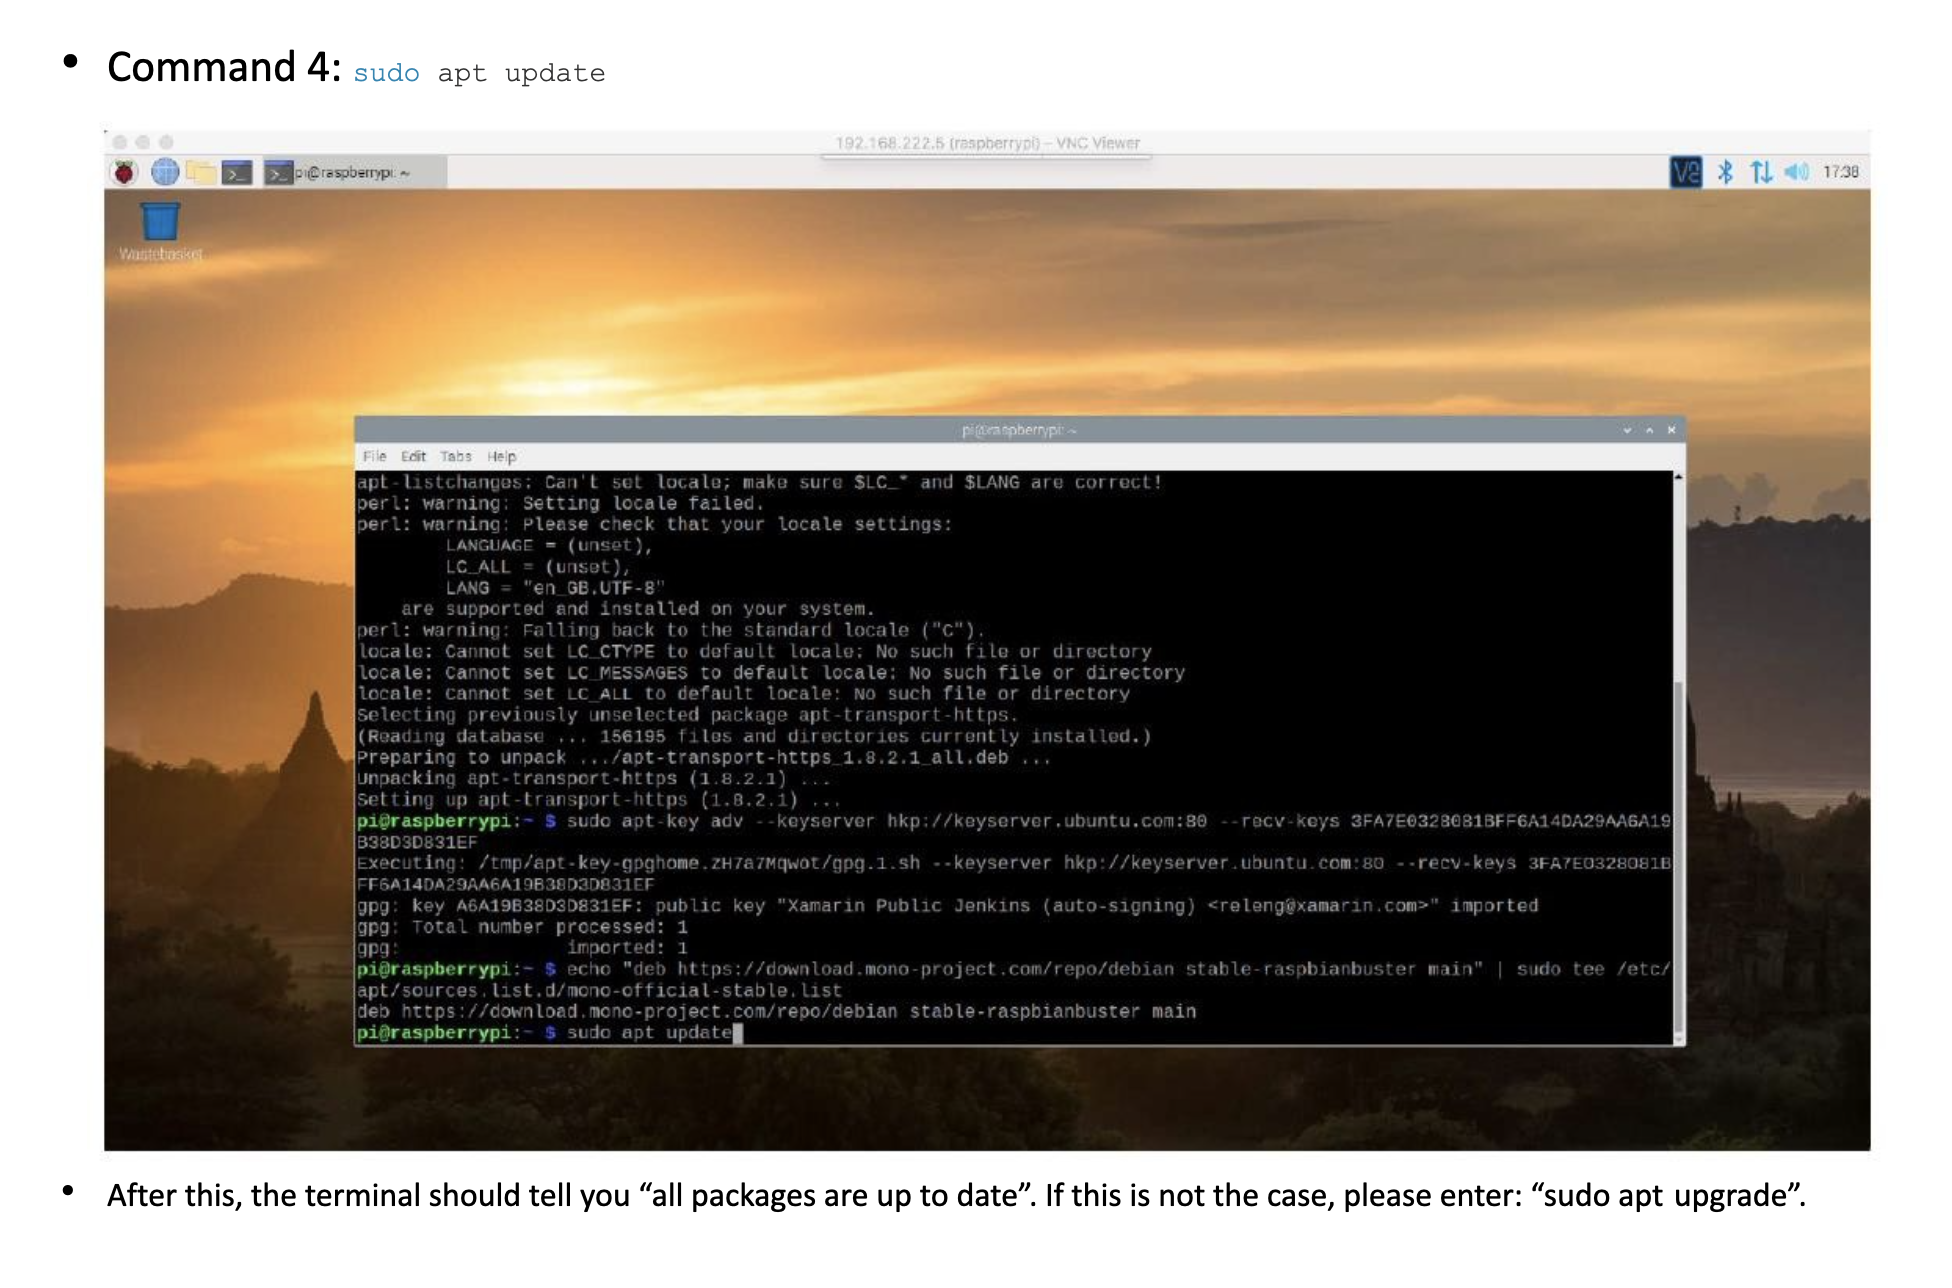
\includegraphics[width=\columnwidth]{./Figures/config_img5.png}
\end{figure}

\begin{figure}[h!]
\centering
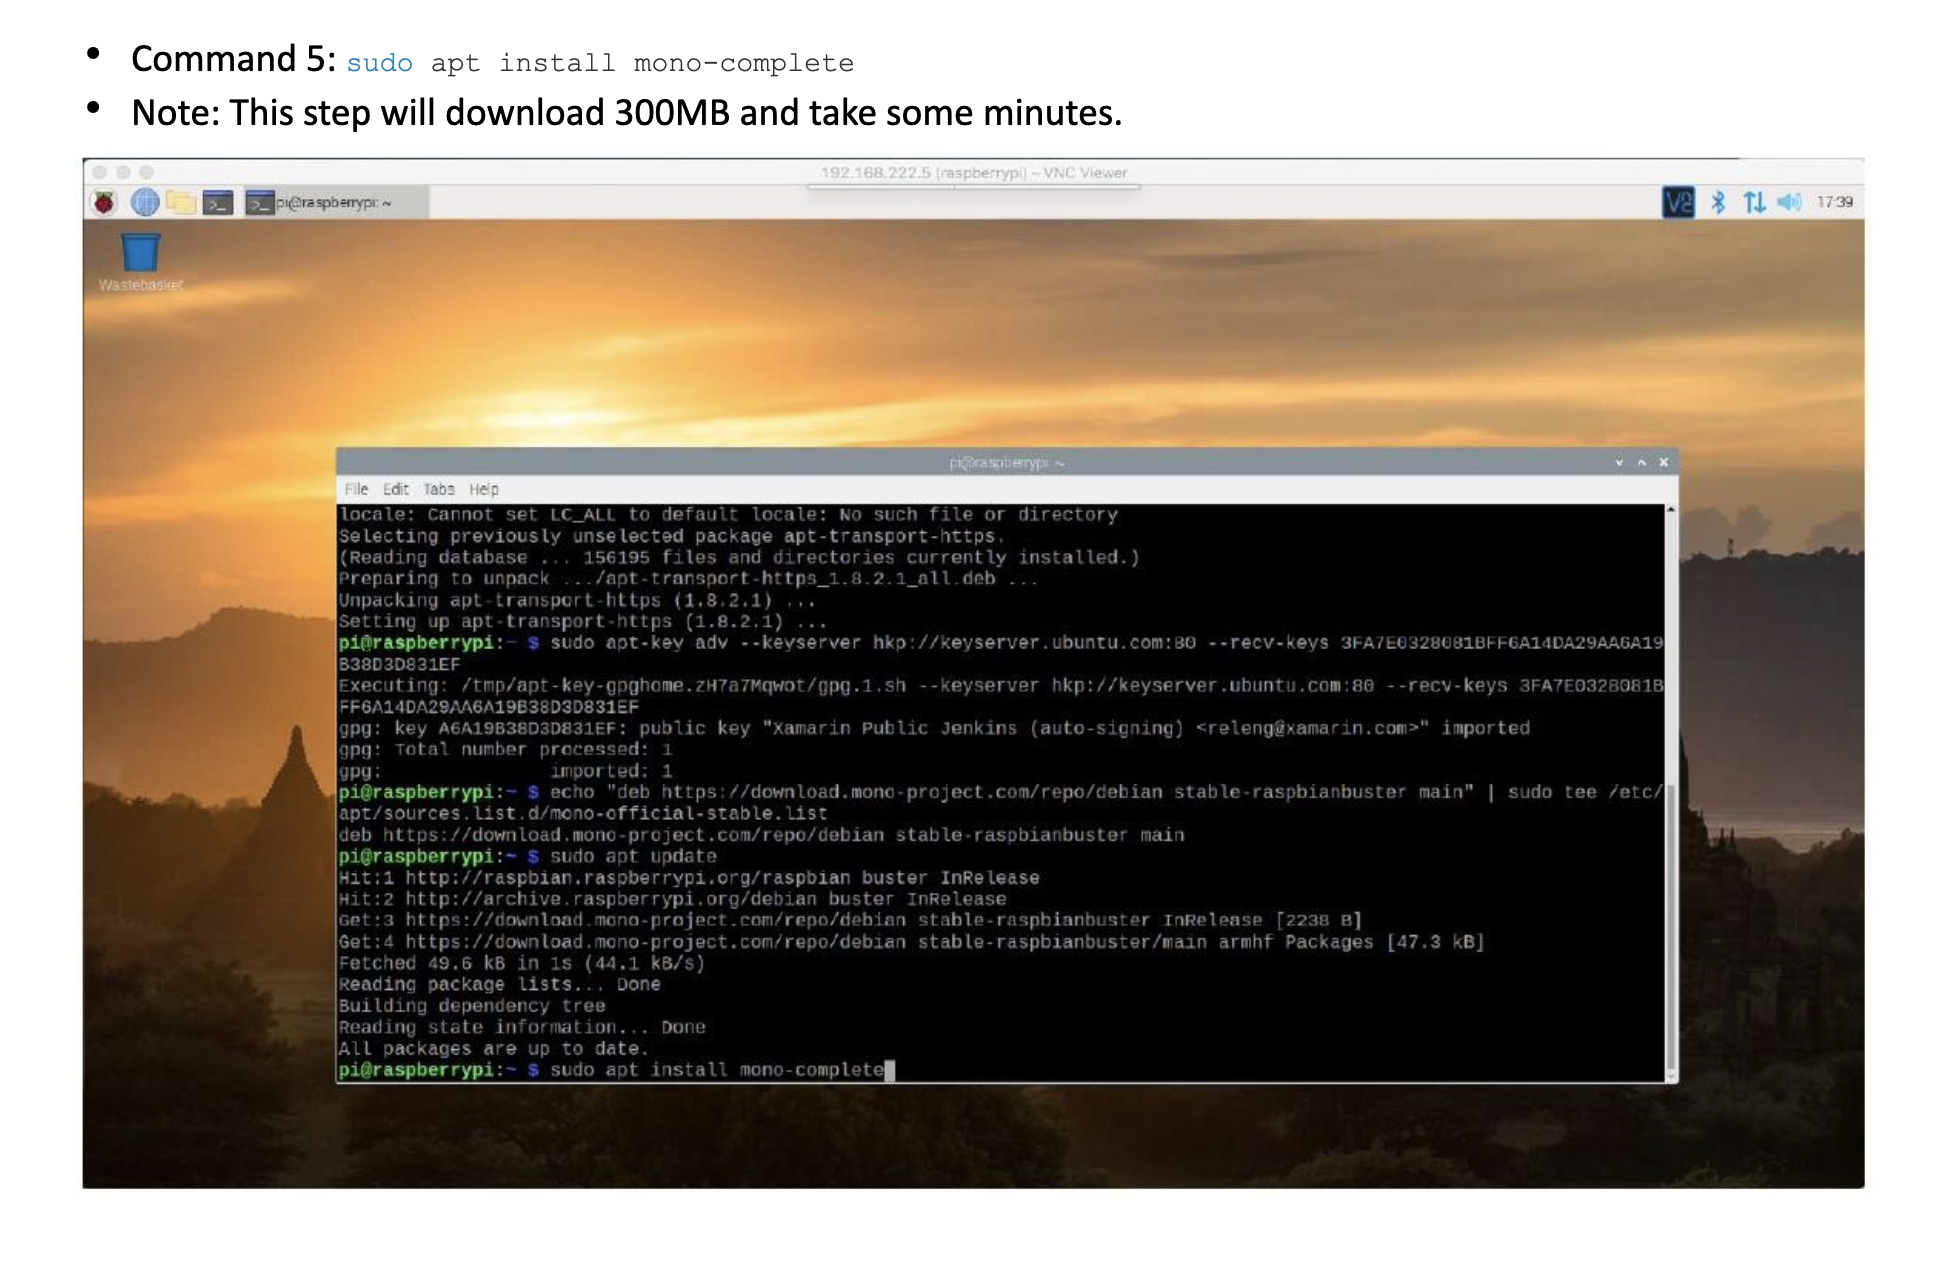
\includegraphics[width=\columnwidth]{./Figures/config_img6.png}
\end{figure}

\begin{figure}[h!]
\centering
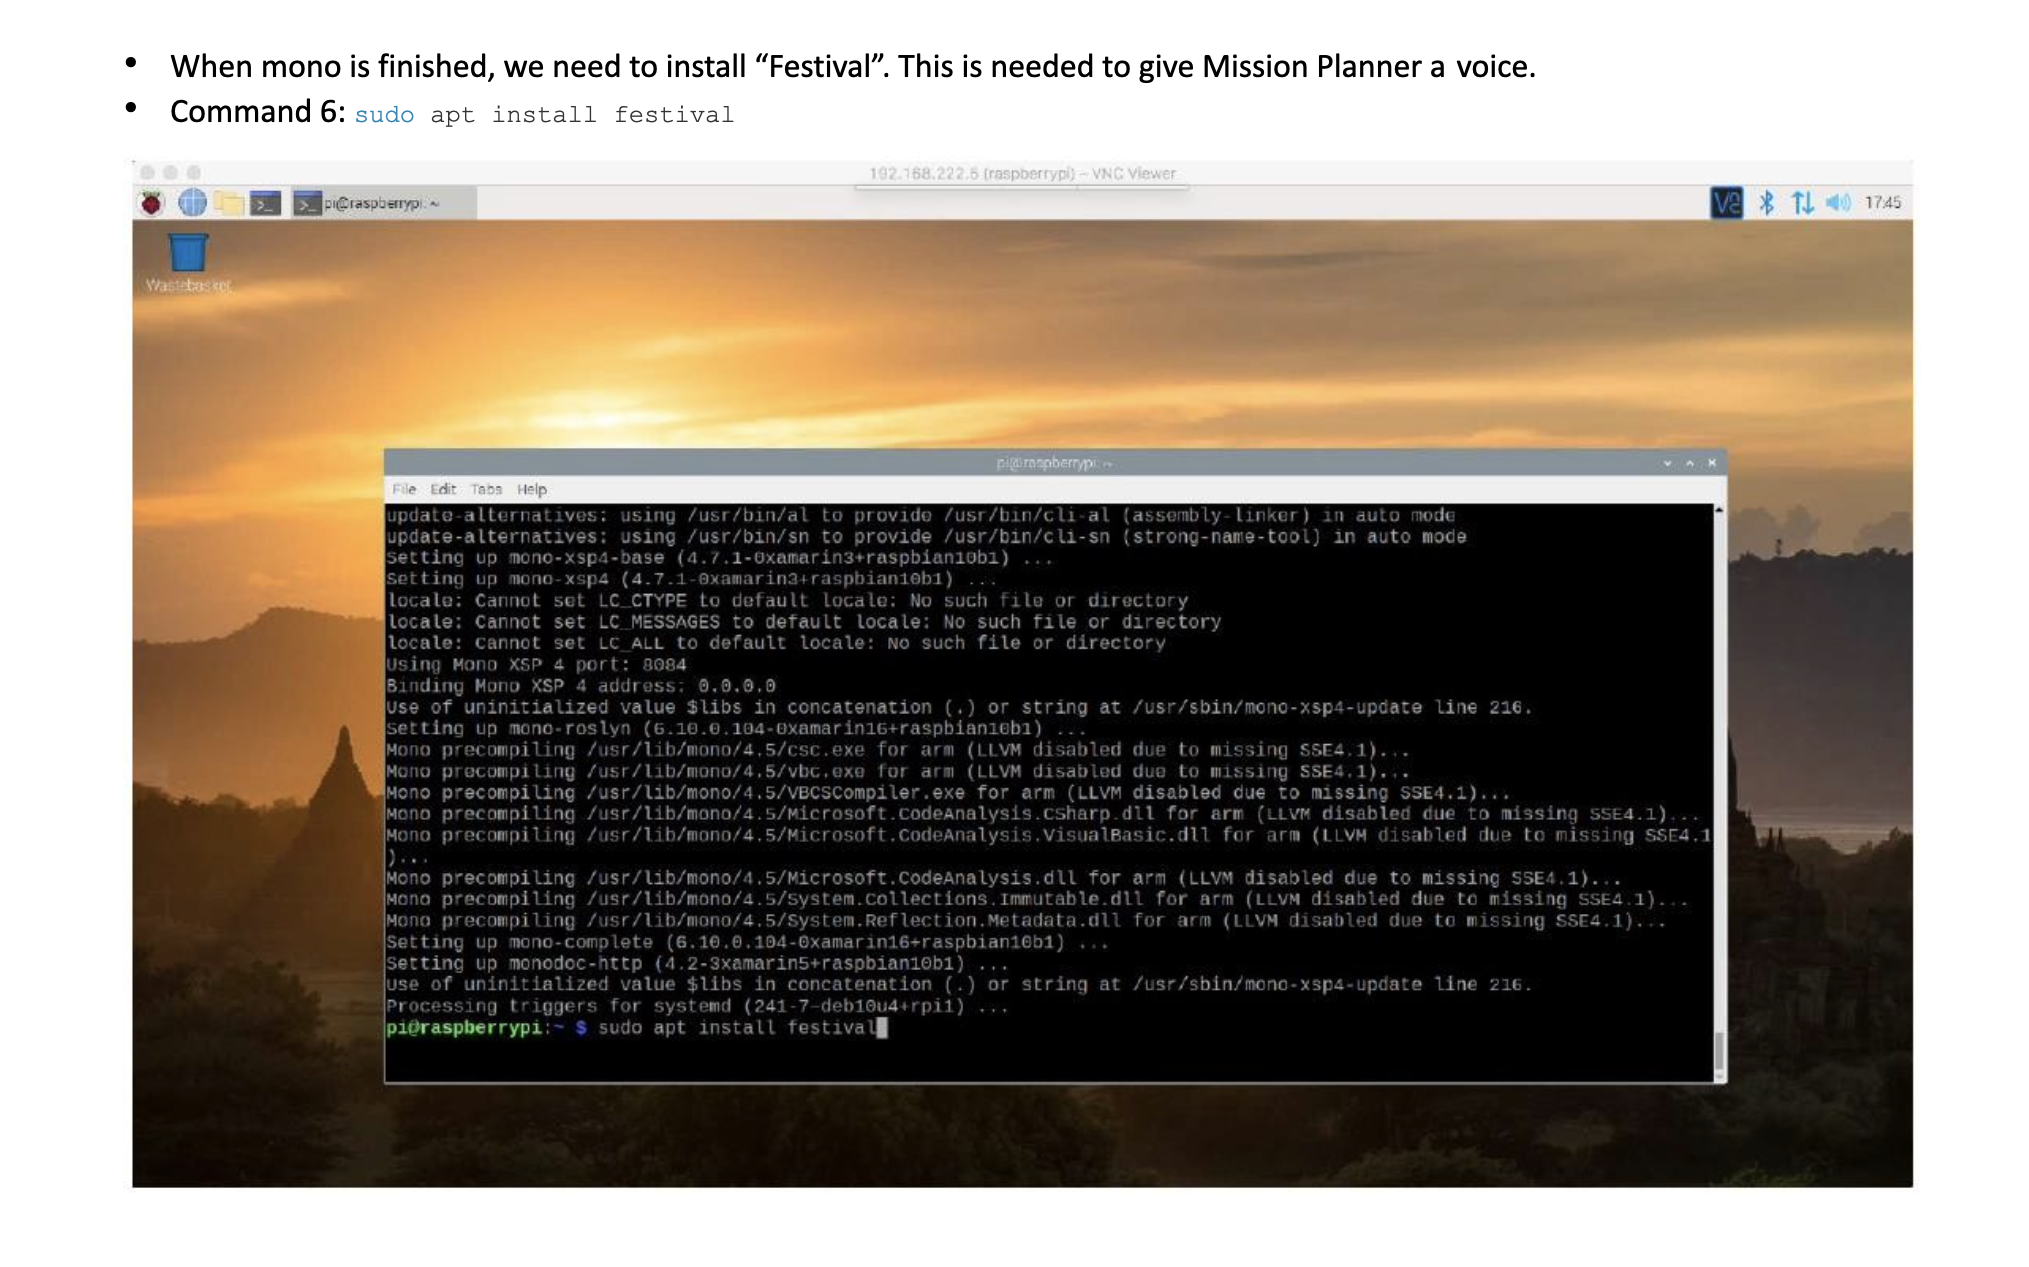
\includegraphics[width=\columnwidth]{./Figures/config_img7.png}
\end{figure}

\begin{figure}[h!]
\centering
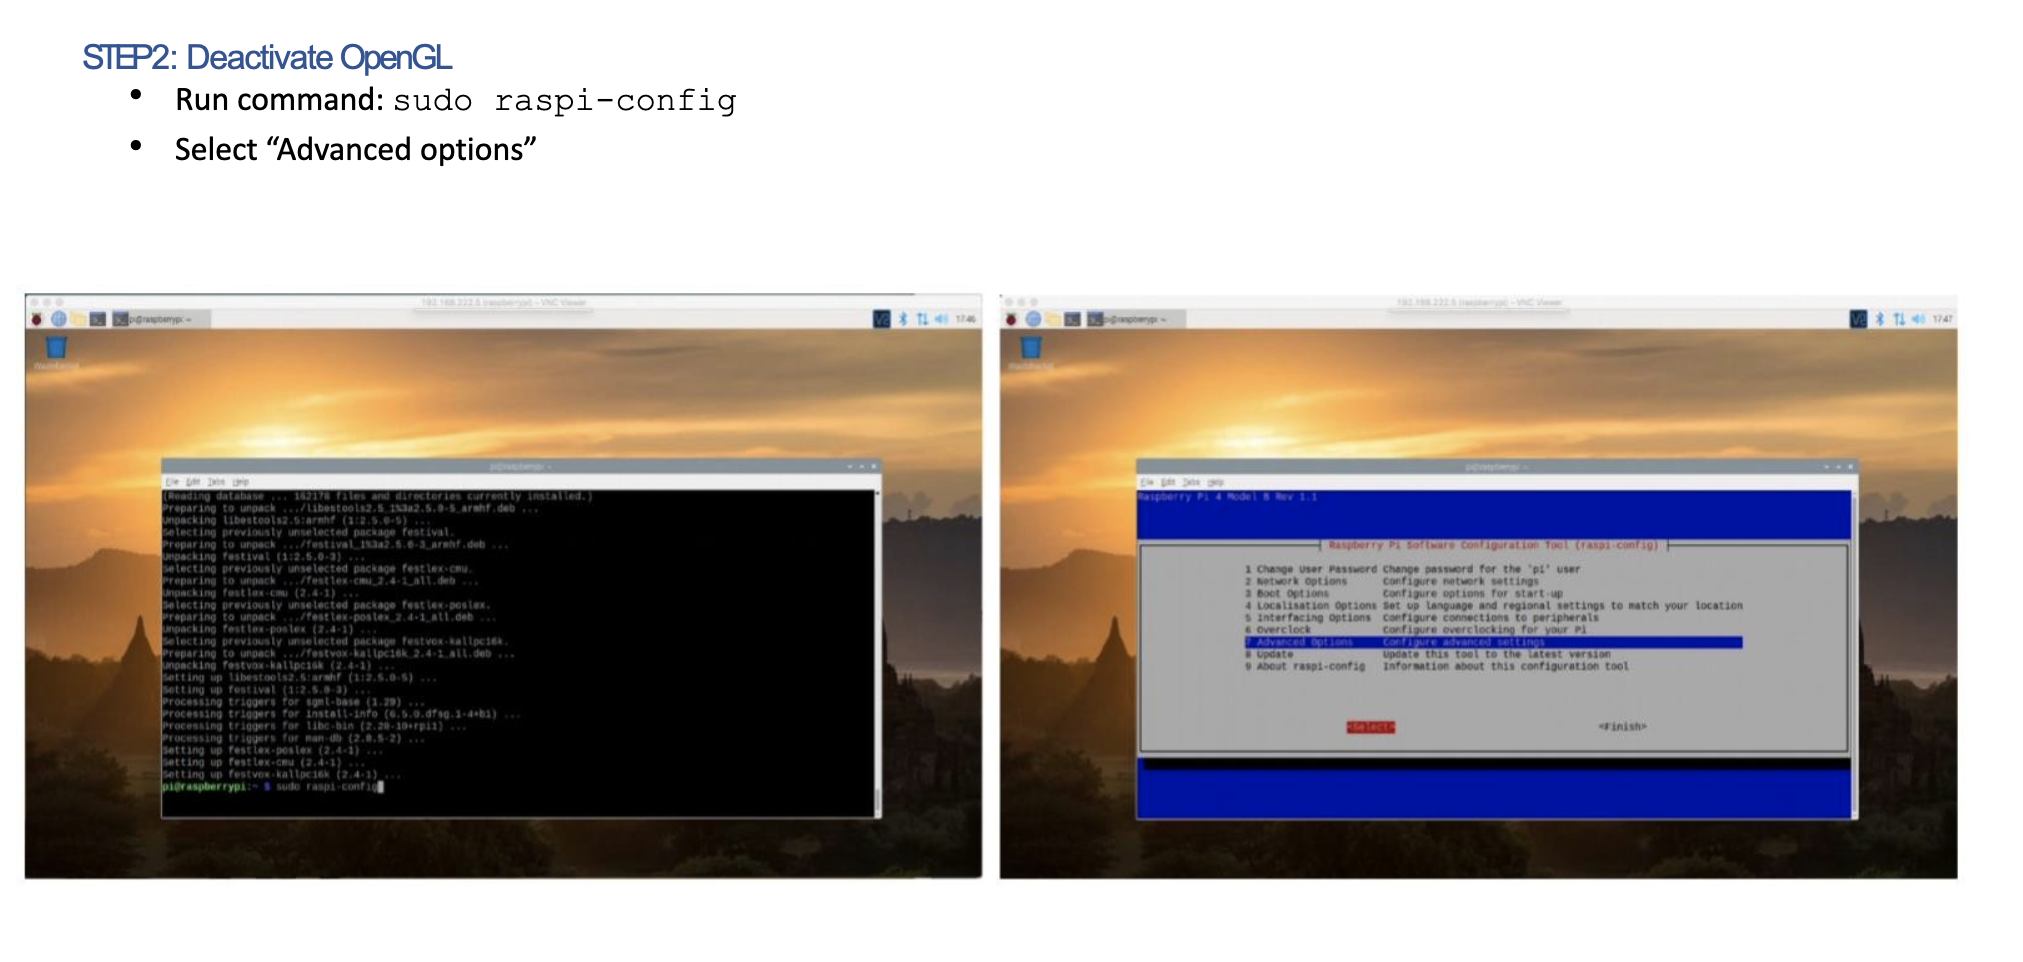
\includegraphics[width=\columnwidth]{./Figures/config_img8.png}
\end{figure}

\begin{figure}[h!]
\centering
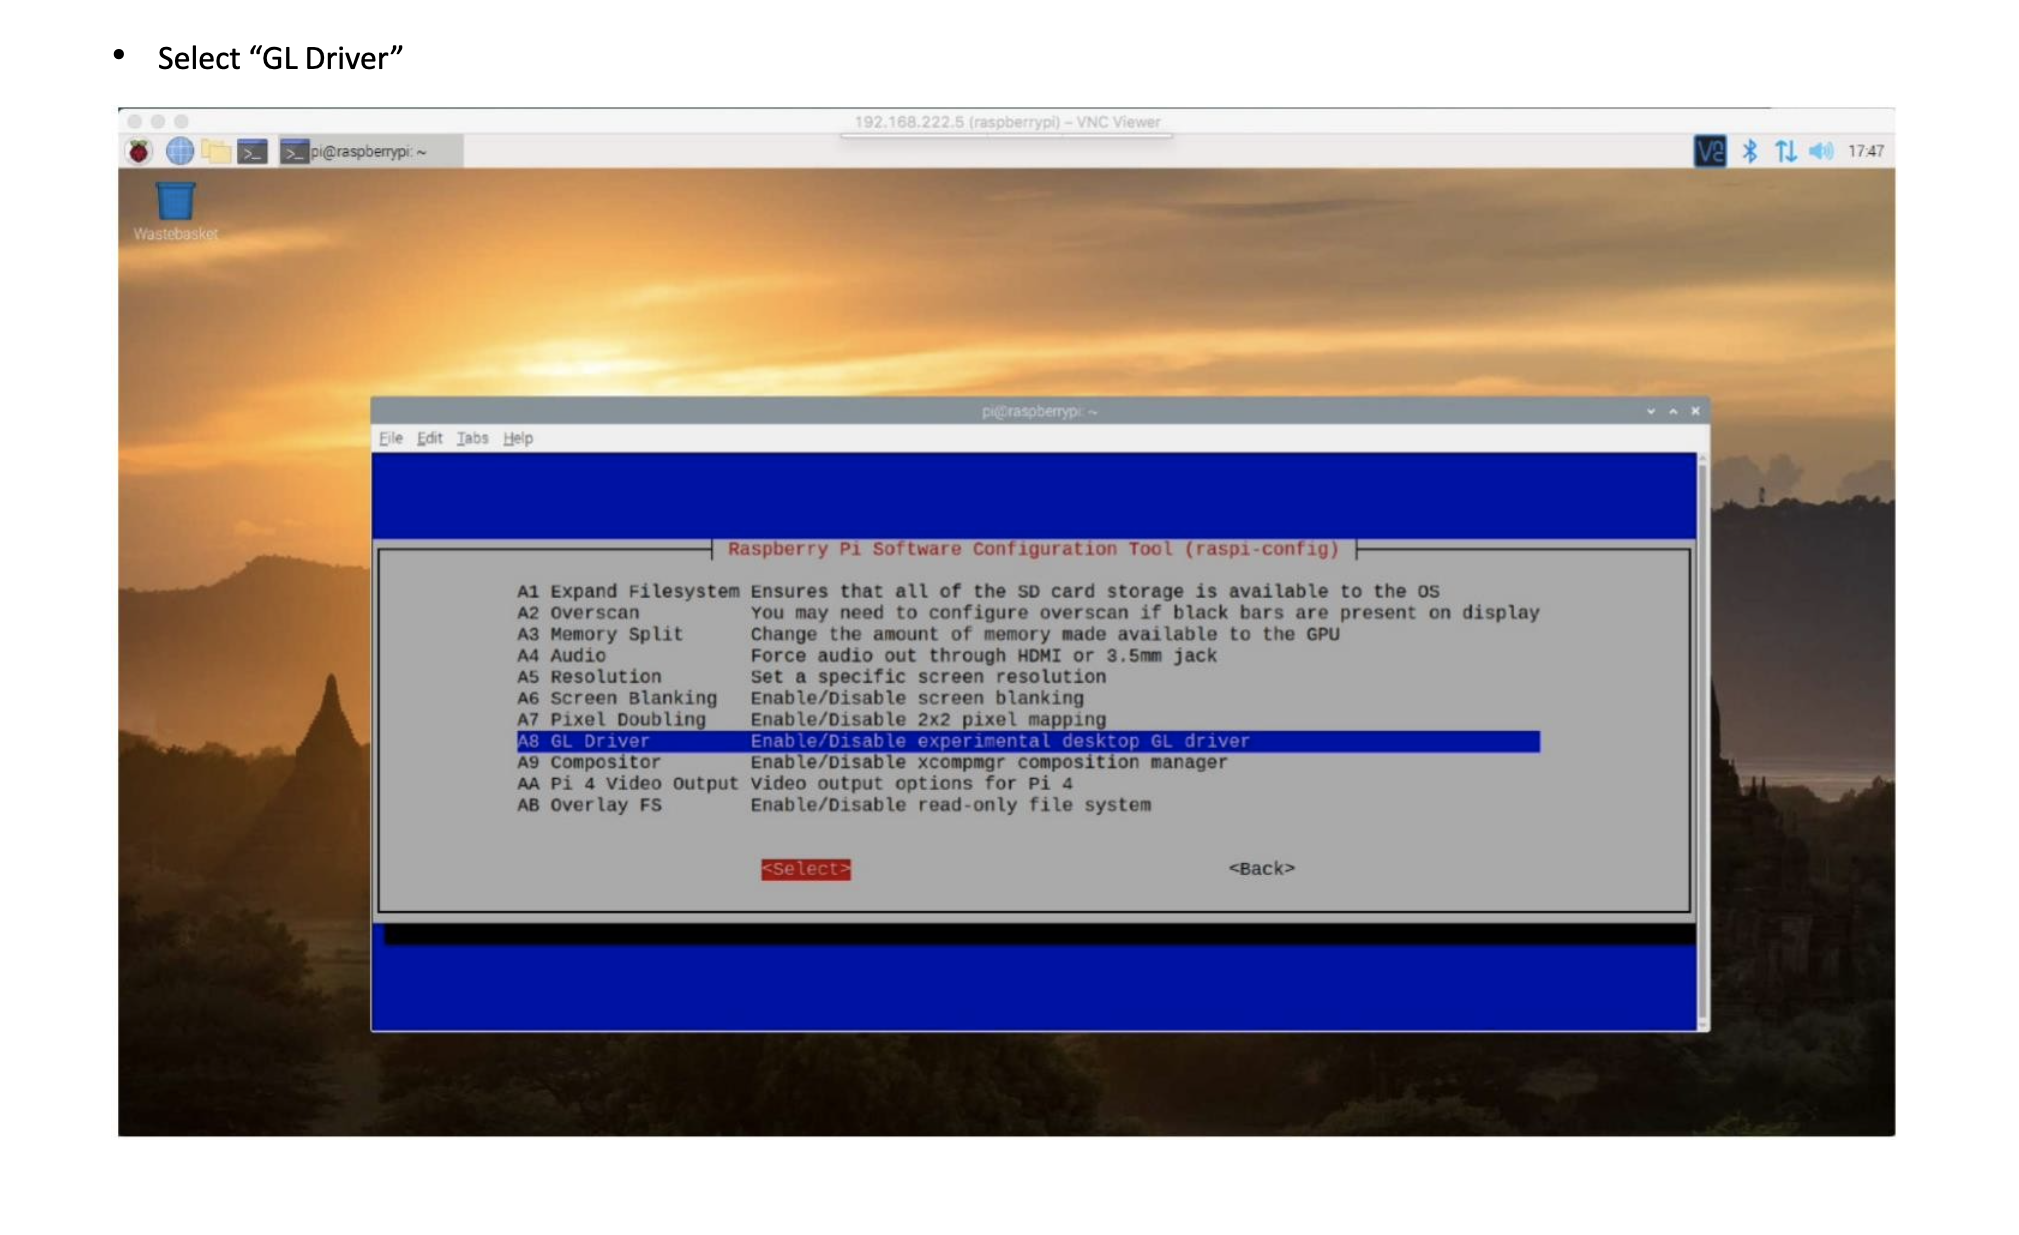
\includegraphics[width=\columnwidth]{./Figures/config_img9.png}
\end{figure}

\begin{figure}[h!]
\centering
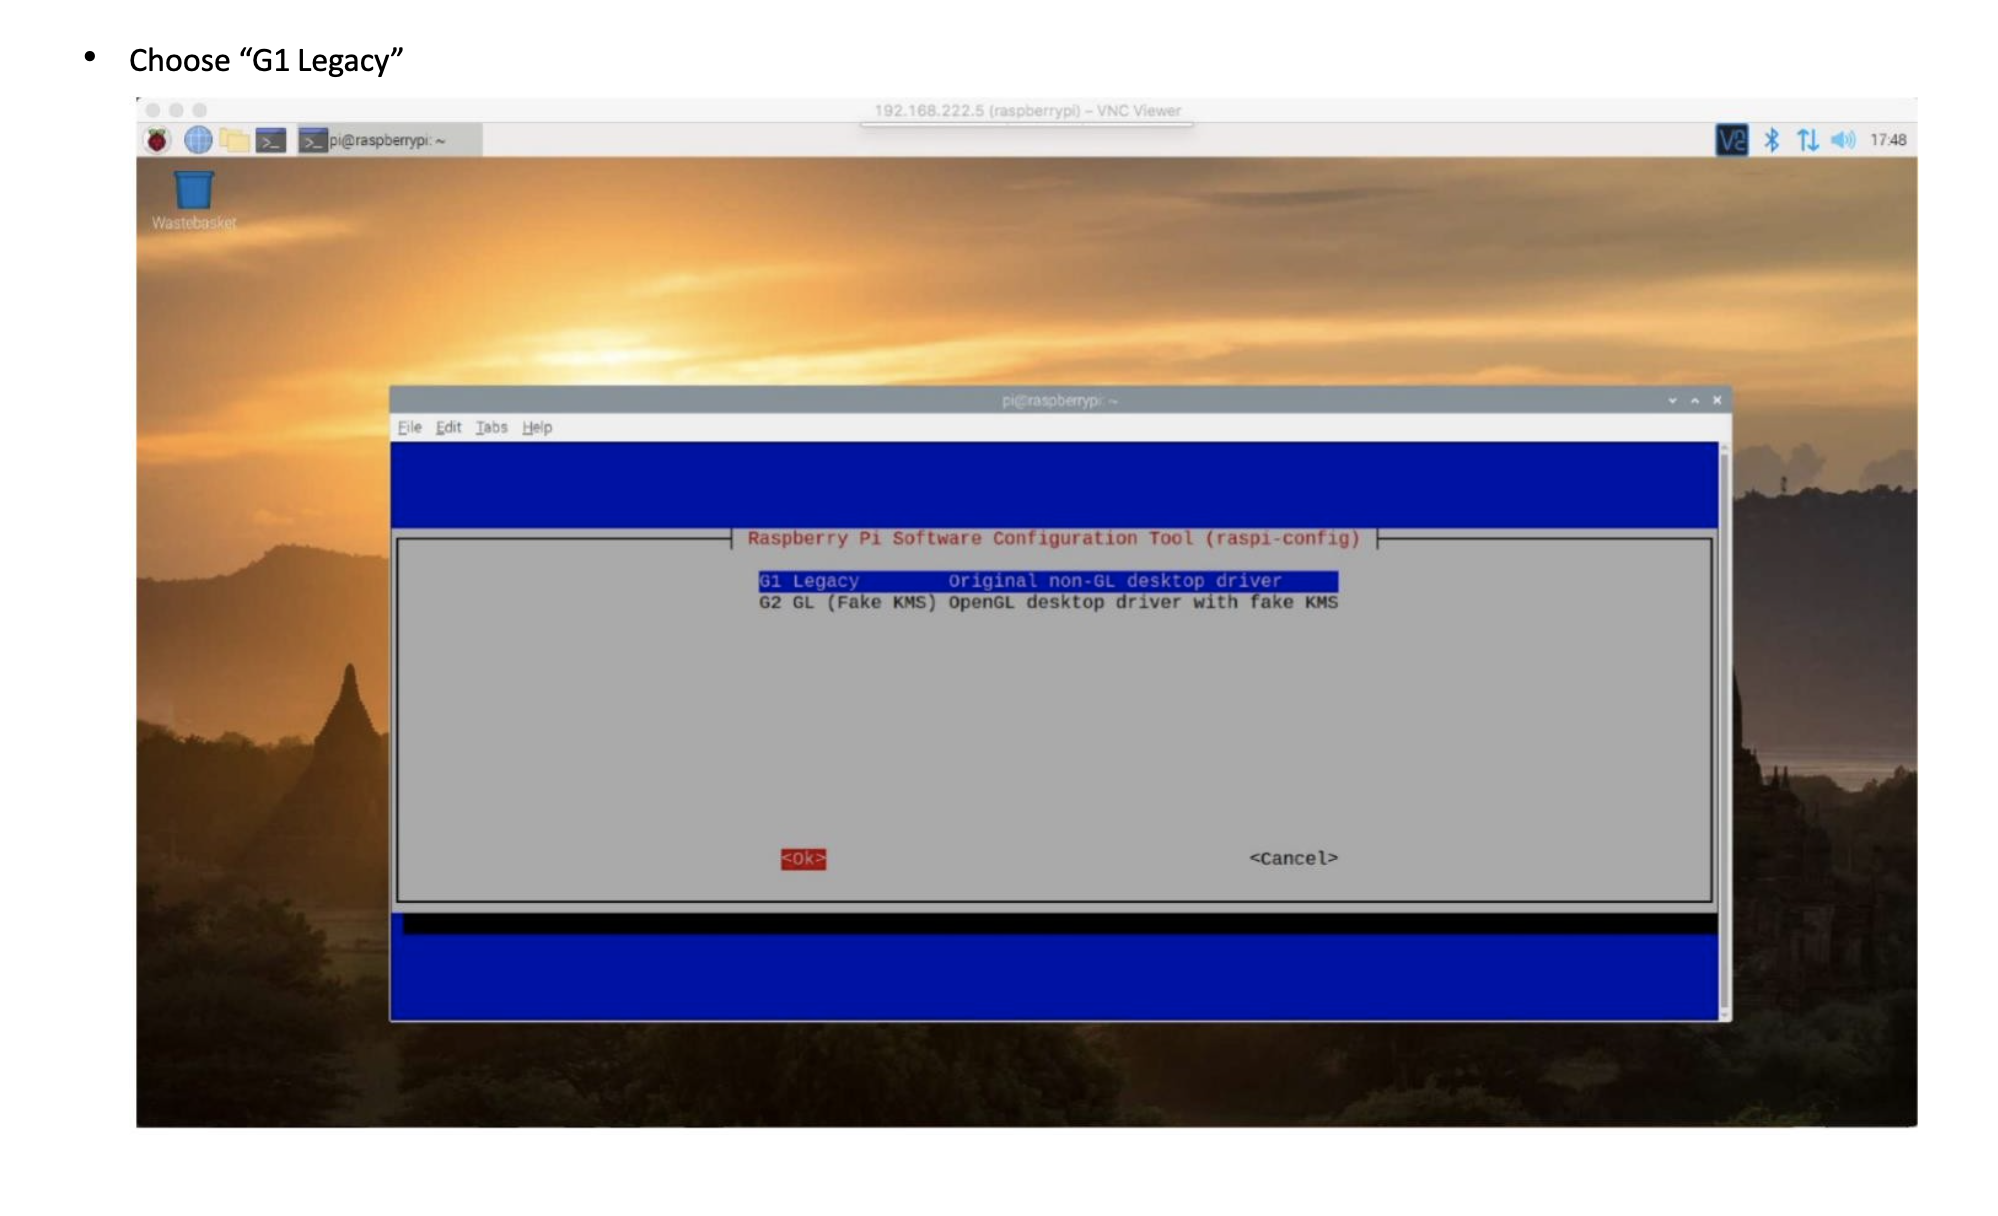
\includegraphics[width=\columnwidth]{./Figures/config_img10.png}
\end{figure}

\begin{figure}[h!]
\centering
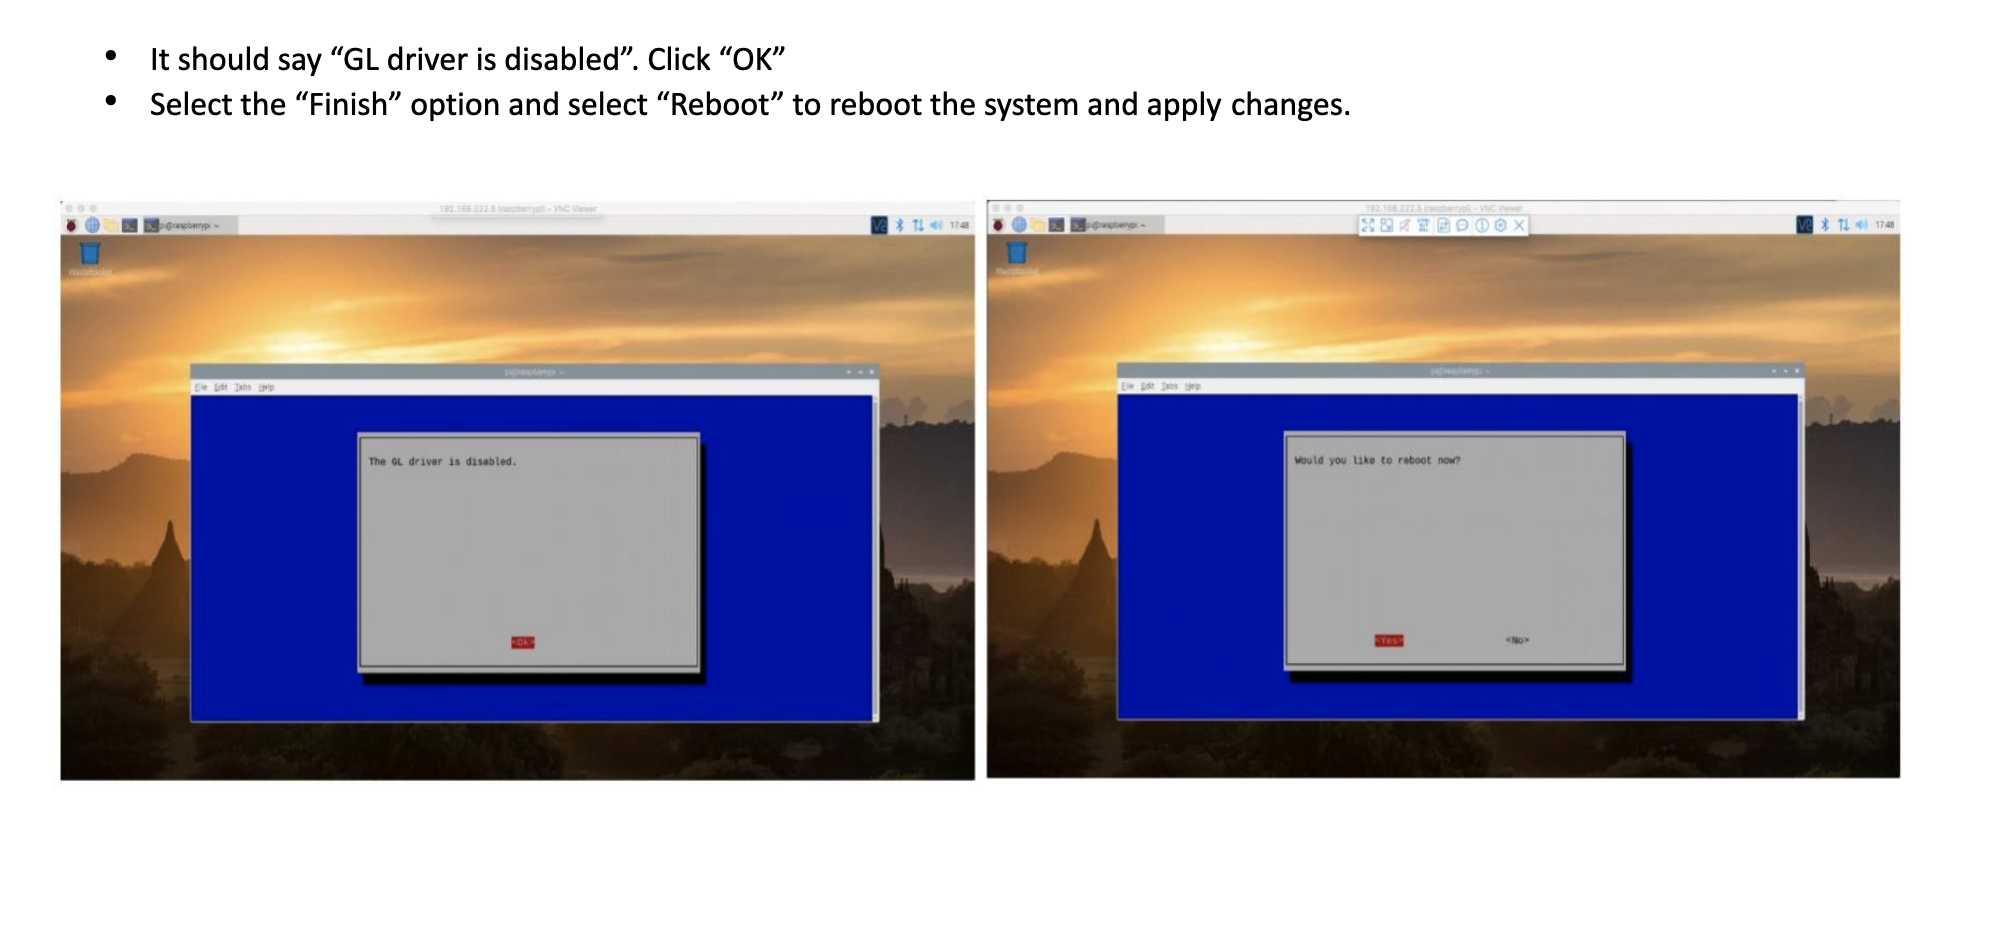
\includegraphics[width=\columnwidth]{./Figures/config_img11.png}
\end{figure}

\begin{figure}[h!]
\centering
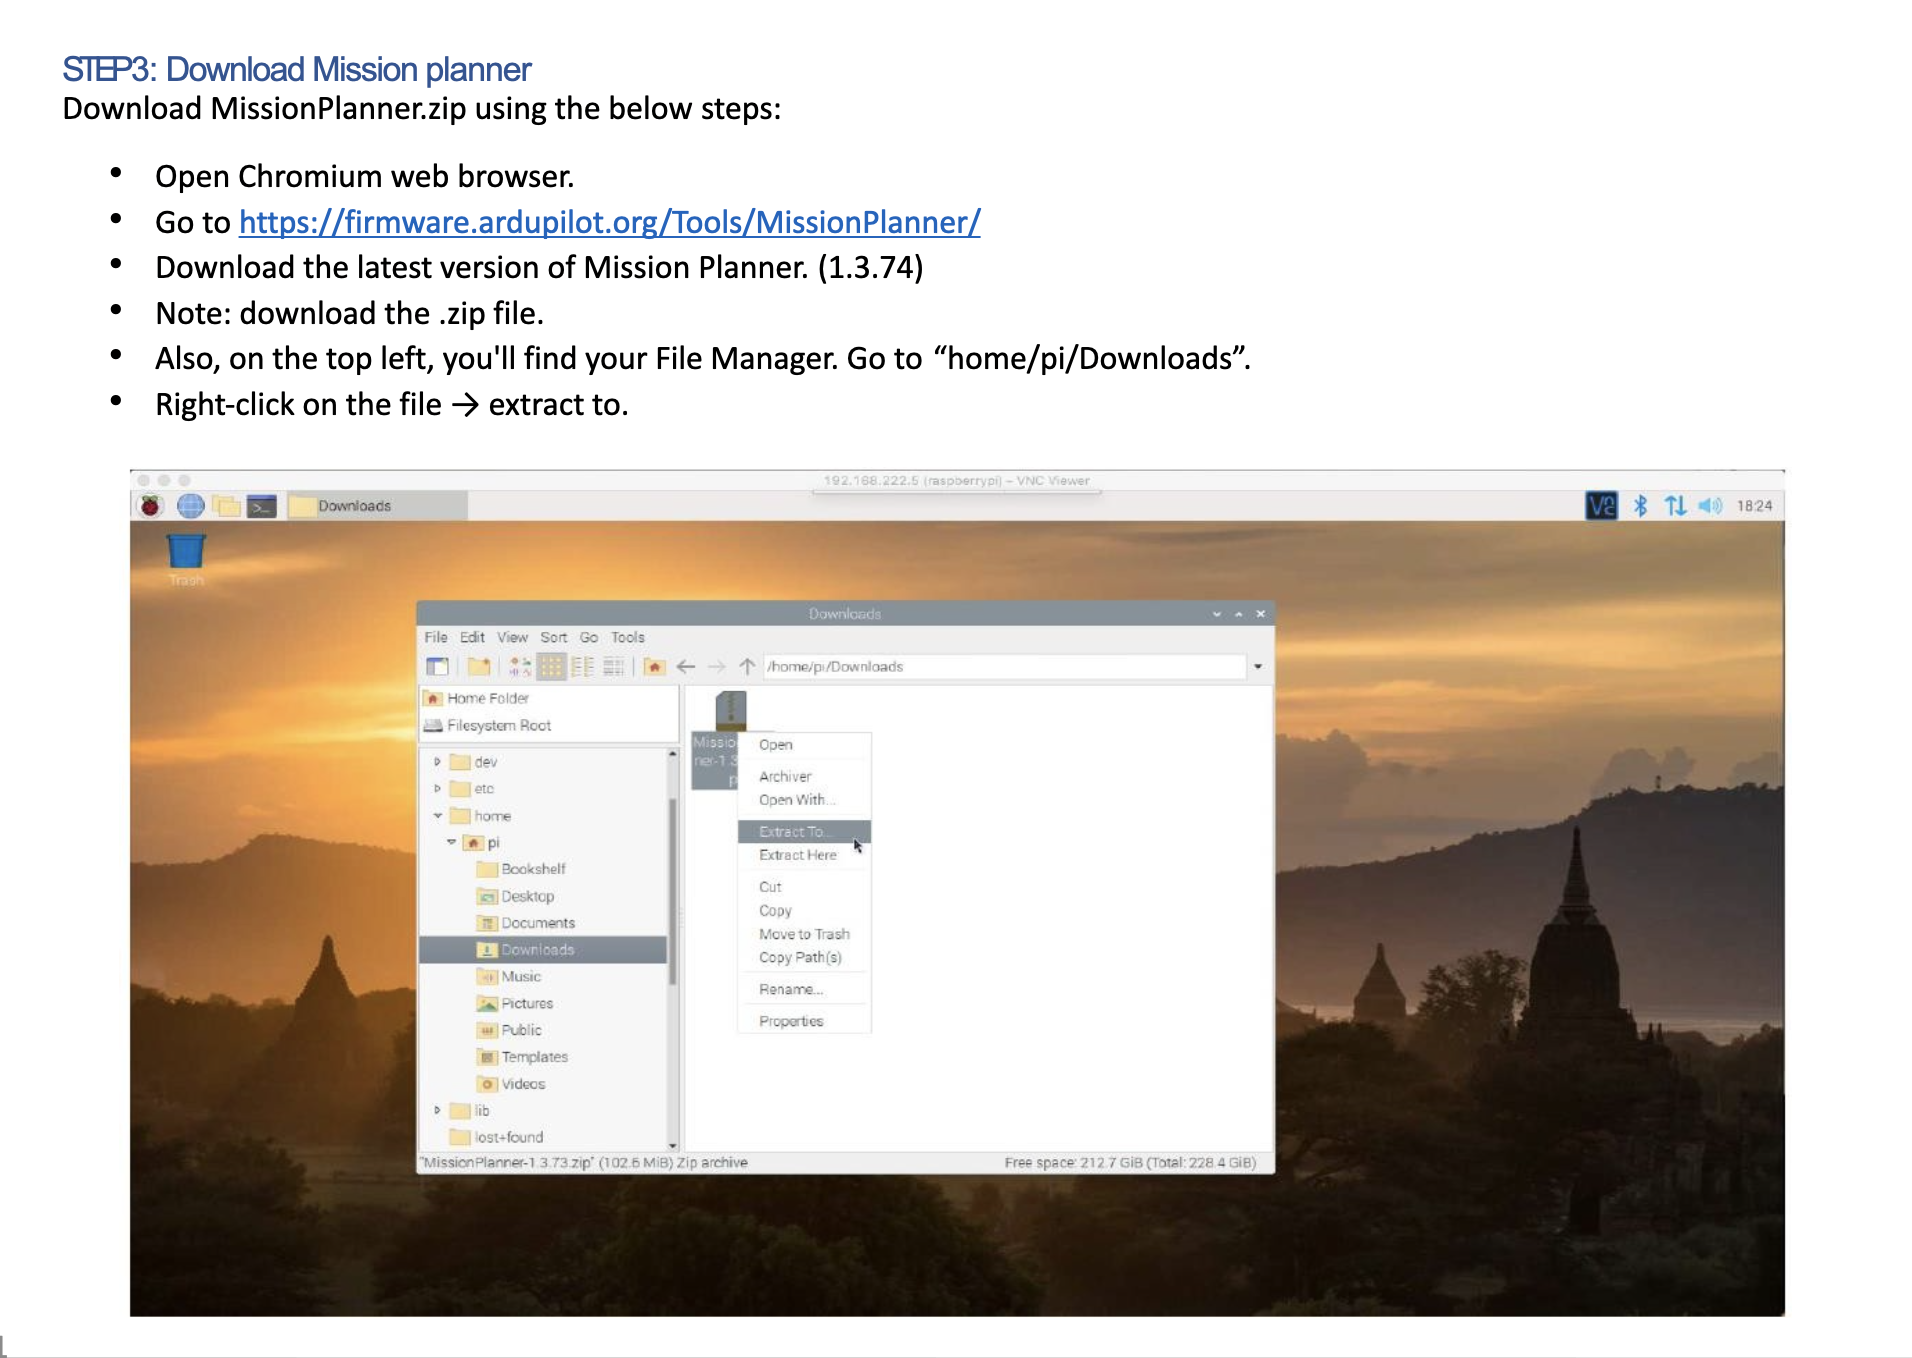
\includegraphics[width=\columnwidth]{./Figures/config_img12.png}
\end{figure}

\begin{figure}[h!]
\centering
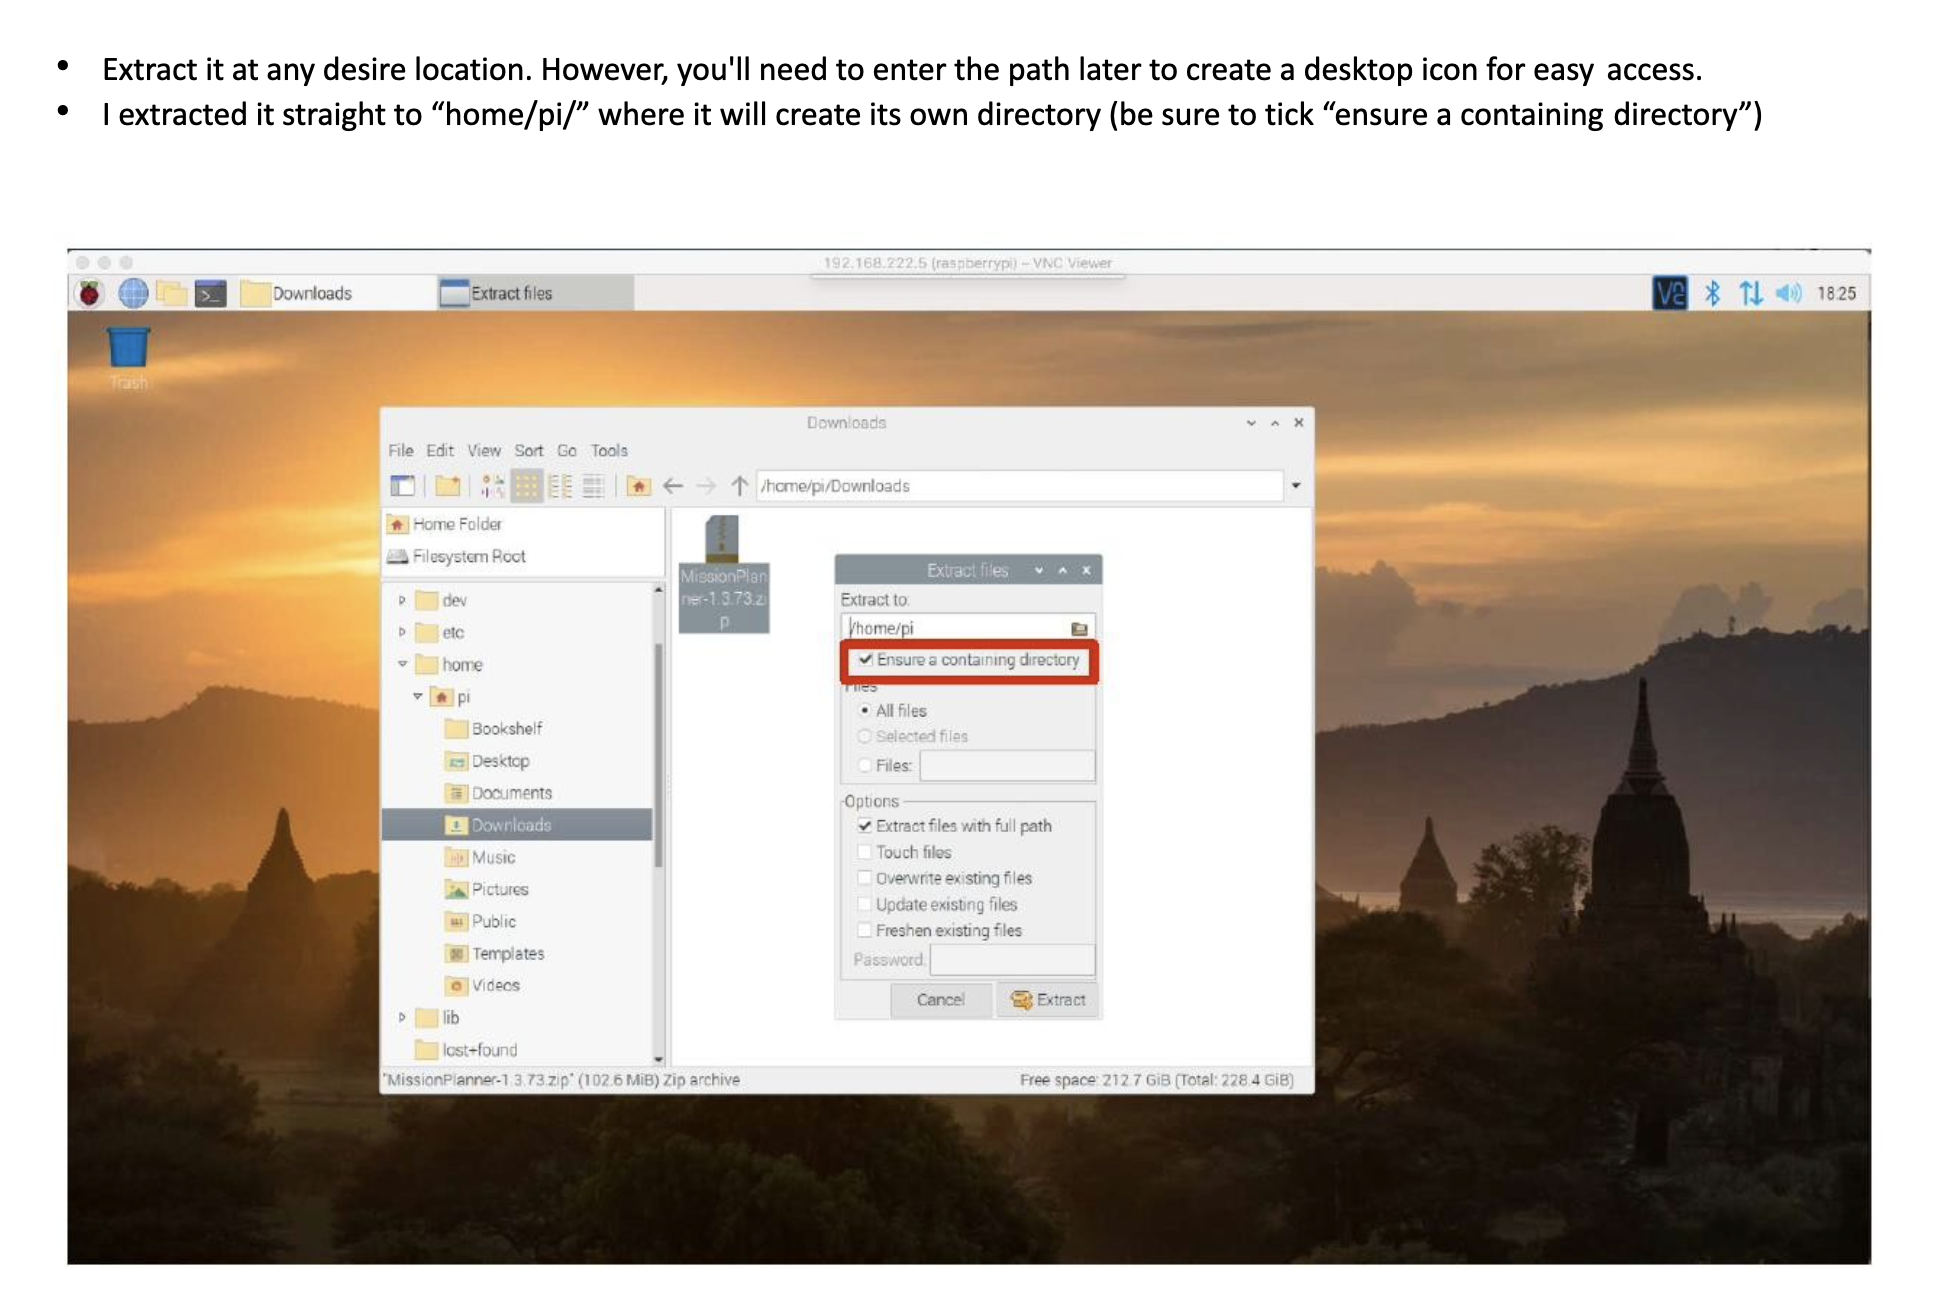
\includegraphics[width=\columnwidth]{./Figures/config_img13.png}
\end{figure}

\begin{figure}[h!]
\centering
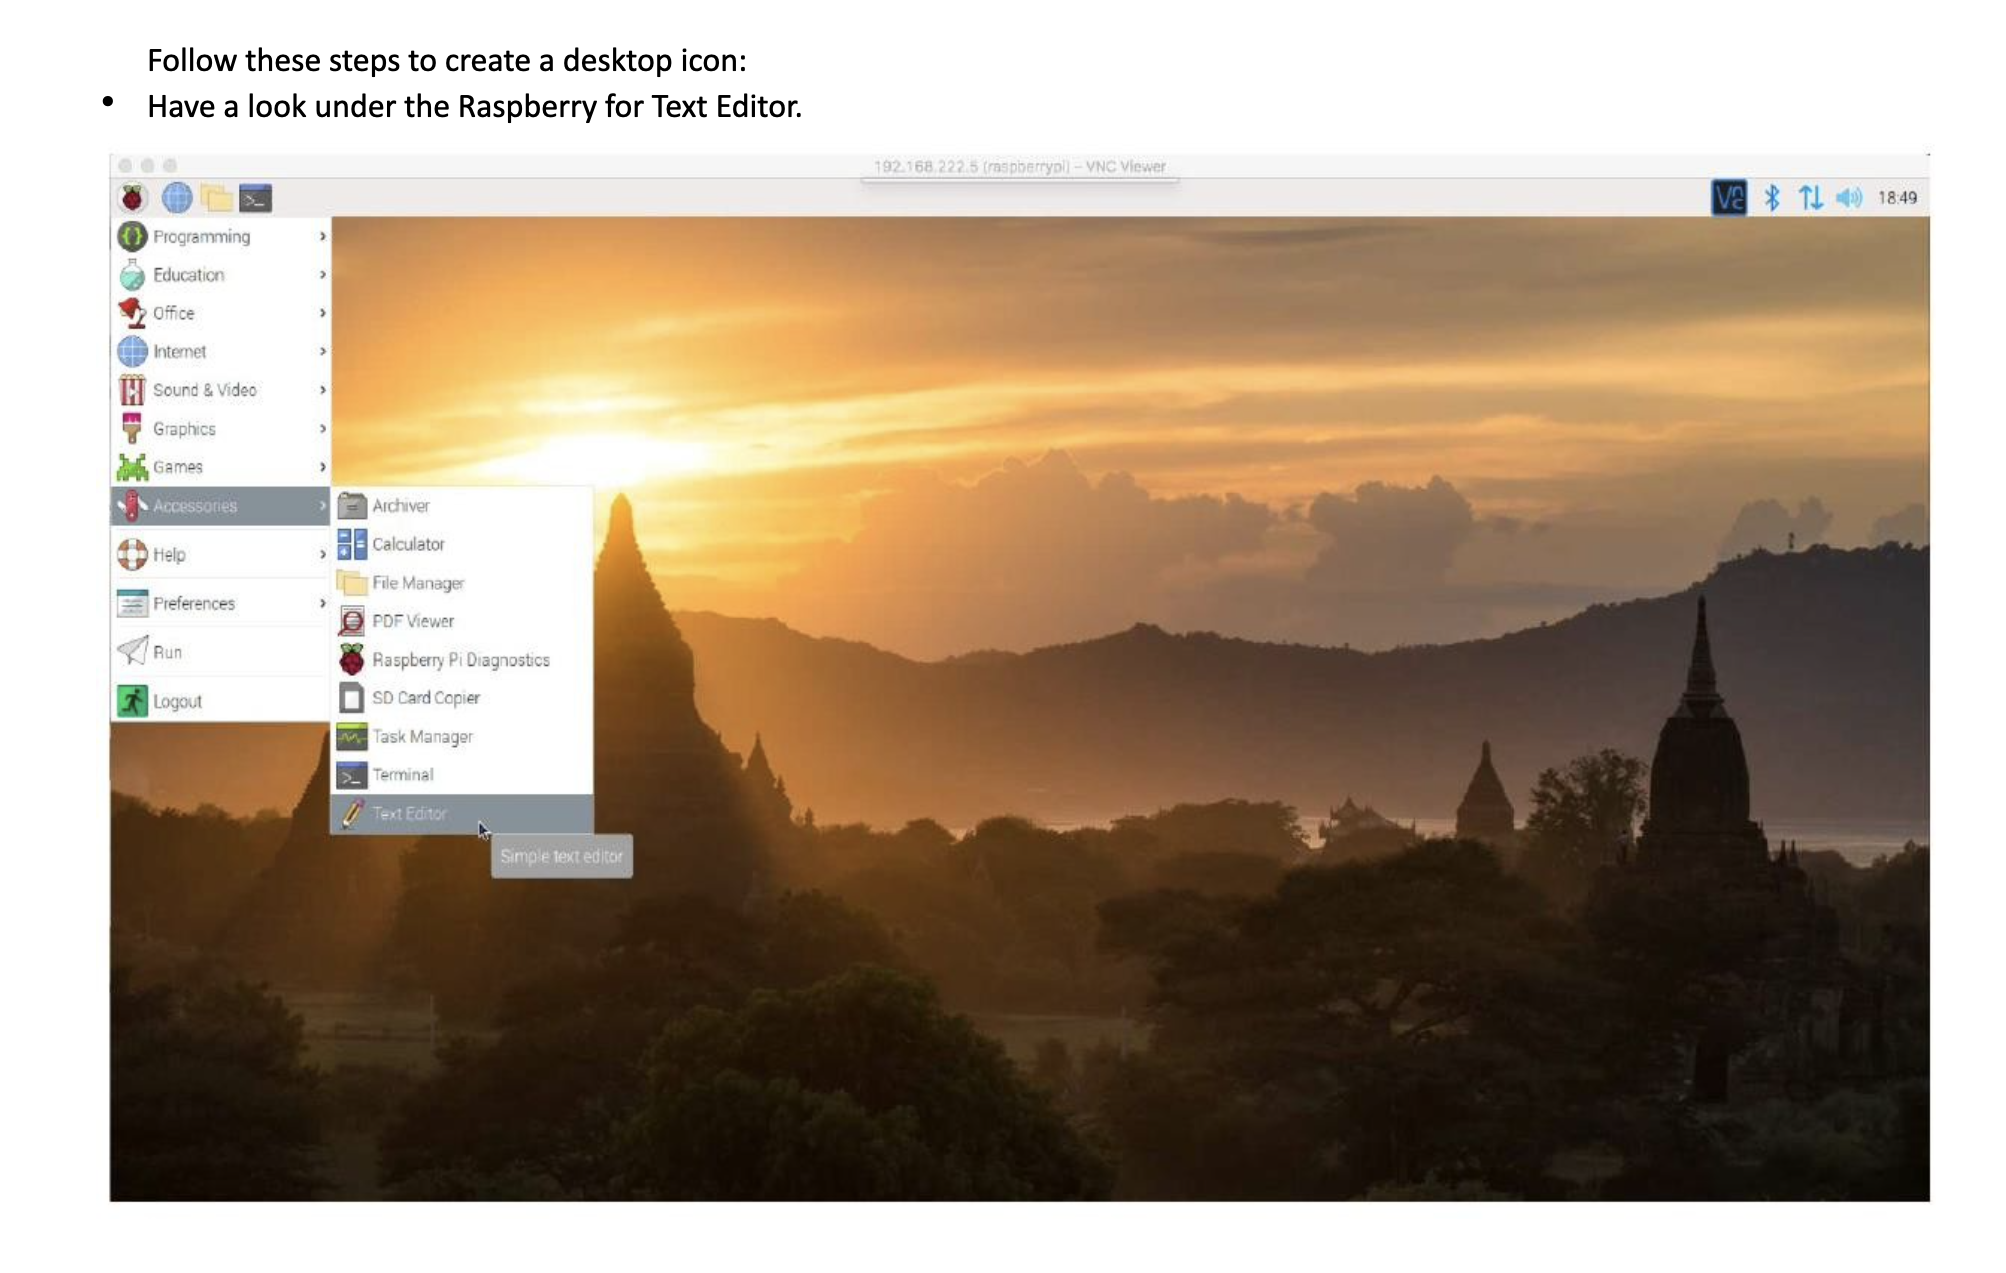
\includegraphics[width=\columnwidth]{./Figures/config_img14.png}
\end{figure}

\begin{figure}[h!]
\centering
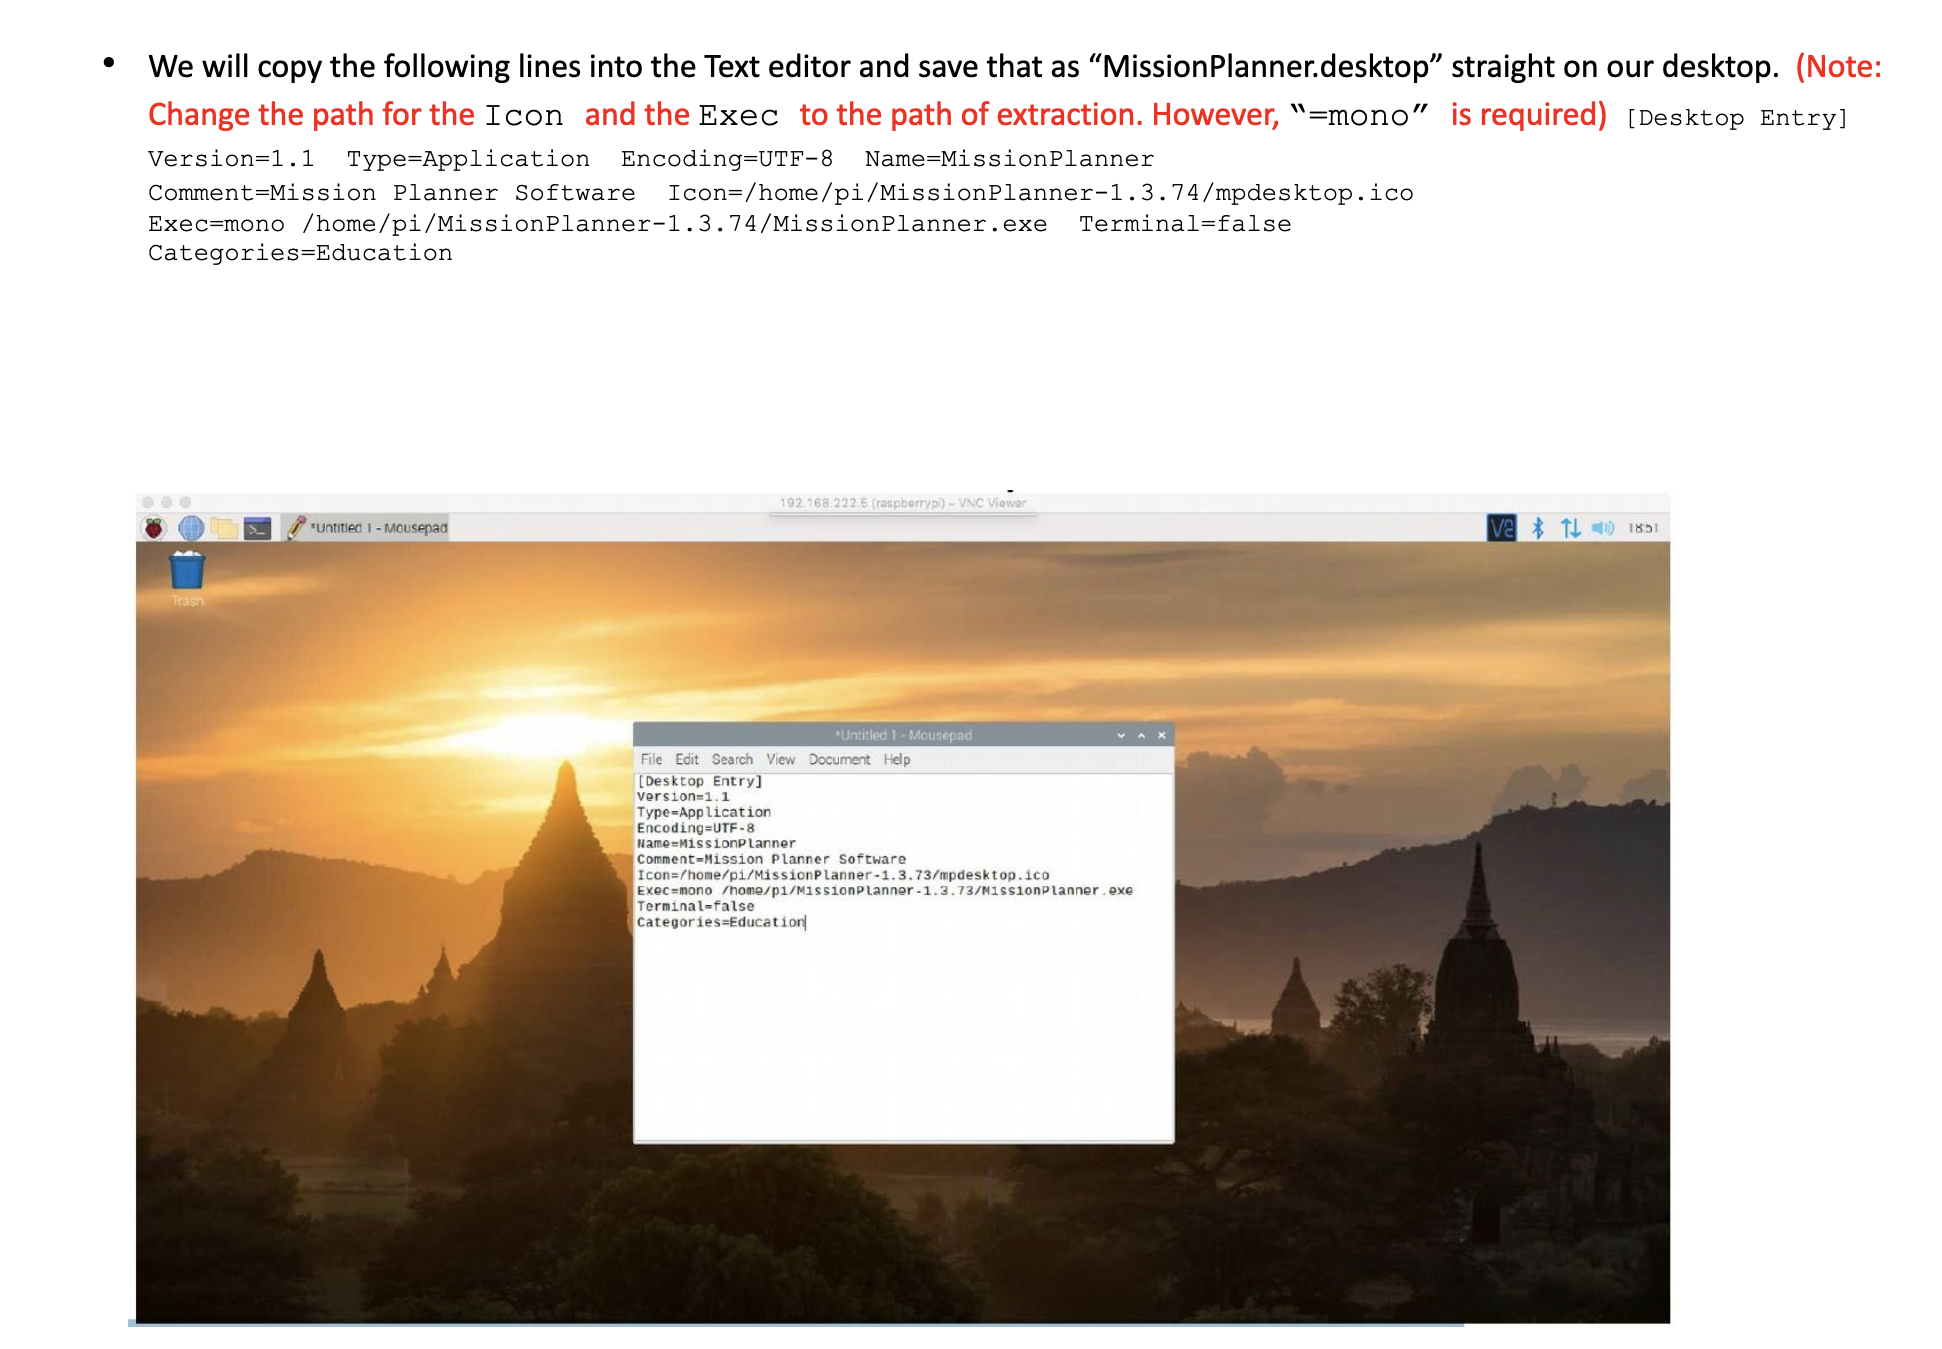
\includegraphics[width=\columnwidth]{./Figures/config_img15.png}
\end{figure}

\begin{figure}[h!]
\centering
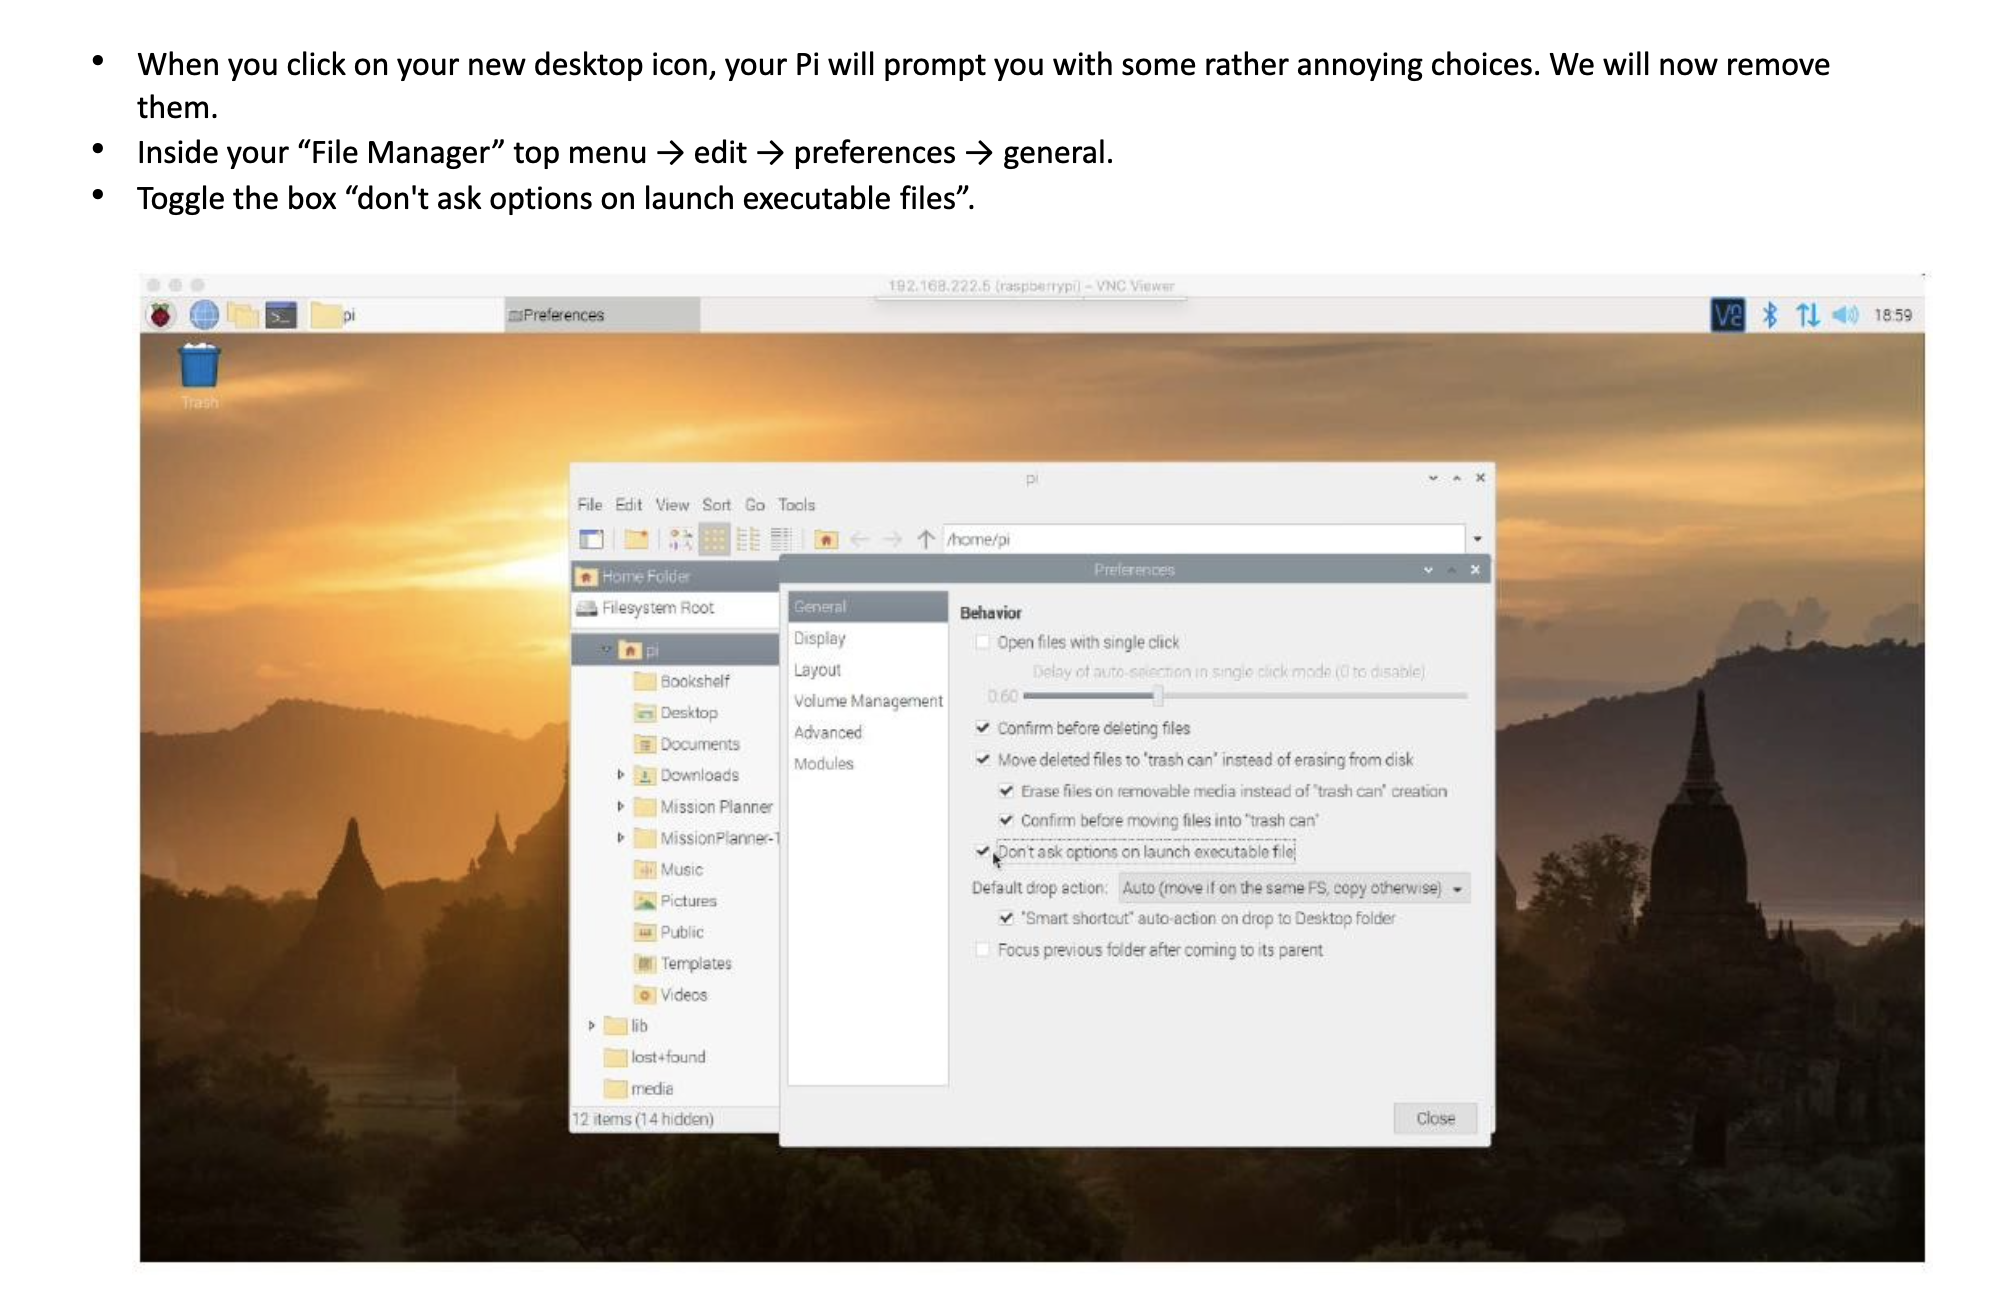
\includegraphics[width=\columnwidth]{./Figures/config_img16.png}
\end{figure}

\begin{figure}[h!]
\centering
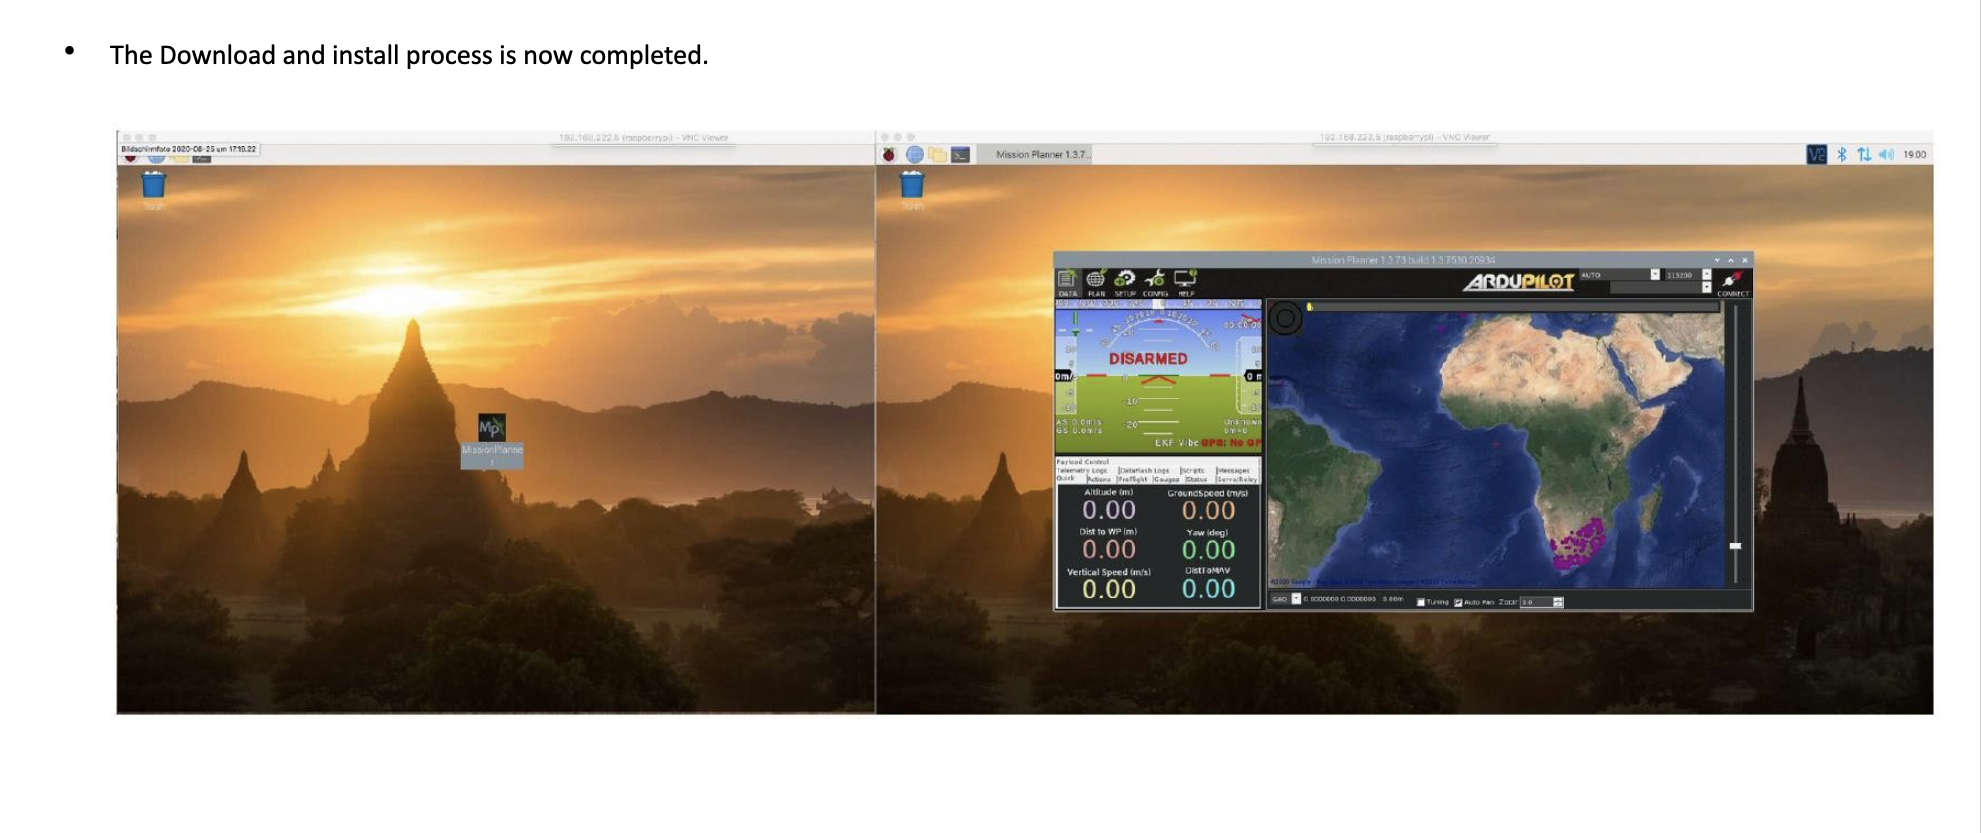
\includegraphics[width=\columnwidth]{./Figures/config_img17.png}
\end{figure}

\begin{figure}[h!]
\centering
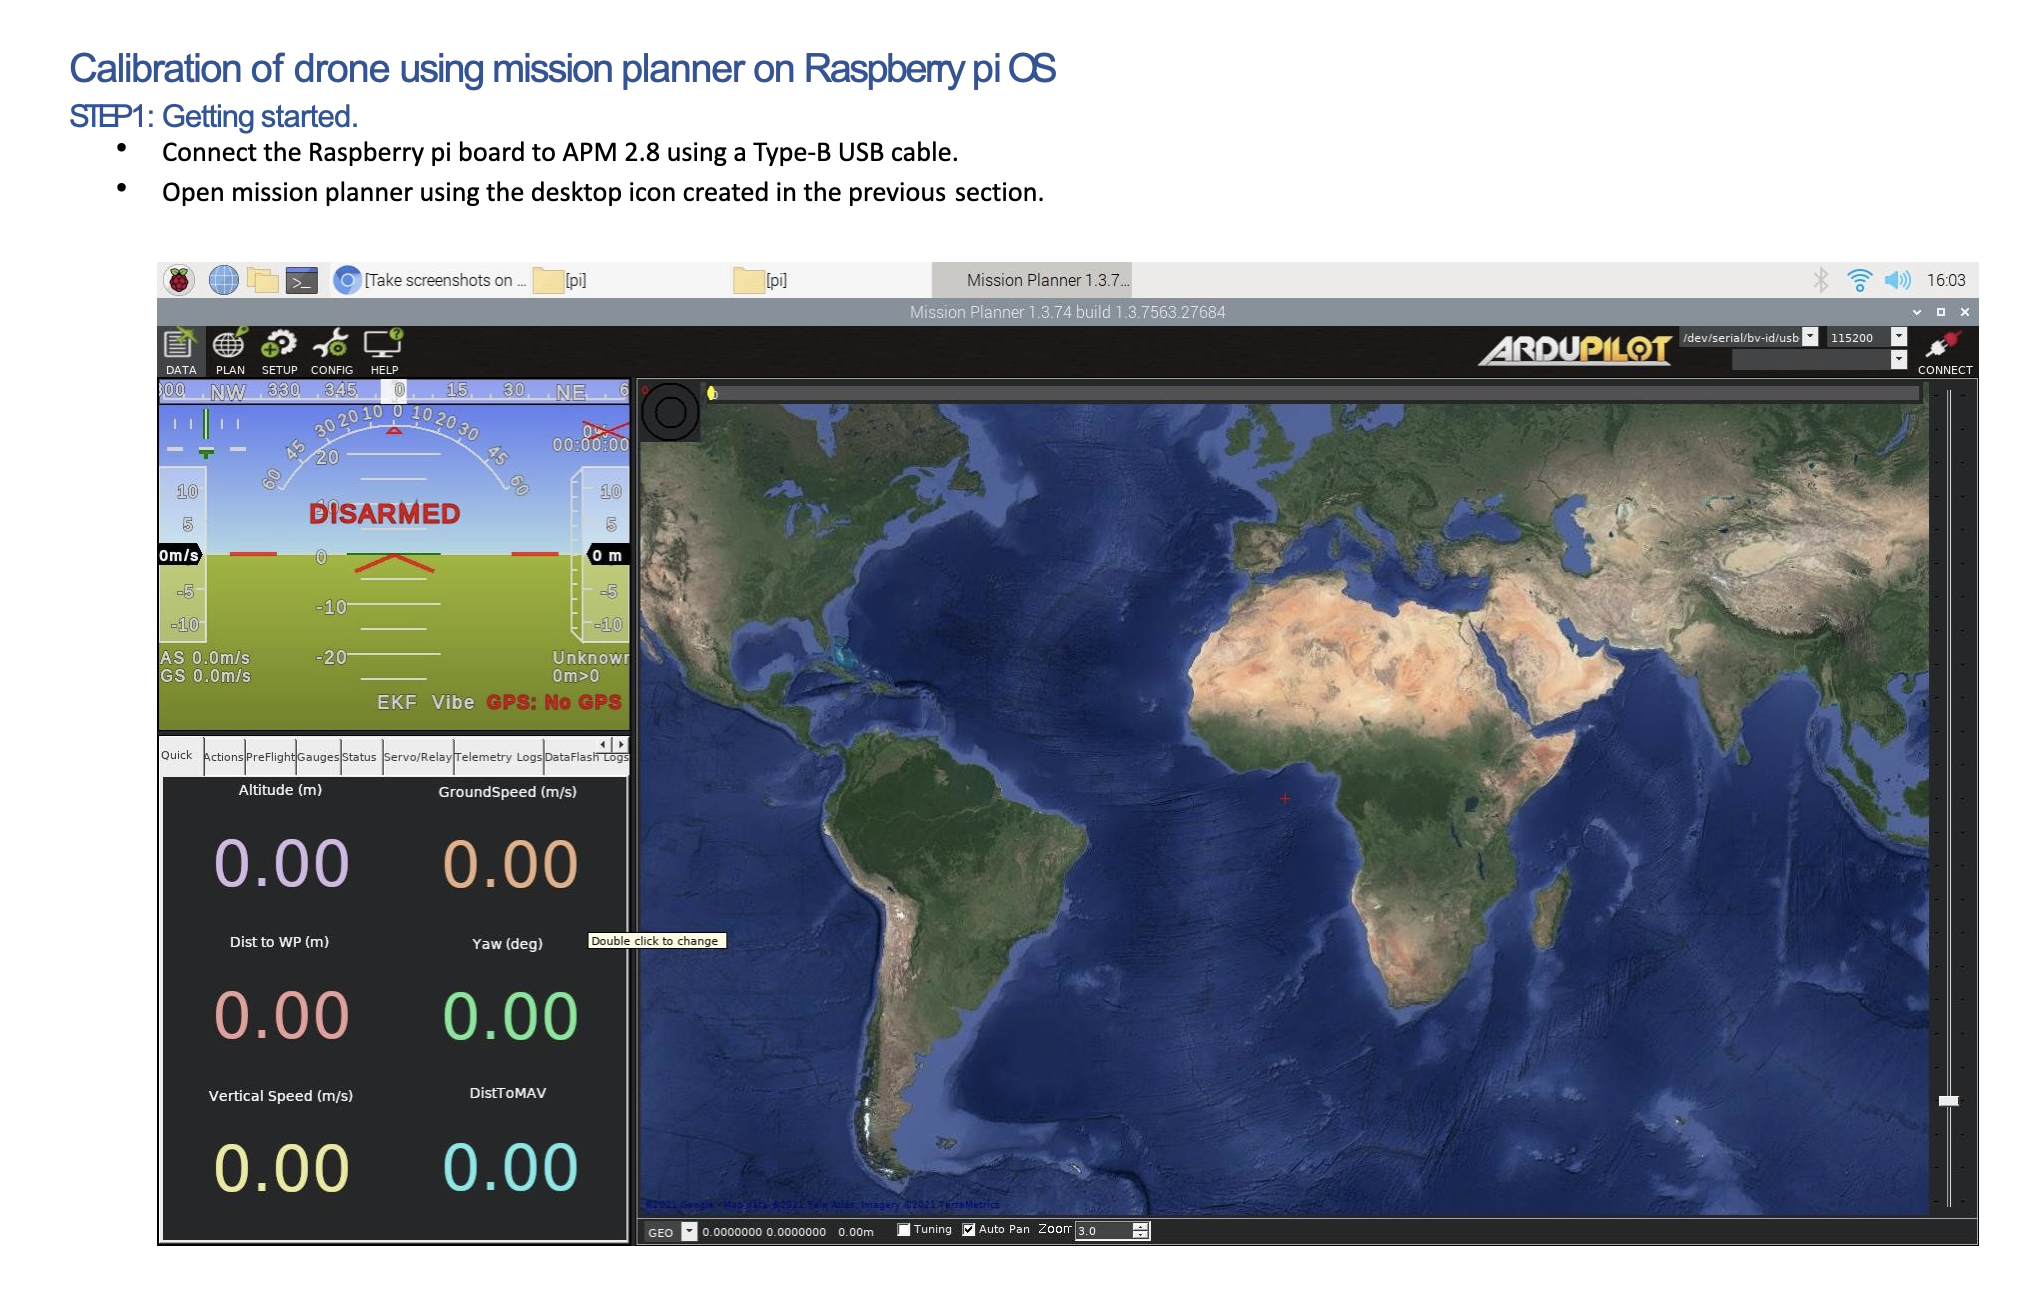
\includegraphics[width=\columnwidth]{./Figures/config_img18.png}
\end{figure}

\begin{figure}[h!]
\centering
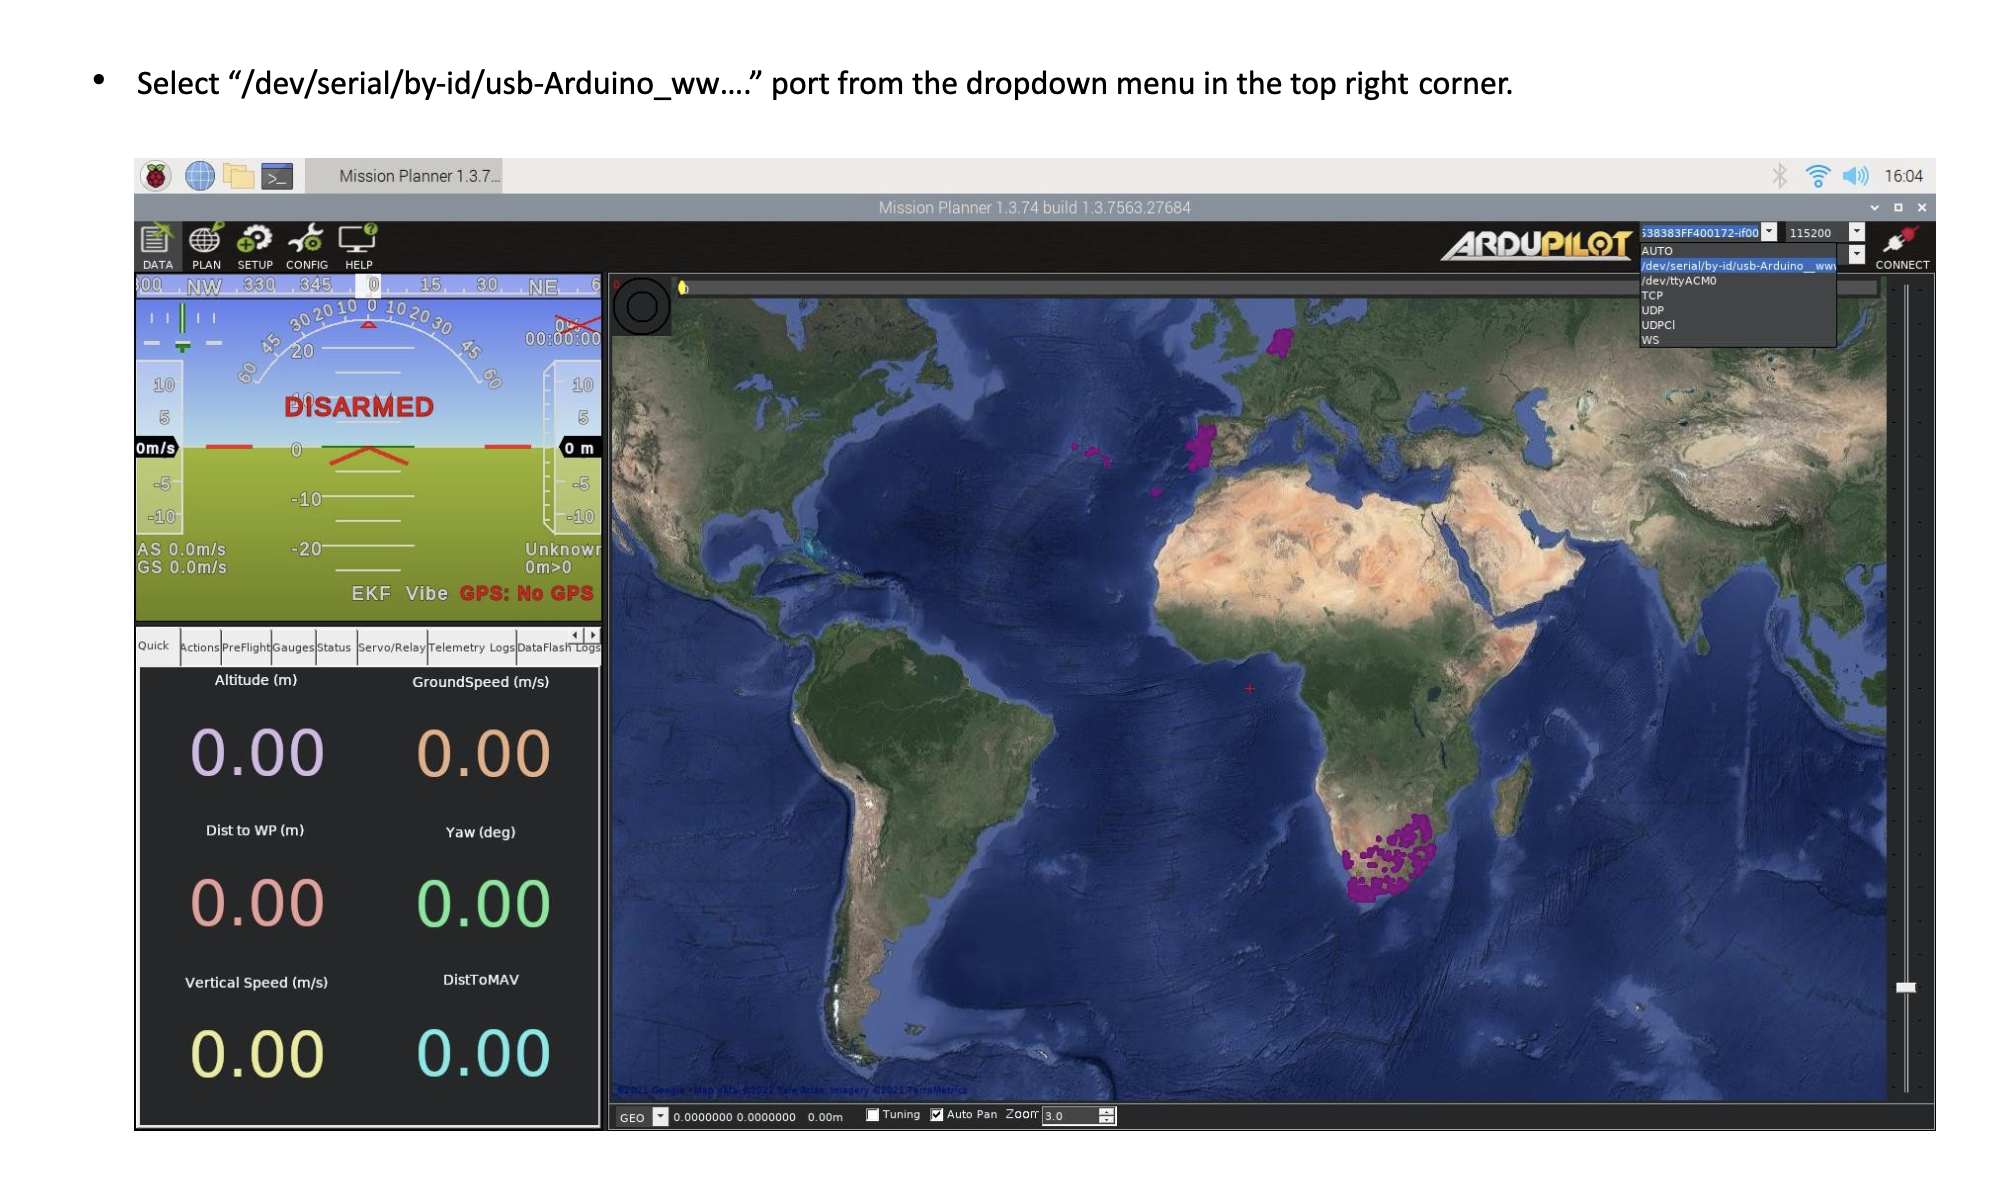
\includegraphics[width=\columnwidth]{./Figures/config_img19.png}
\end{figure}

\begin{figure}[h!]
\centering
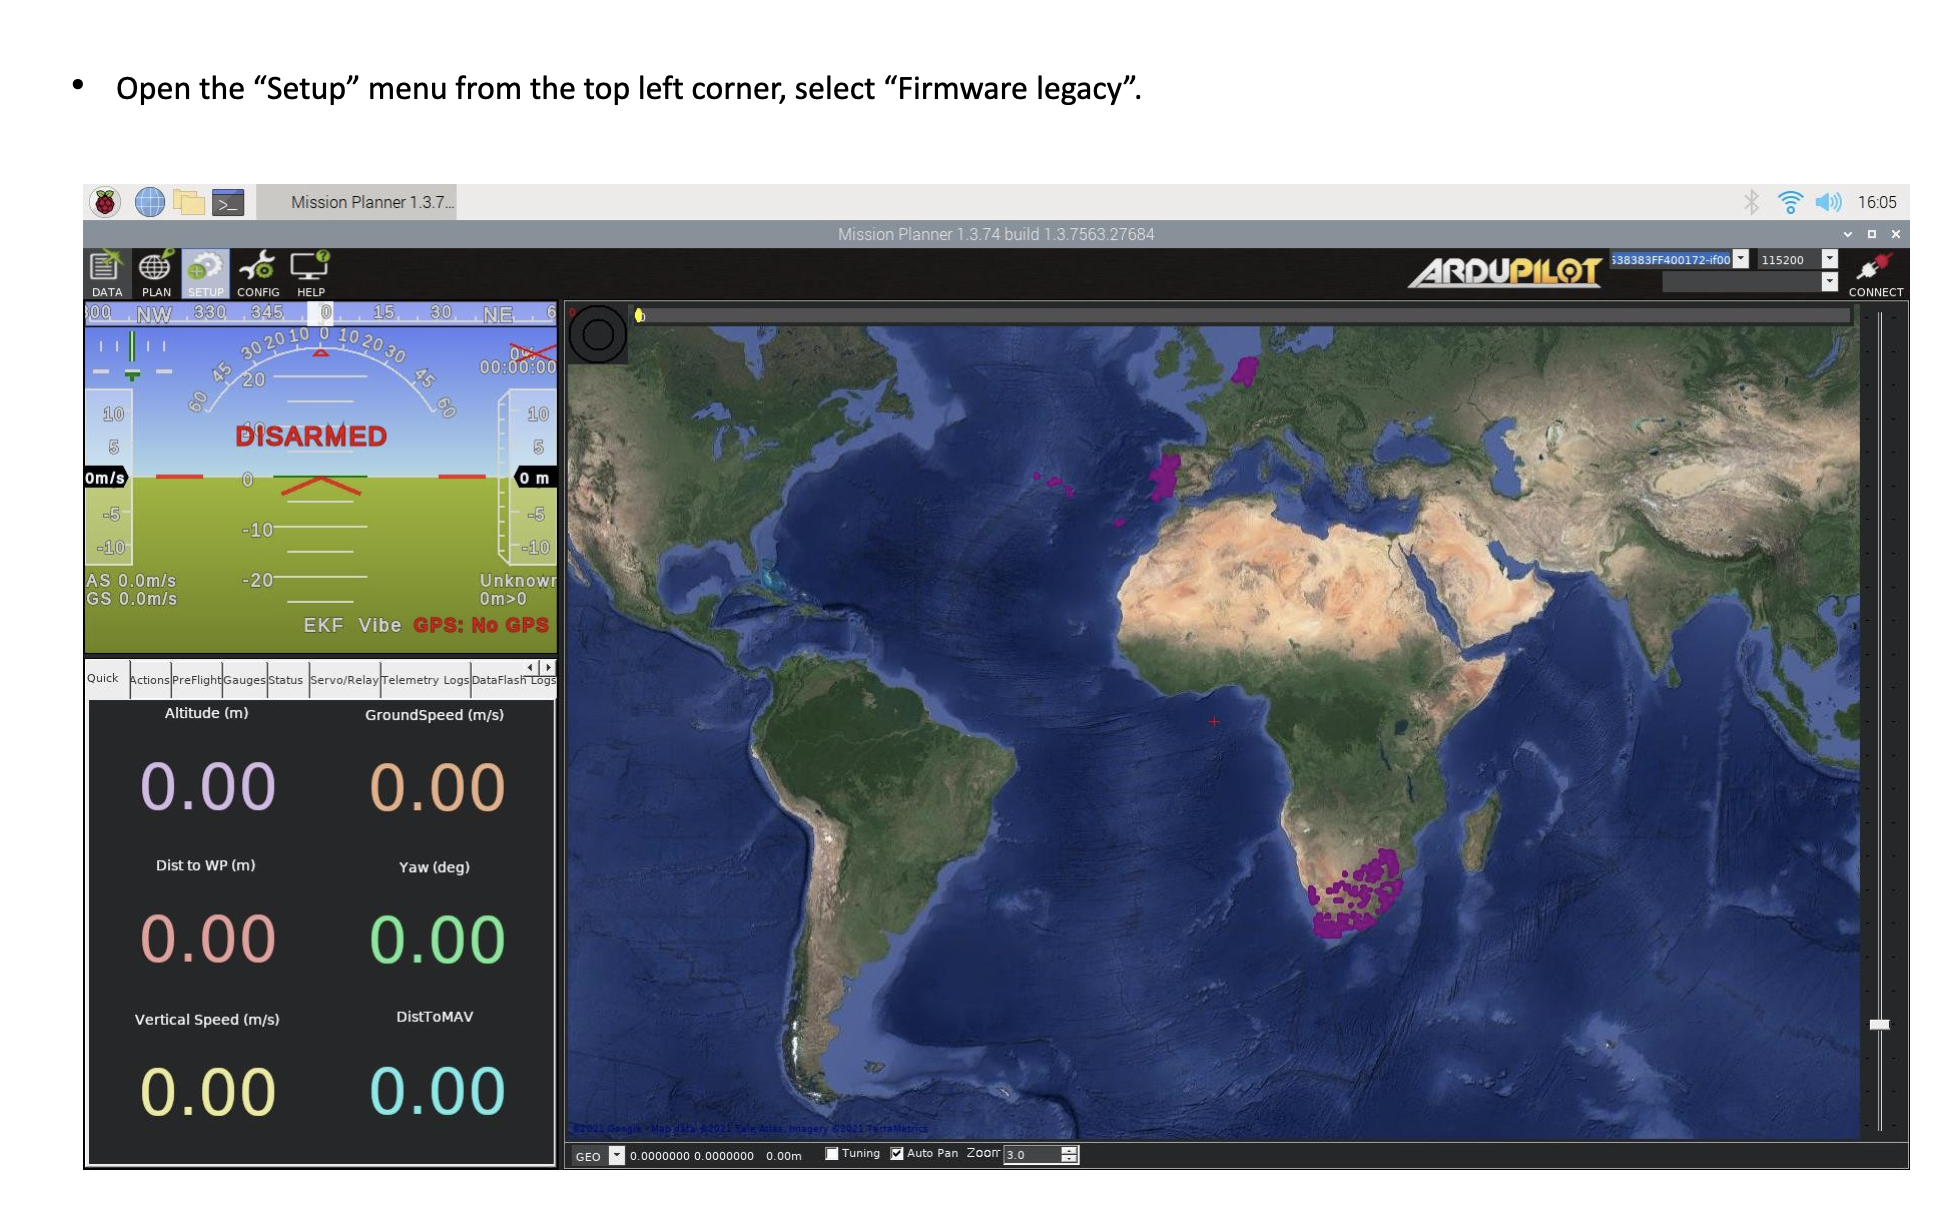
\includegraphics[width=\columnwidth]{./Figures/config_img20.png}
\end{figure}

\begin{figure}[h!]
\centering
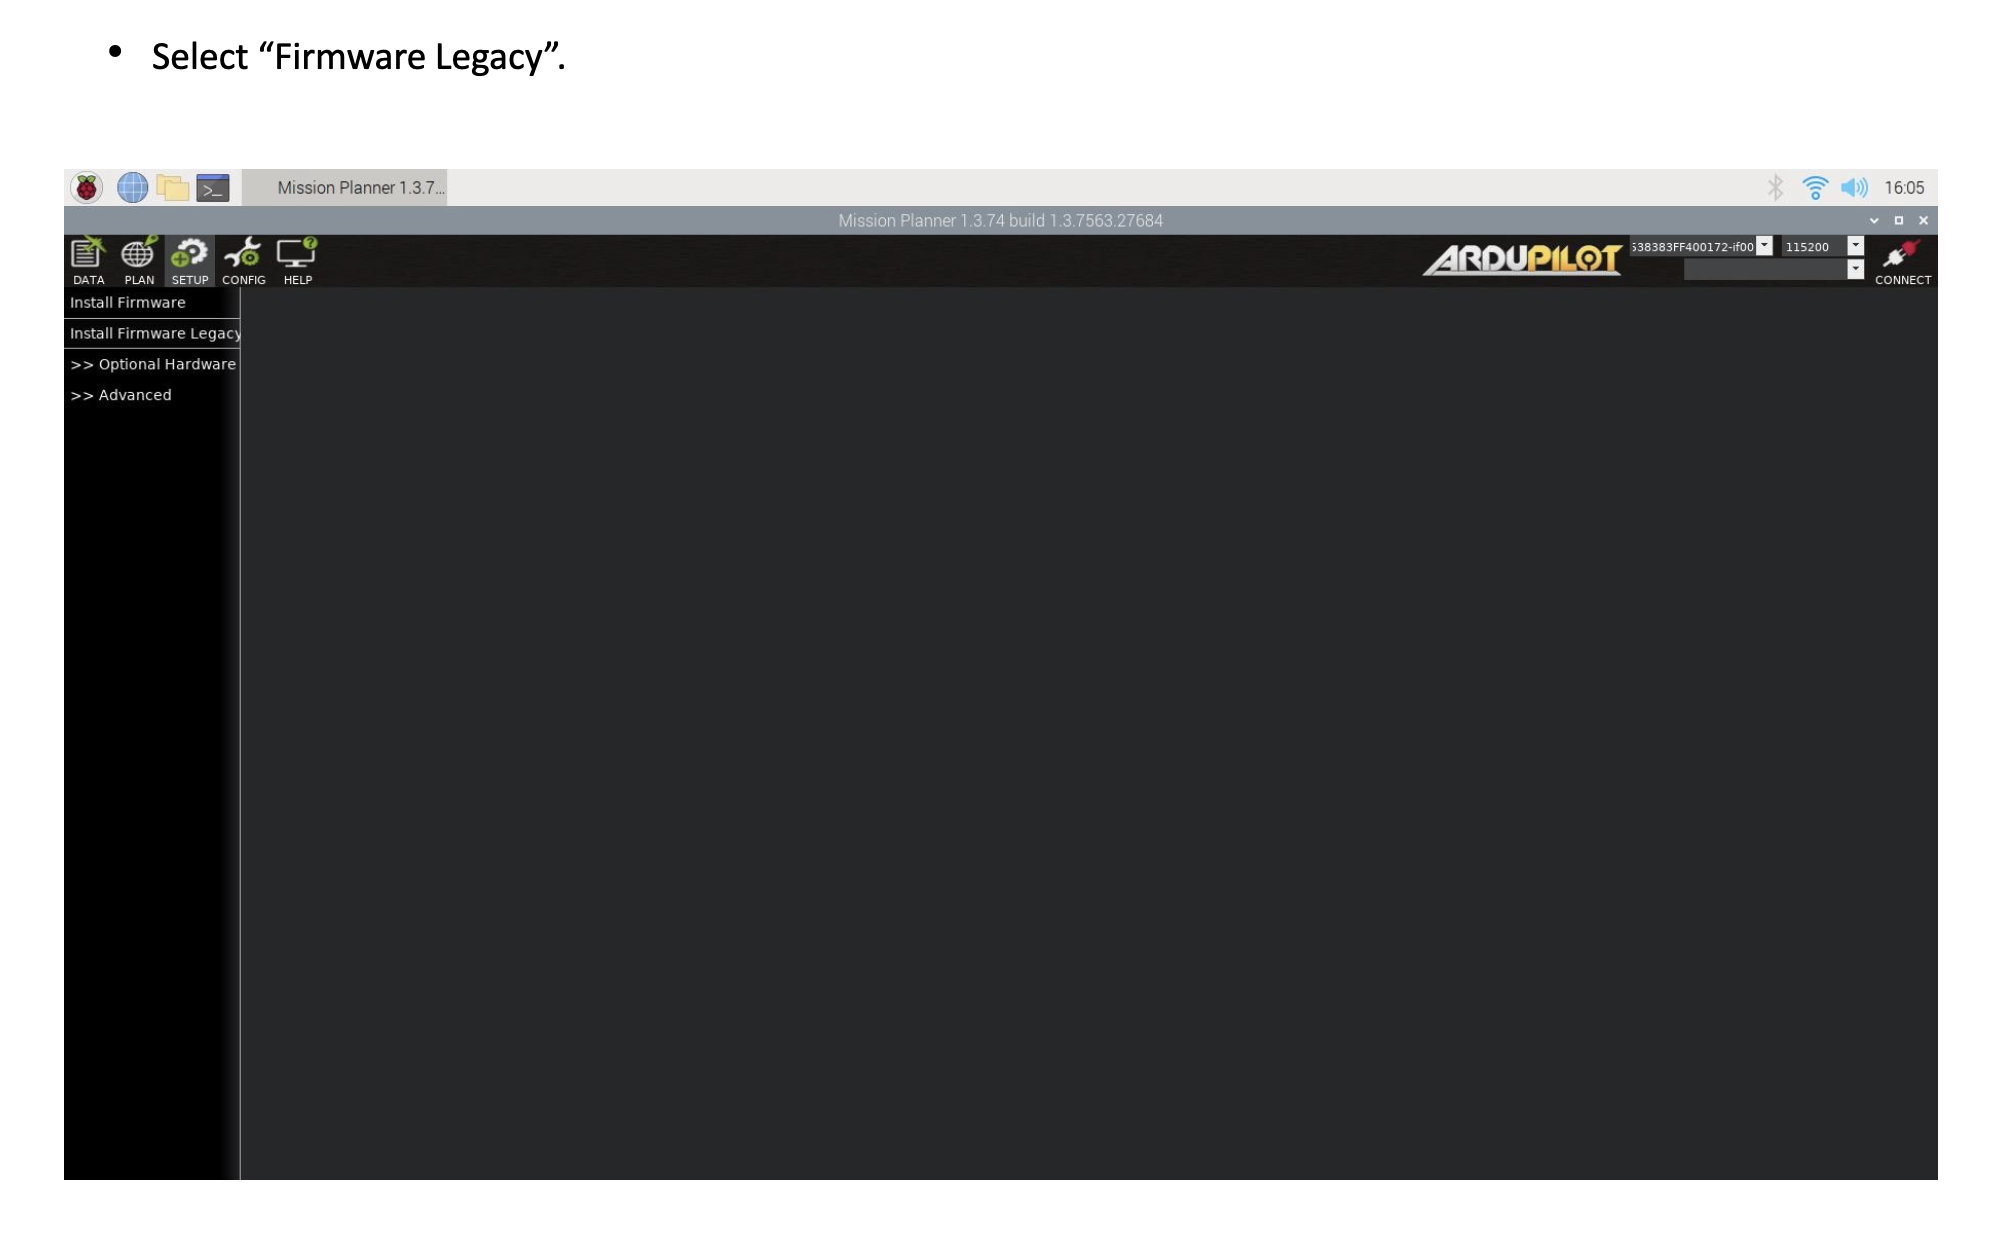
\includegraphics[width=\columnwidth]{./Figures/config_img21.png}
\end{figure}

\begin{figure}[h!]
\centering
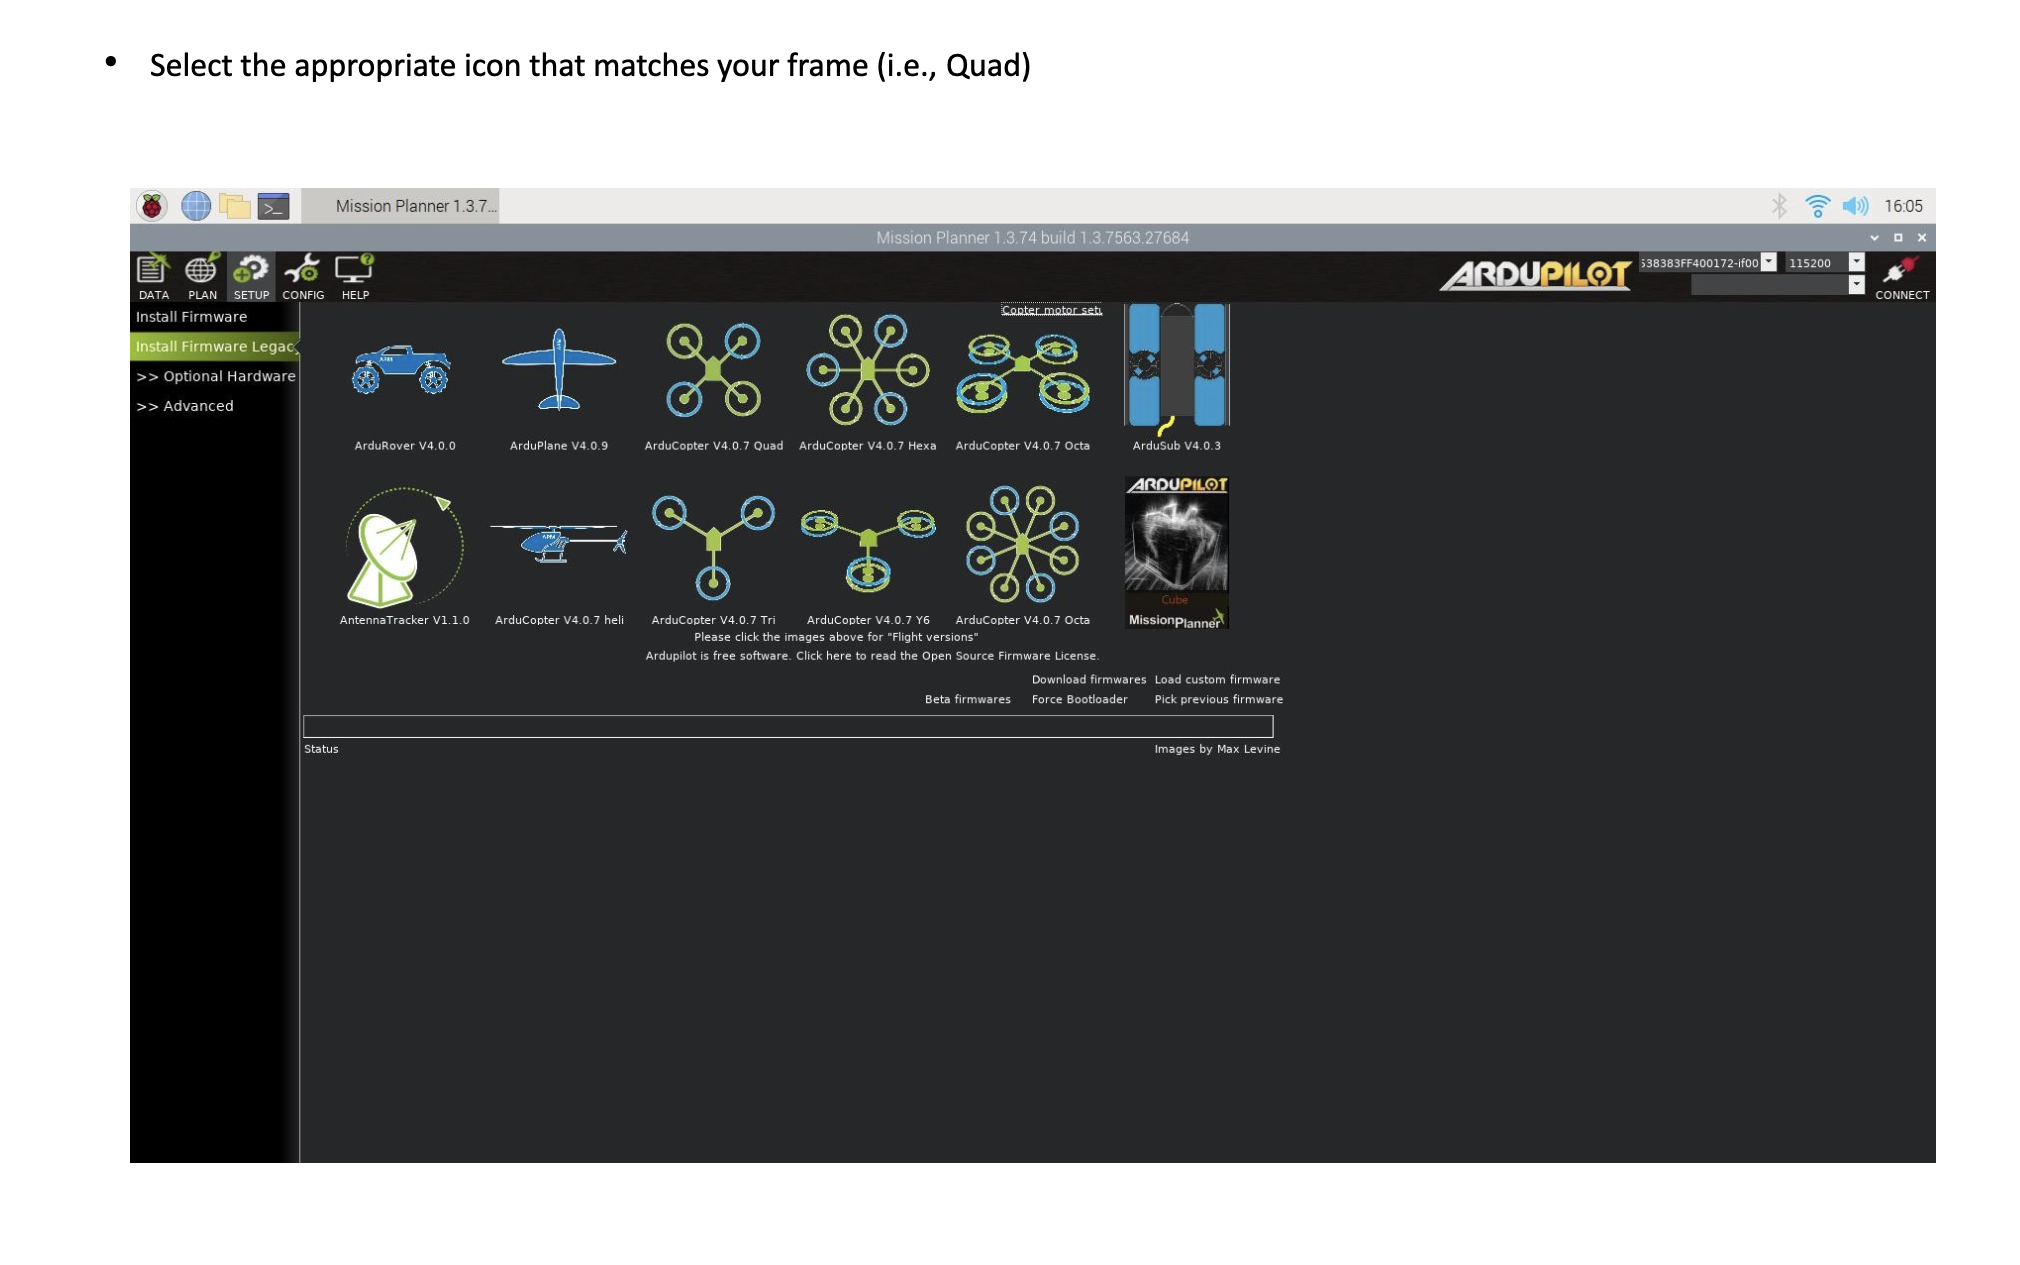
\includegraphics[width=\columnwidth]{./Figures/config_img22.png}
\end{figure}

\begin{figure}[h!]
\centering
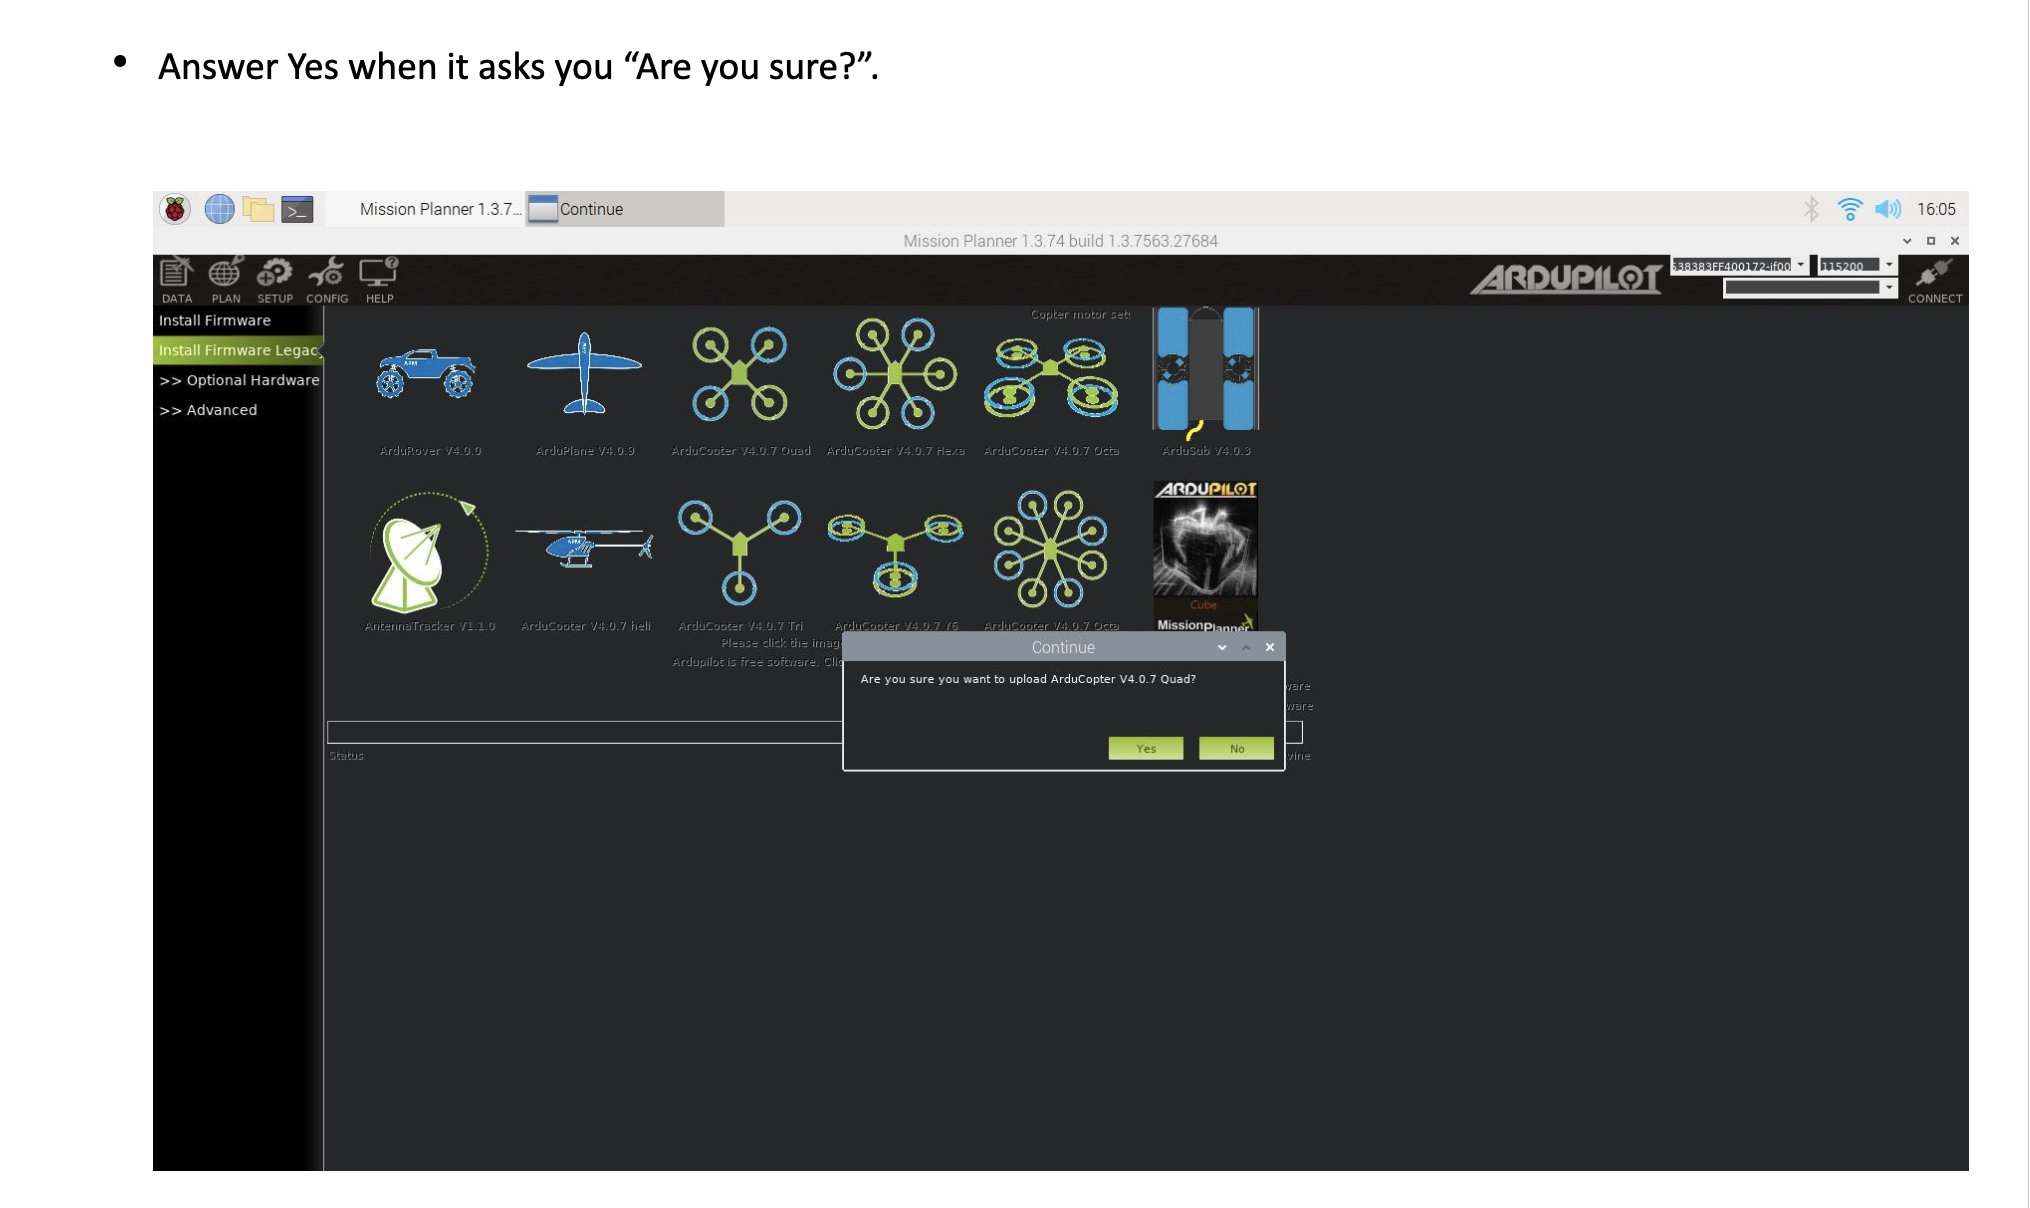
\includegraphics[width=\columnwidth]{./Figures/config_img23.png}
\end{figure}

\begin{figure}[h!]
\centering
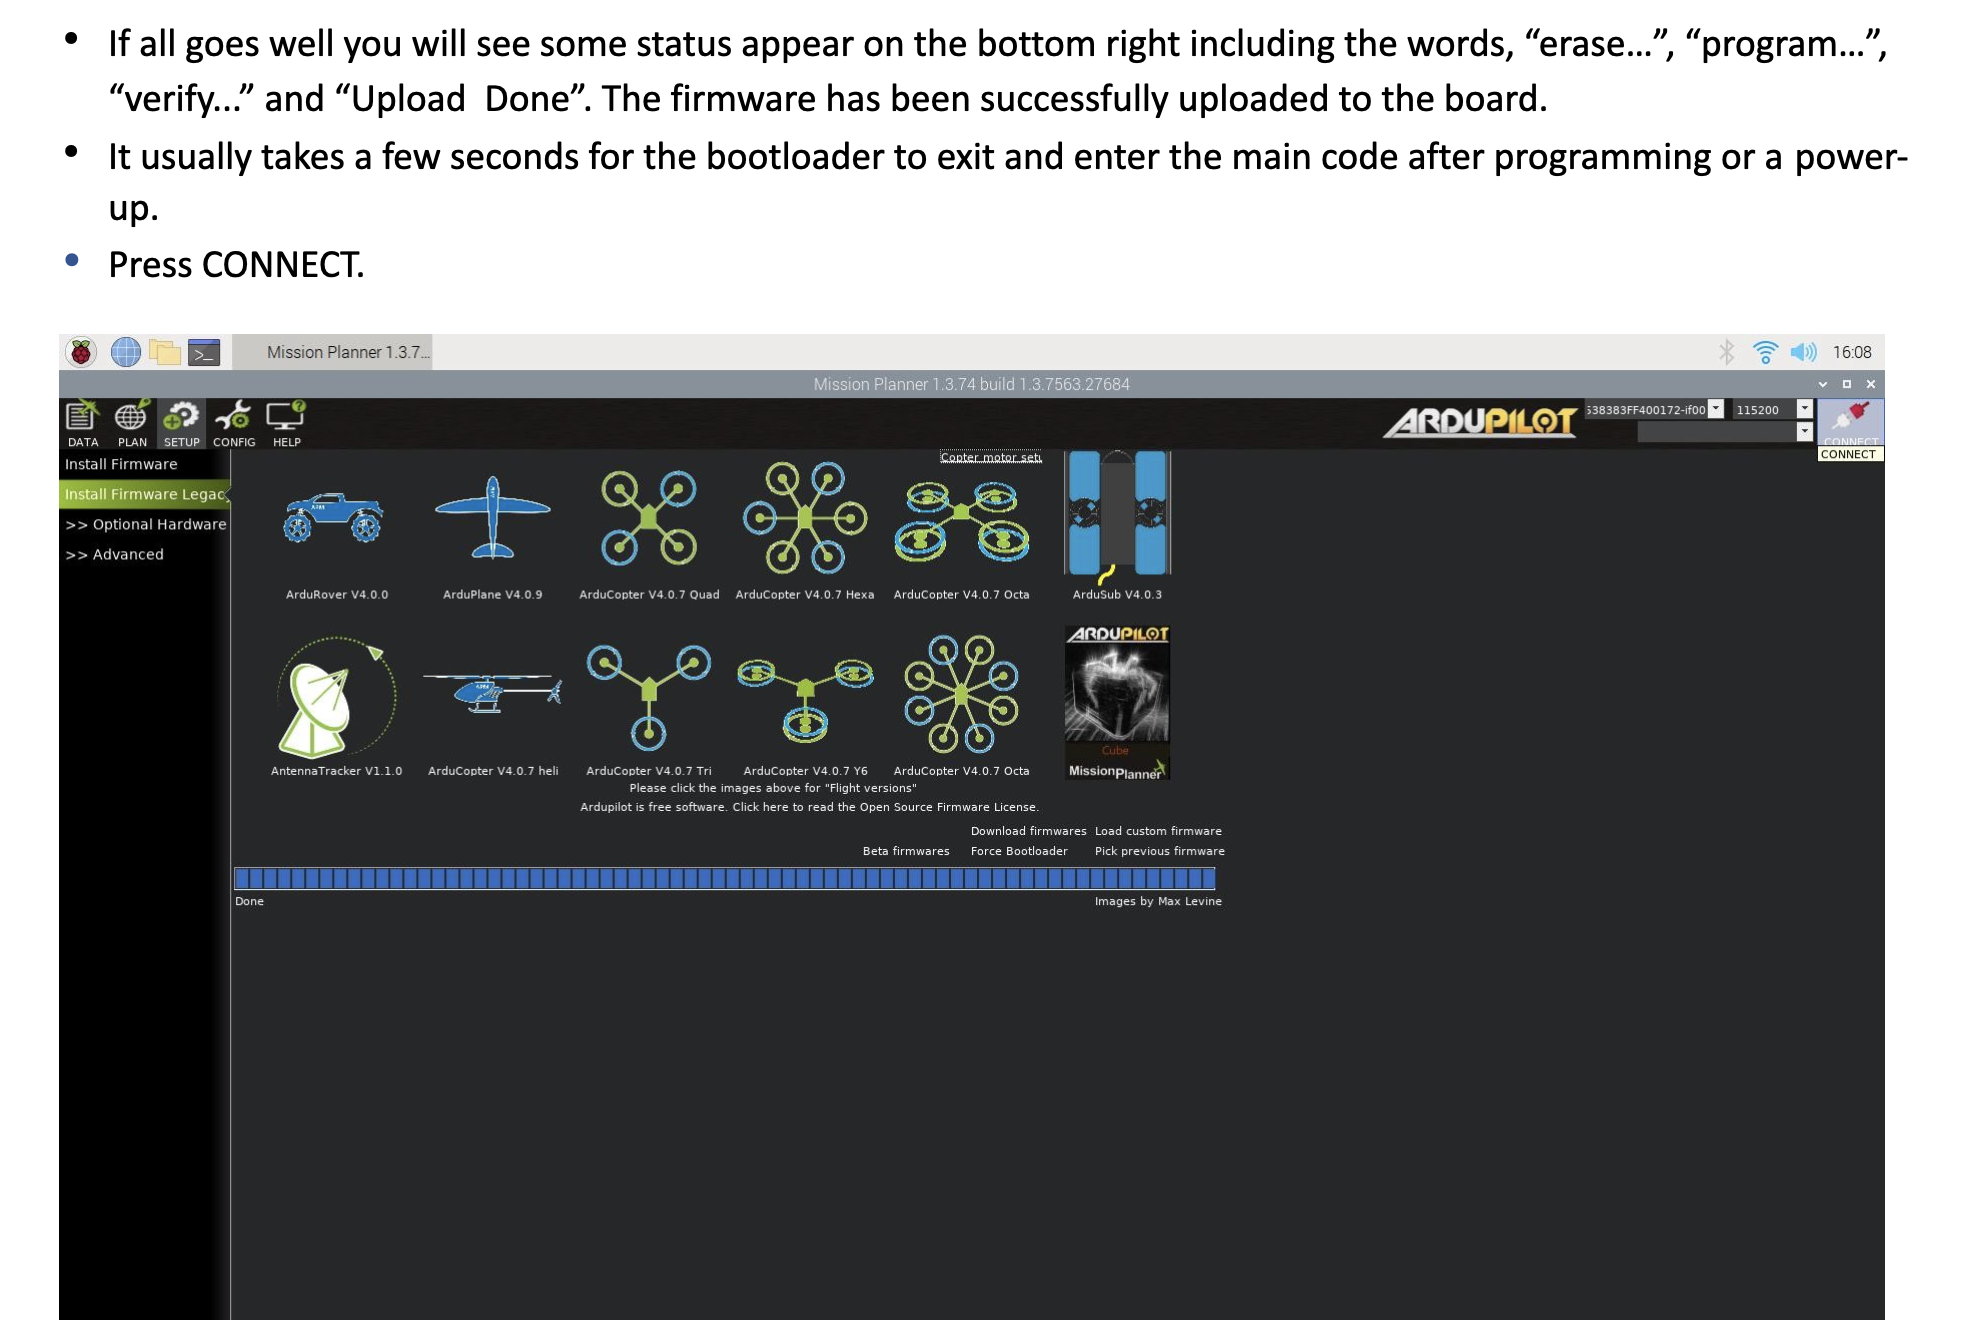
\includegraphics[width=\columnwidth]{./Figures/config_img24.png}
\end{figure}

\begin{figure}[h!]
\centering
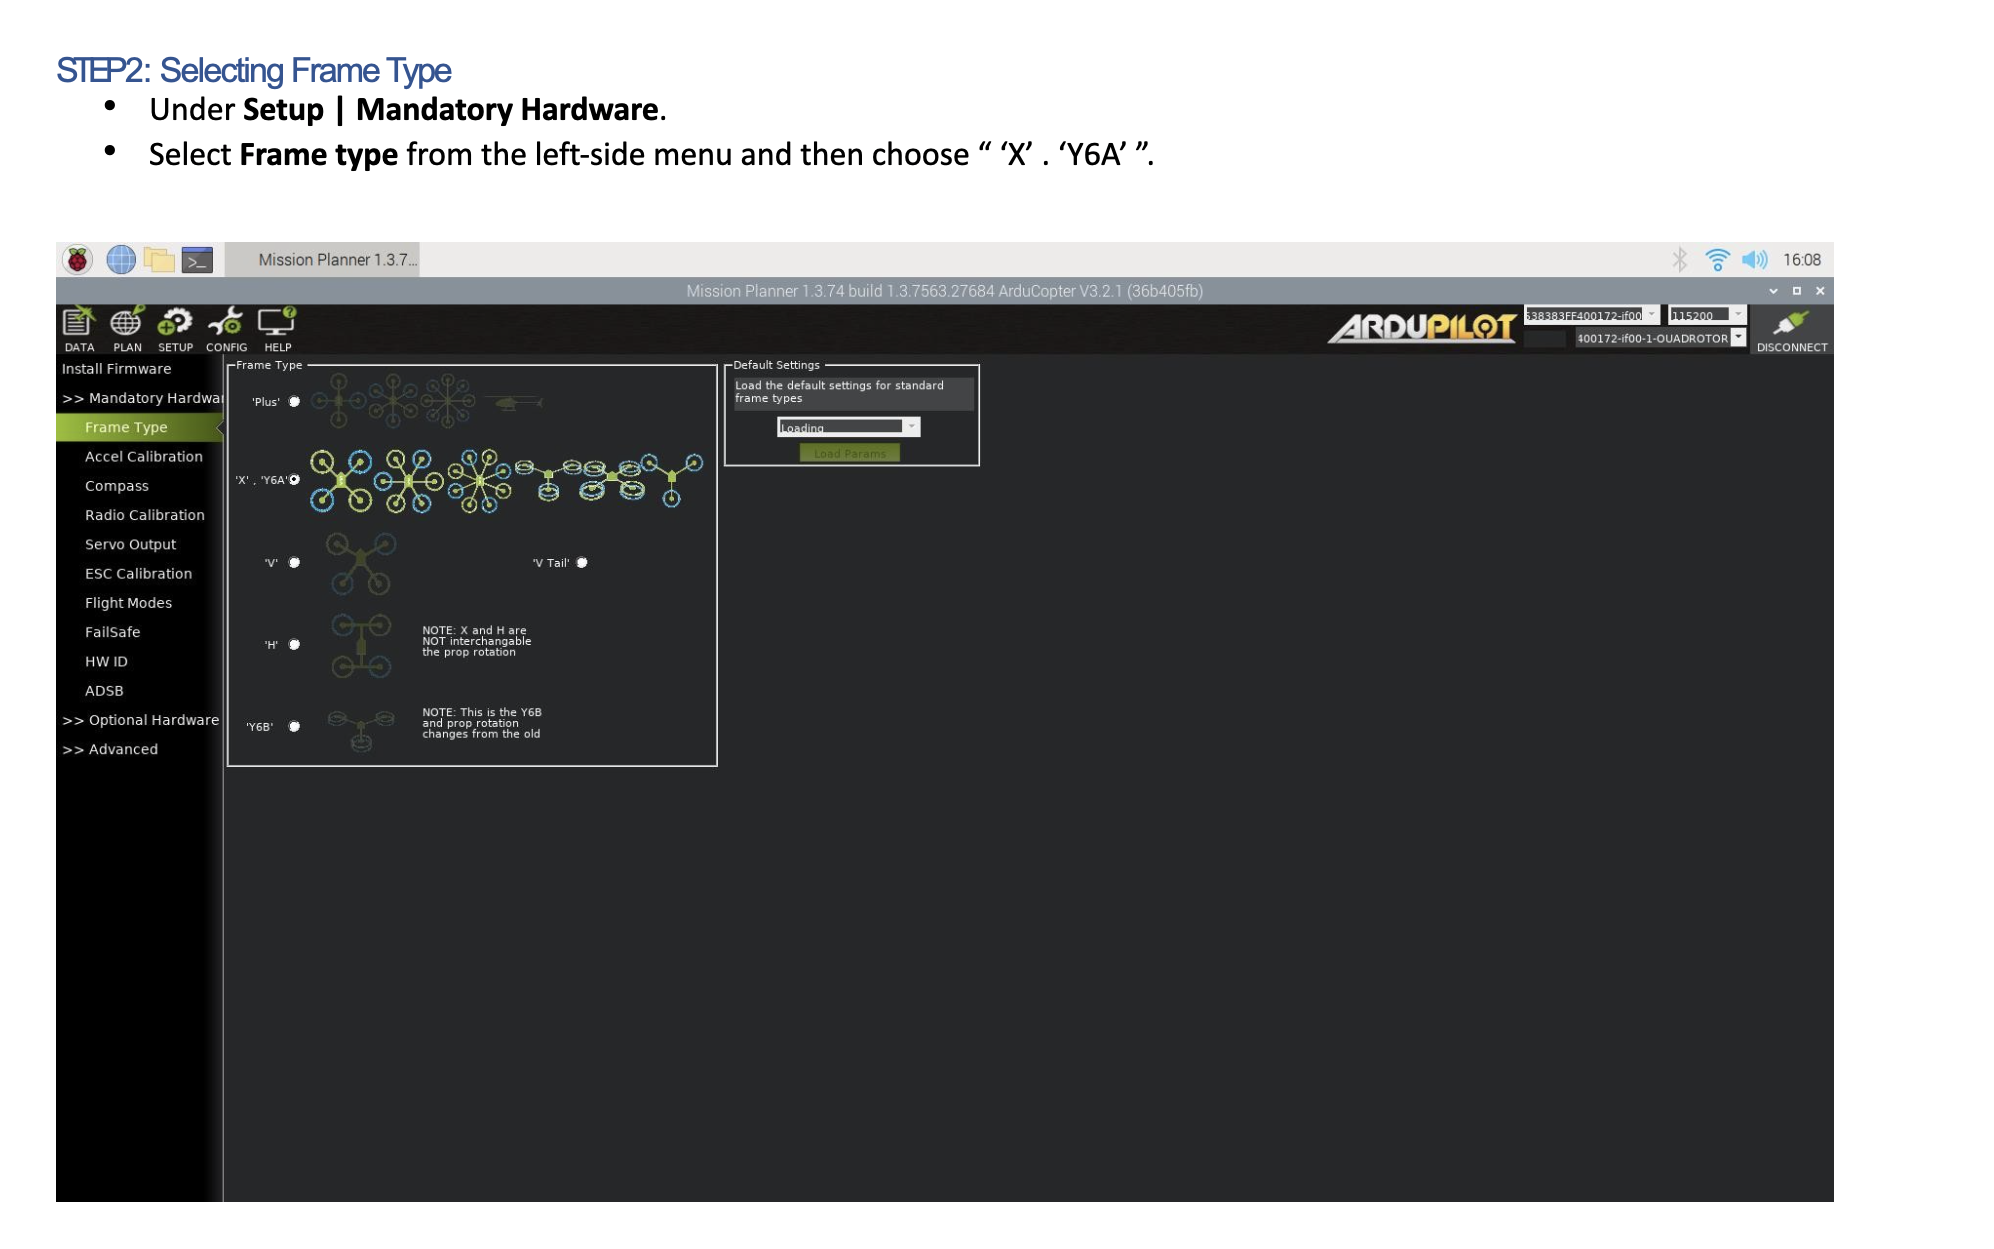
\includegraphics[width=\columnwidth]{./Figures/config_img25.png}
\end{figure}

\begin{figure}[h!]
\centering
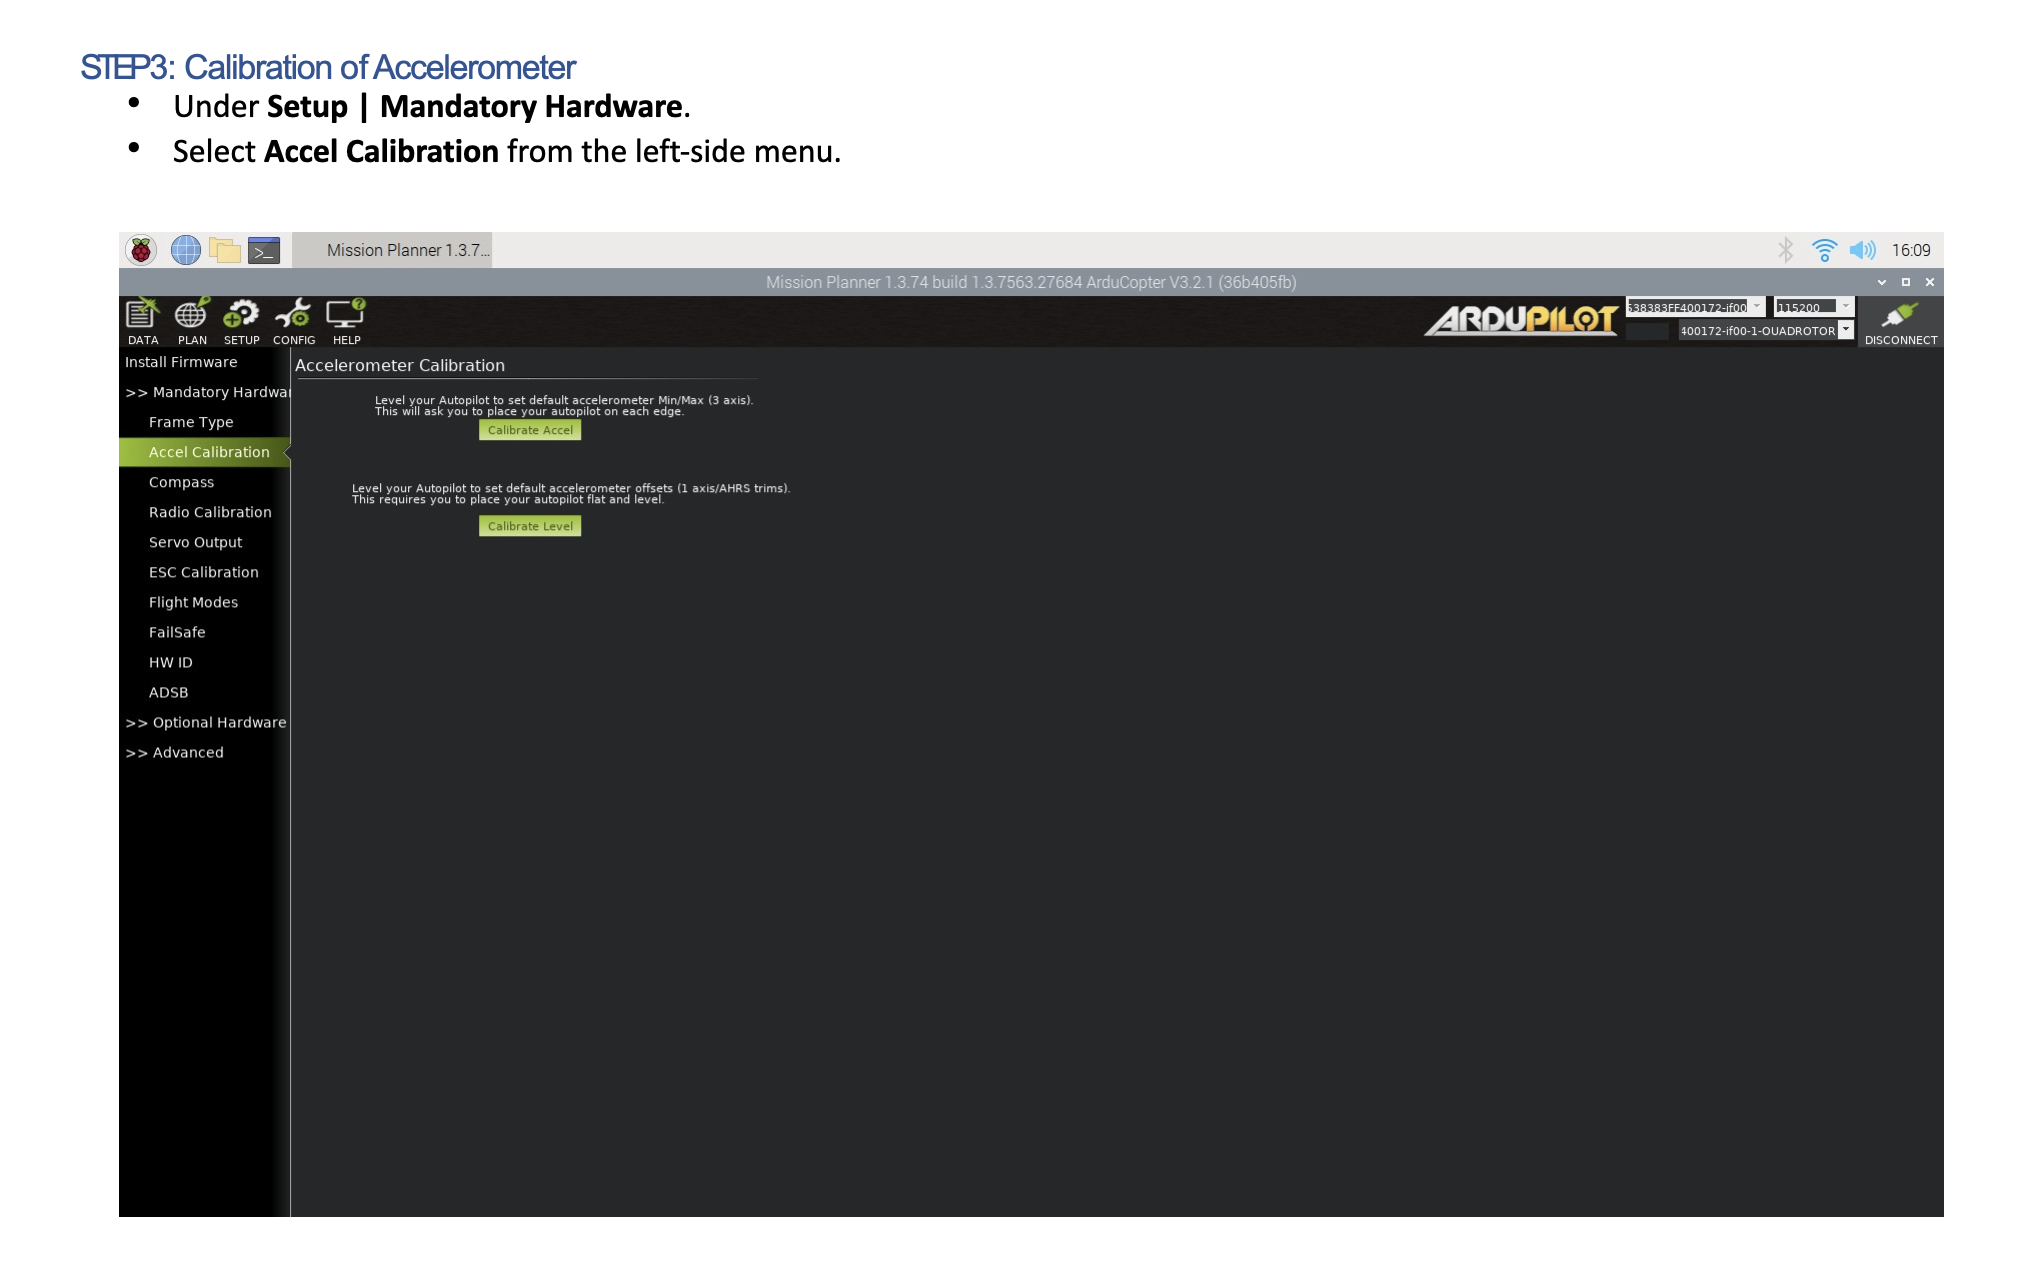
\includegraphics[width=\columnwidth]{./Figures/config_img26.png}
\end{figure}

\begin{figure}[h!]
\centering
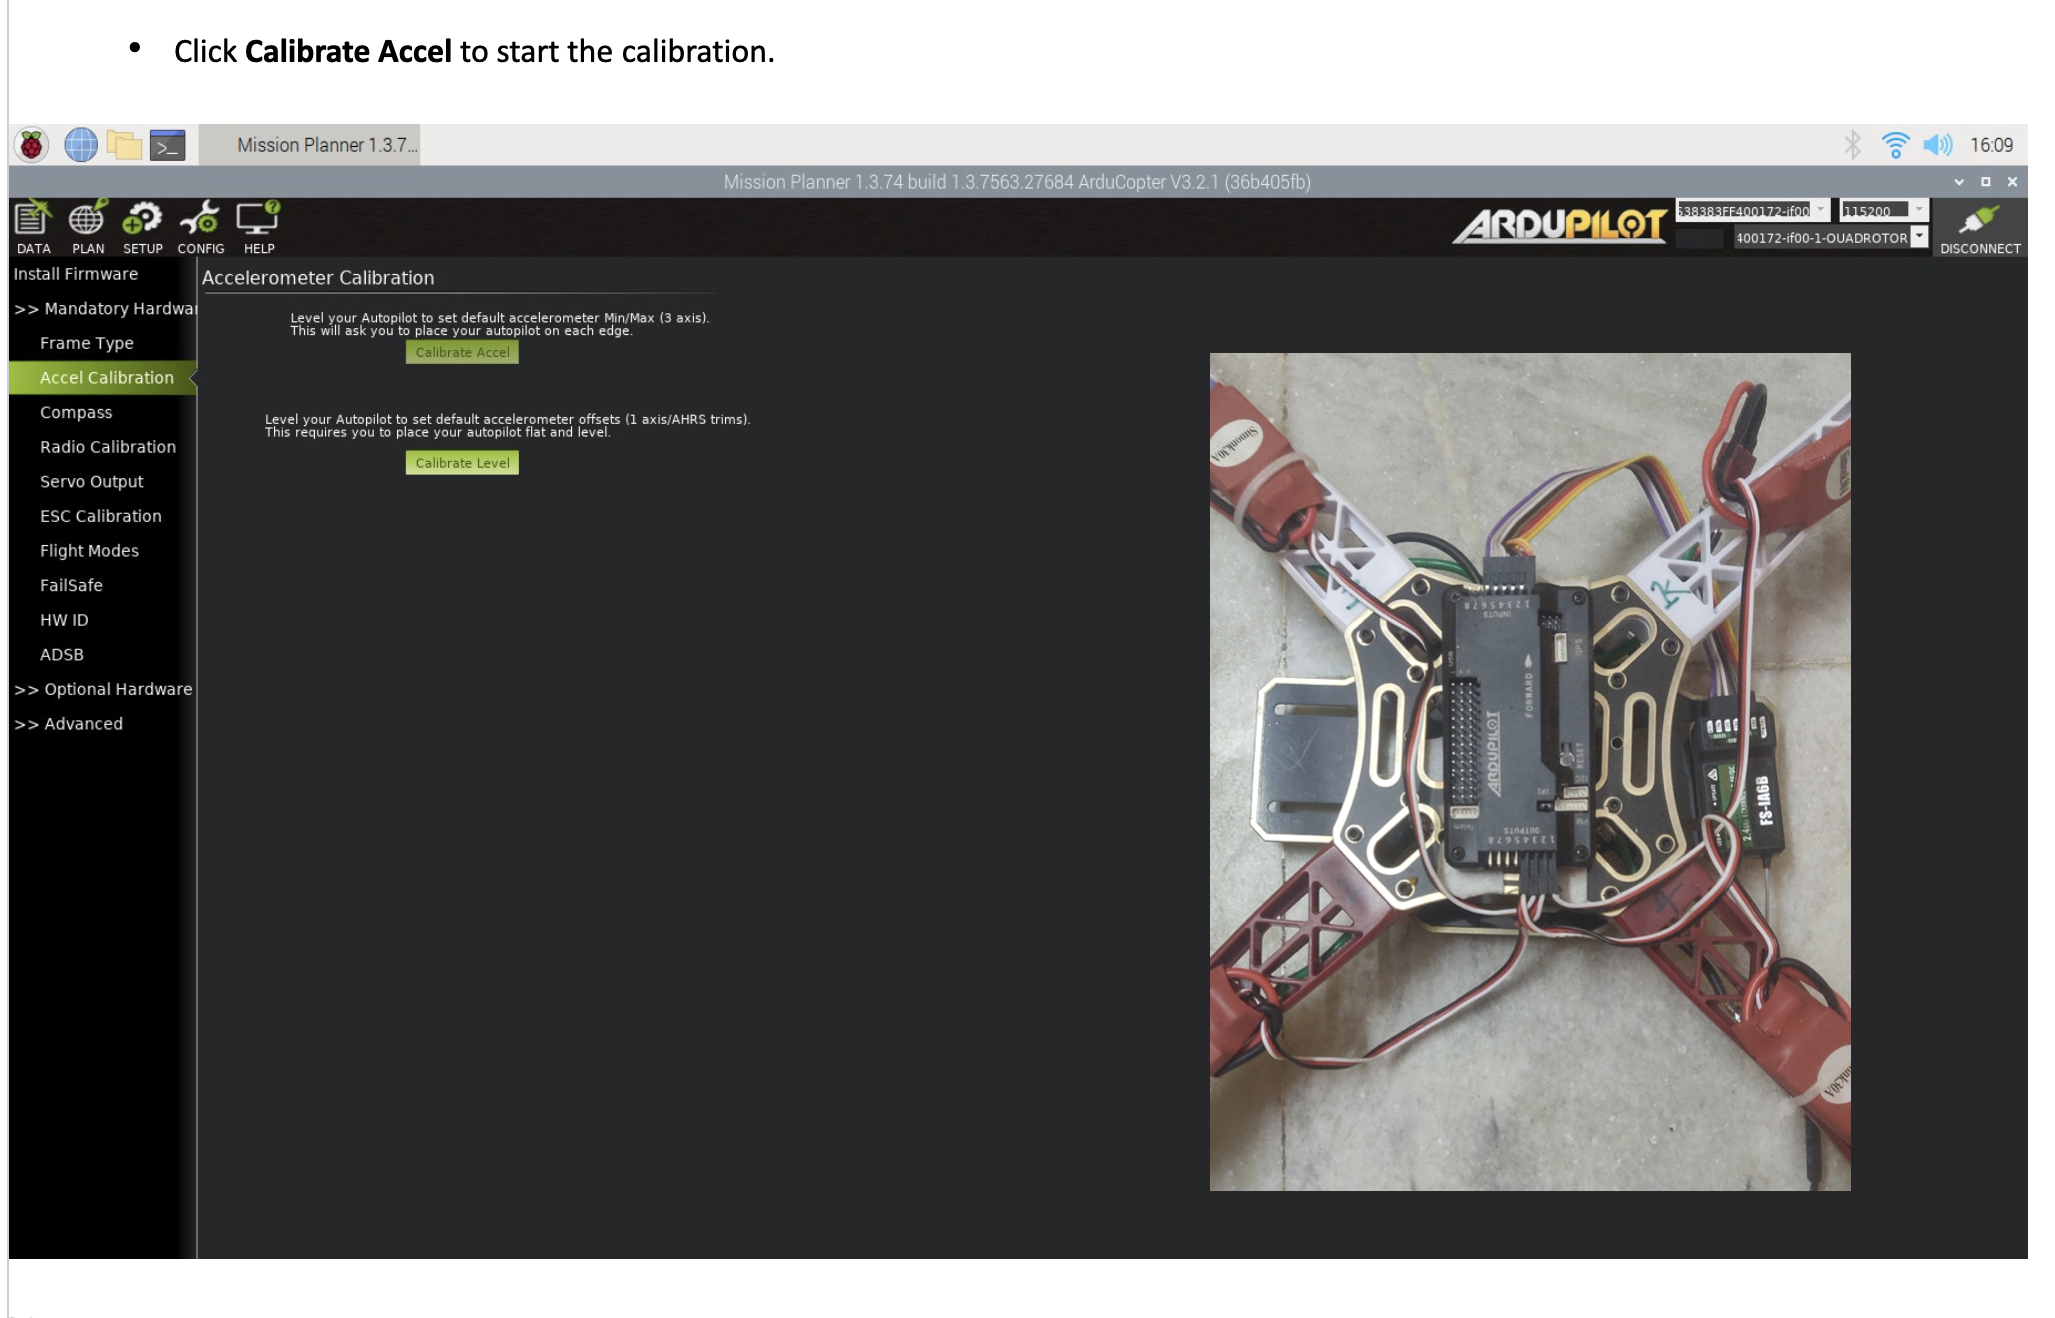
\includegraphics[width=\columnwidth]{./Figures/config_img27.png}
\end{figure}

\begin{figure}[h!]
\centering
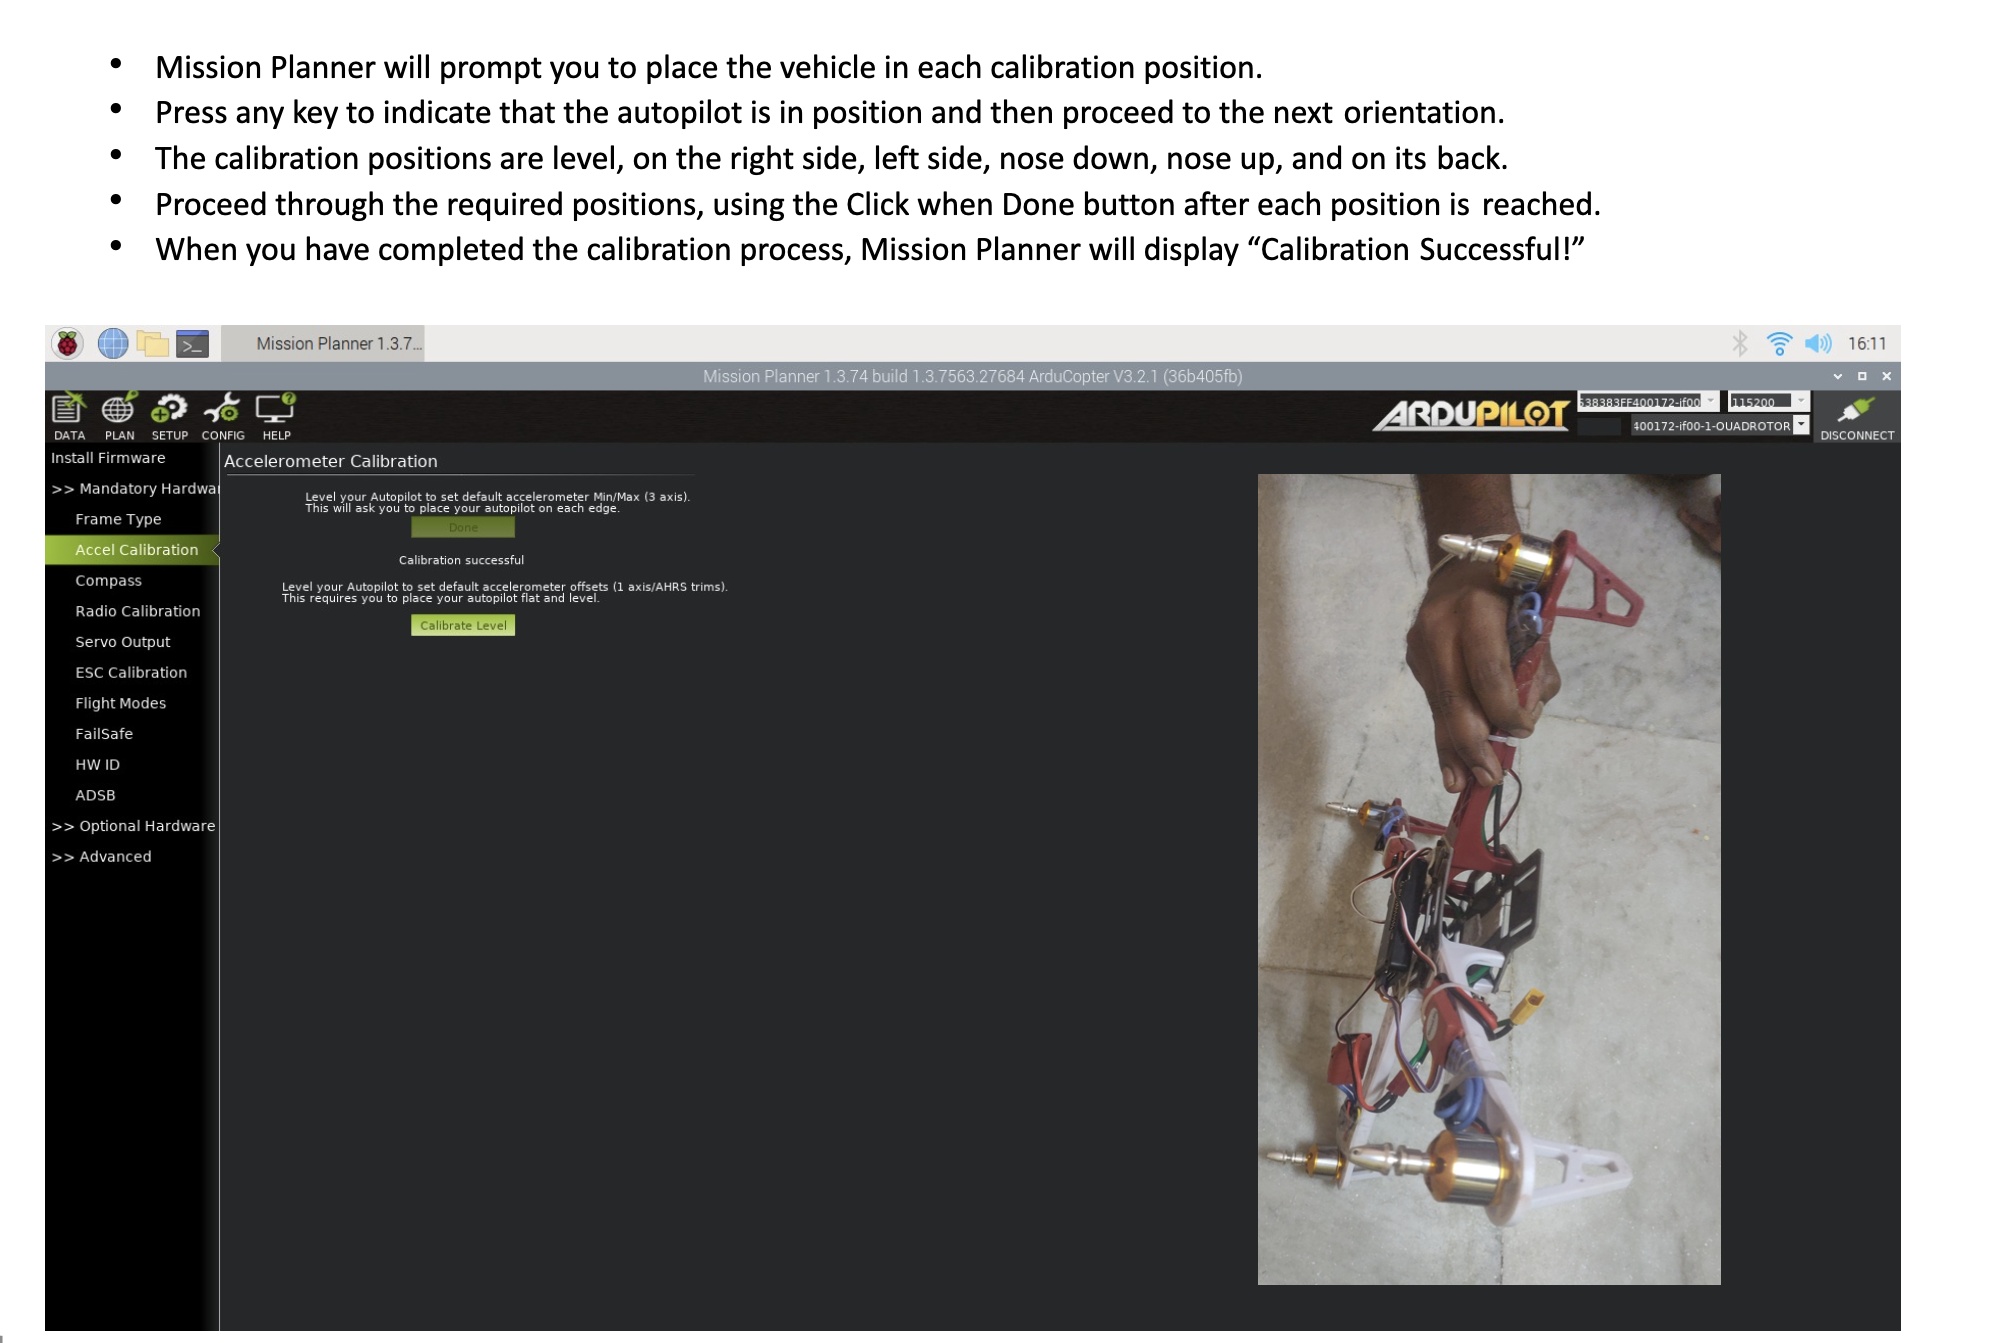
\includegraphics[width=\columnwidth]{./Figures/config_img28.png}
\end{figure}

\begin{figure}[h!]
\centering
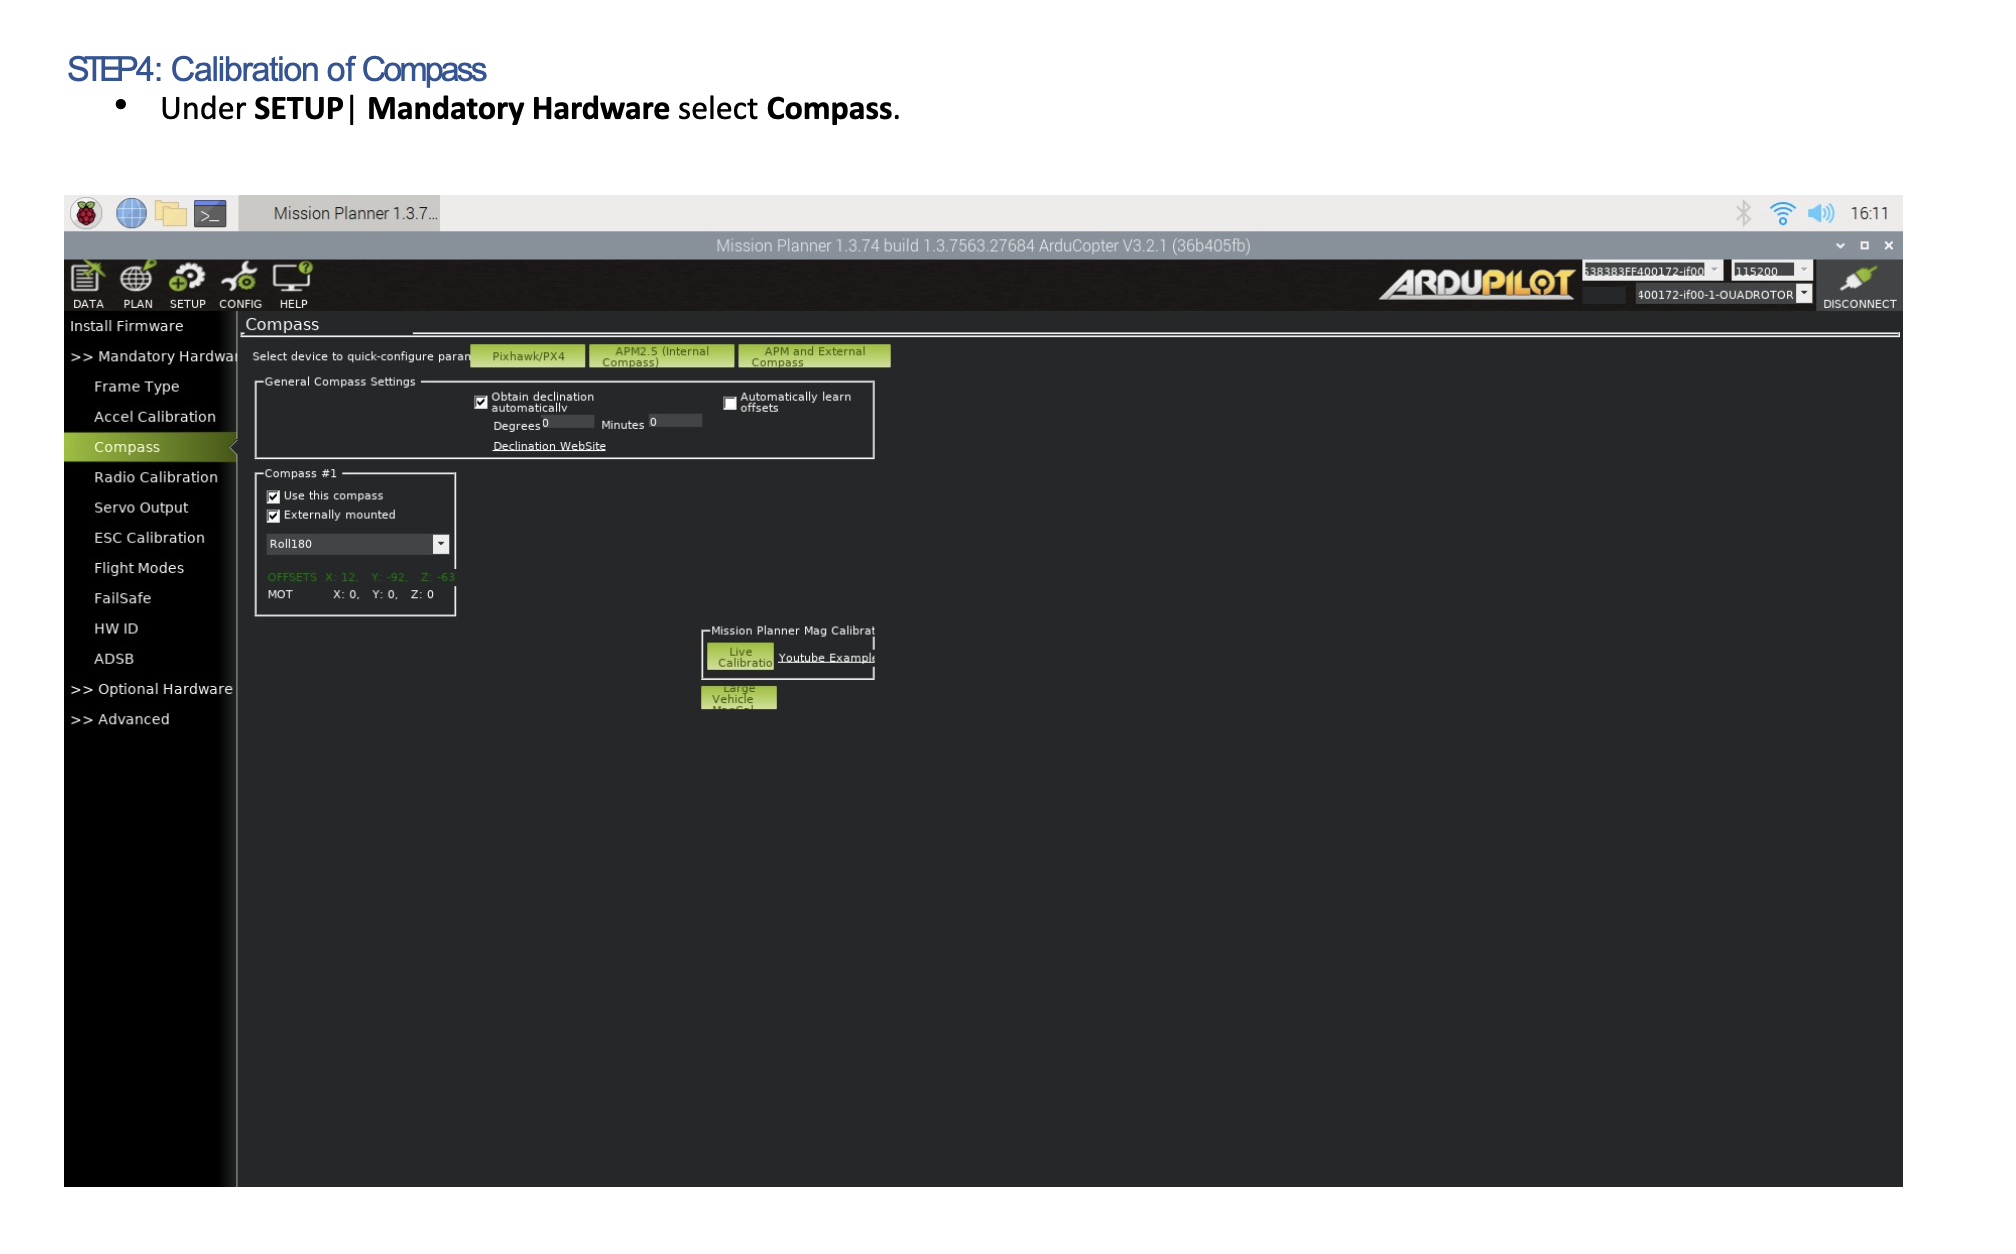
\includegraphics[width=\columnwidth]{./Figures/config_img29.png}
\end{figure}

\begin{figure}[h!]
\centering
\includegraphics[width=\columnwidth]{./Figures/config_img30.png}
\end{figure}

\begin{figure}[h!]
\centering
\includegraphics[width=\columnwidth]{./Figures/config_img31.png}
\end{figure}

\begin{figure}[h!]
\centering
\includegraphics[width=\columnwidth]{./Figures/config_img32.png}
\end{figure}

\begin{figure}[h!]
\centering
\includegraphics[width=\columnwidth]{./Figures/config_img33.png}
\end{figure}

\begin{figure}[h!]
\centering
\includegraphics[width=\columnwidth]{./Figures/config_img34.png}
\end{figure}

\begin{figure}[h!]
\centering
\includegraphics[width=\columnwidth]{./Figures/config_img35.png}
\end{figure}

\begin{figure}[h!]
\centering
\includegraphics[width=\columnwidth]{./Figures/config_img36.png}
\end{figure}

\begin{figure}[h!]
\centering
\includegraphics[width=\columnwidth]{./Figures/config_img37.png}
\end{figure}

\begin{figure}[h!]
\centering
\includegraphics[width=\columnwidth]{./Figures/config_img38.png}
\end{figure}

\begin{figure}[h!]
\centering
\includegraphics[width=\columnwidth]{./Figures/config_img39.png}
\end{figure}

\begin{figure}[h!]
\centering
\includegraphics[width=\columnwidth]{./Figures/config_img40.png}
\end{figure}



    
    